\documentclass[11pt,letterpaper]{article}

\addtolength{\oddsidemargin}{-.875in}
\addtolength{\evensidemargin}{-.875in}
\addtolength{\textwidth}{1.75in}

\addtolength{\topmargin}{-.875in}
\addtolength{\textheight}{1.75in}

\usepackage[utf8]{inputenc}
\usepackage{caption} % for table captions
\usepackage{amsmath} % for multi-line equations and piecewises
\DeclareMathOperator{\sign}{sign}
\usepackage{graphicx}
\usepackage{relsize}
\usepackage{xspace}
\usepackage{verbatim} % for block comments
% \usepackage{subcaption} % for subfigures
\usepackage{subfig}
\usepackage{enumitem} % for a) b) c) lists
\newcommand{\Cyclus}{\textsc{Cyclus}\xspace}%
\newcommand{\Cycamore}{\textsc{Cycamore}\xspace}%
\newcommand{\deploy}{\texttt{d3ploy}\xspace}%
\newcommand{\Deploy}{\texttt{D3ploy}\xspace}%
\usepackage{tabularx}
\usepackage{color}
\usepackage{multirow}
\usepackage{float}
\usepackage[acronym,toc]{glossaries}
\newacronym{ANL}{ANL}{Argonne National Laboratory}
\newacronym{B4C}{B4C}{boron carbide}
\newacronym{BC}{BC}{boundary condition}
\newacronym{BOC}{BOC}{beginning of equilibrium cycle}
\newacronym{BSD}{BSD}{Berkeley Software Distribution}
\newacronym{BWR}{BWR}{Boiling Water Reactor}
\newacronym{CAISO}{CAISO}{California ISO}
\newacronym{CEA}{CEA}{Commissariat a l'Energie Atomique}
\newacronym{CFD}{CFD}{computational fluid dynamics}
\newacronym{CO2}{CO$_2$}{carbon dioxide}
\newacronym{CR}{CR}{control rod}
\newacronym{CRP}{CRP}{Coordinated Research Project}
\newacronym{CZP}{CZP}{Cold Zero Power}
\newacronym{DCC}{DCC}{depressurized conduction cool-down}
\newacronym{DOE}{DOE}{Department of Energy}
\newacronym[\glslongpluralkey={degrees of freedom}]{DoF}{DoF}{degree of freedom}
\newacronym{EOC}{EOEC}{end of equilibrium cycle}
\newacronym{FCEV}{FCEV}{Fuel Cell Electric Vehicle}
\newacronym{FDM}{FDM}{Finite Difference Method}
\newacronym{FEM}{FEM}{Finite Element Method}
\newacronym{FVM}{FVM}{Finite Volume Method}
\newacronym{FSV}{FSV}{Fort St. Vrain}
\newacronym[\glslongpluralkey={greenhouse gases}]{GHG}{GHG}{greenhouse gas}
\newacronym{GRS}{GRS}{Gesellschaft für Anlagen und Reaktorsicherheit}
\newacronym{H2}{H$_2$}{hydrogen}
\newacronym{He}{He}{helium}
\newacronym{HFP}{HFP}{Hot Full Power}
\newacronym{HPCC}{HPCC}{high pressure conduction cool-down}
\newacronym{HTE}{HTE}{High-Temperature Electrolysis}
\newacronym{HTGR}{HTGR}{High-Temperature Gas-Cooled Reactor}
\newacronym{HTR}{HTR}{High Temperature Reactor}
\newacronym{HTTR}{HTTR}{High Temperature Test Reactor}
\newacronym{HZDR}{HZDR}{Helmholtz-Zentrum Dresden-Rossendorf}
\newacronym{IAEA}{IAEA}{International Atomic Energy Agency}
\newacronym{icap}{iCAP}{Illinois Climate Action Plan}
\newacronym{INL}{INL}{Idaho National Laboratory}
\newacronym{IPyC}{IPyC}{inner pyrolytic carbon}
\newacronym{JFNK}{JFNK}{Jacobian-Free Newton-Krylov}
\newacronym{KAERI}{KAERI}{Korea Atomic Energy Research Institute}
\newacronym{Keff}{K$_{eff}$}{multiplication factor}
\newacronym{LBP}{LBP}{Lumped Burnable Poison}
\newacronym{LGPL}{LGPL}{Lesser GNU Public License}
\newacronym{LOCA}{LOCA}{loss of coolant accident}
\newacronym{LPCC}{LPCC}{low pressure conduction cool-down}
\newacronym{LTE}{LTE}{Low-Temperature Electrolysis}
\newacronym{LWR}{LWR}{Light Water Reactor}
\newacronym{MC}{MC}{Monte Carlo}
\newacronym{MHTGR}{MHTGR}{Modular High-Temperature Gas-Cooled Reactor}
\newacronym{MOC}{MOC}{middle of equilibrium cycle}
\newacronym{MOOSE}{MOOSE}{Multi-physics Object-Oriented Simulation Environment}
\newacronym{MPI}{MPI}{Message Passing Interface}
\newacronym{MSR}{MSR}{Molten Salt Reactor}
\newacronym{MTD}{MTD}{Champaign-Urbana Mass Transit District}
\newacronym{NEA}{NEA}{Nuclear Energy Agency}
\newacronym{NEM}{NEM}{Nodal Expansion Method}
\newacronym{NGNP}{NGNP}{Next Generation Nuclear Power}
\newacronym{NRC}{NRC}{Nuclear Regulatory Commission}
\newacronym{NSC}{NSC}{Nuclear Science Committee}
\newacronym{OECD}{OECD}{Organisation for Economic Co-operation and Development}
\newacronym{OPyC}{OPyC}{outer pyrolytic carbon}
\newacronym{ORNL}{ORNL}{Oak Ridge National Laboratory}
\newacronym{OS}{OS}{Operator-Splitting}
\newacronym{PBMR}{PBMR}{Pebble Bed Modular Reactor}
\newacronym{PDE}{PDE}{Partial Differential Equation}
\newacronym{PMR}{PMR}{Prismatic Modular Reactor}
\newacronym{PV}{PV}{photovoltaics}
\newacronym{RSC}{RSC}{Reserve Shutdown Control}
\newacronym{RSD}{RSD}{Relative Standard Deviation}
\newacronym{SD}{SD}{Standard Deviation}
\newacronym{SI}{SI}{Sulfur-Iodine}
\newacronym{SiC}{SiC}{silicon carbide}
\newacronym{SMR}{SMR}{Small Modular Reactor}
\newacronym{SNU}{SNU}{Seoul National University}
\newacronym{SOEC}{SOEC}{Solid Oxide Electrolysis Cells}
\newacronym{TIP}{TIP}{transverse integration procedure}
\newacronym{TRISO}{TRISO}{Tristructural Isotropic}
\newacronym{UIUC}{UIUC}{University of Illinois at Urbana-Champaign}
\newacronym{UNIST}{UNIST}{Ulsan National Institute of Science and Technology}
\newacronym{UK}{UK}{United Kingdom}
\newacronym{UMICH}{UMICH}{University of Michigan}
\newacronym{US}{US}{United States}
\newacronym{VHTR}{VHTR}{Very High Temperature Gas Cooled Reactor}
%\newacronym{<++>}{<++>}{<++>}
%\newacronym{<++>}{<++>}{<++>}

\definecolor{bg}{rgb}{0.95,0.95,0.95}
\newcolumntype{b}{X}
\newcolumntype{f}{>{\hsize=.15\hsize}X}
\newcolumntype{s}{>{\hsize=.5\hsize}X}
\newcolumntype{m}{>{\hsize=.75\hsize}X}
\newcolumntype{r}{>{\hsize=1.1\hsize}X}
\usepackage{titling}
\usepackage[hang,flushmargin]{footmisc}
\renewcommand*\footnoterule{}
\usepackage{tikz}
\usepackage{array}
\usepackage{booktabs,mathptmx,siunitx}
\sisetup{input-symbols = {()},  % do not treat "(" and ")" in any special way
         group-digits  = false} % no grouping of digits

\usetikzlibrary{shapes.geometric,arrows}
\tikzstyle{process} = [rectangle, rounded corners,
minimum width=1cm, minimum height=1cm,text centered, draw=black,
fill=blue!30]
\tikzstyle{arrow} = [thick,->,>=stealth]

\graphicspath{}

\begin{document}

\section{Preliminary studies}

\subsection{Homogeneous vs heterogeneous isotope distribution}

This study modeled two different isotope distributions in a fuel compact.
First, a homogeneous distribution of the isotopes.
Second, a heterogeneous distribution, in which we explicitly model the TRISO particles.
We modeled both cases using Serpent.
We used a hexagonal unit cell model that includes the fuel compact, a helium gap, and the surrounding graphite.
Table \ref{tab:compact} specifies the model input parameters.
The material temperature was 1200K, case that represents the \gls{HFP} core state.
Serpent ran 5$\times 10^4$ neutrons/cycle, 500 active cycles, and 50 inactive cycles for the calculations.
The simulations took 1.73 and 2.21 minutes using 256 cores.
The heterogeneous calculations took a 28$\%$ more.

The \gls{Keff} was 1.17523 for the homogeneous case and 1.25106 for the heterogeneous case.
Using the heterogeneous case as the reference result, we calculated the relative error of the most relevant group constants in an eigenvalue calculation.
Serpent generated the group constants using the three energy group structure in Table \ref{tab:energygroups}.
The evaluated parameters were $D_g$, $\Sigma^r_g$, $\nu\Sigma^f_g$, and $\chi^t_g$ (see equation \ref{eq:diffusion}).
Figure \ref{fig:param-comparison} displays the relative errors for $\Sigma^r_g$ and $\nu\Sigma^f_g$, which were the group constants that changed the most.
The figure does not include relative errors for $D_g$ and $\chi^t_g$ because they were less than 1$\%$.
The relative errors of $\Sigma^r_g$ and $\nu\Sigma^f_g$ were less than 6$\%$.

% \cite{strydom_results_2015}
% The low multiplication factor in the homogeneous case is due to the fuel self-shielding .
% In the heterogeneous compact, the fuel self-shielding leads to a significantly decreased U-238 neutron absorption compared to the homogeneous fuel compact.

\begin{figure}[htbp!]
	\centering
	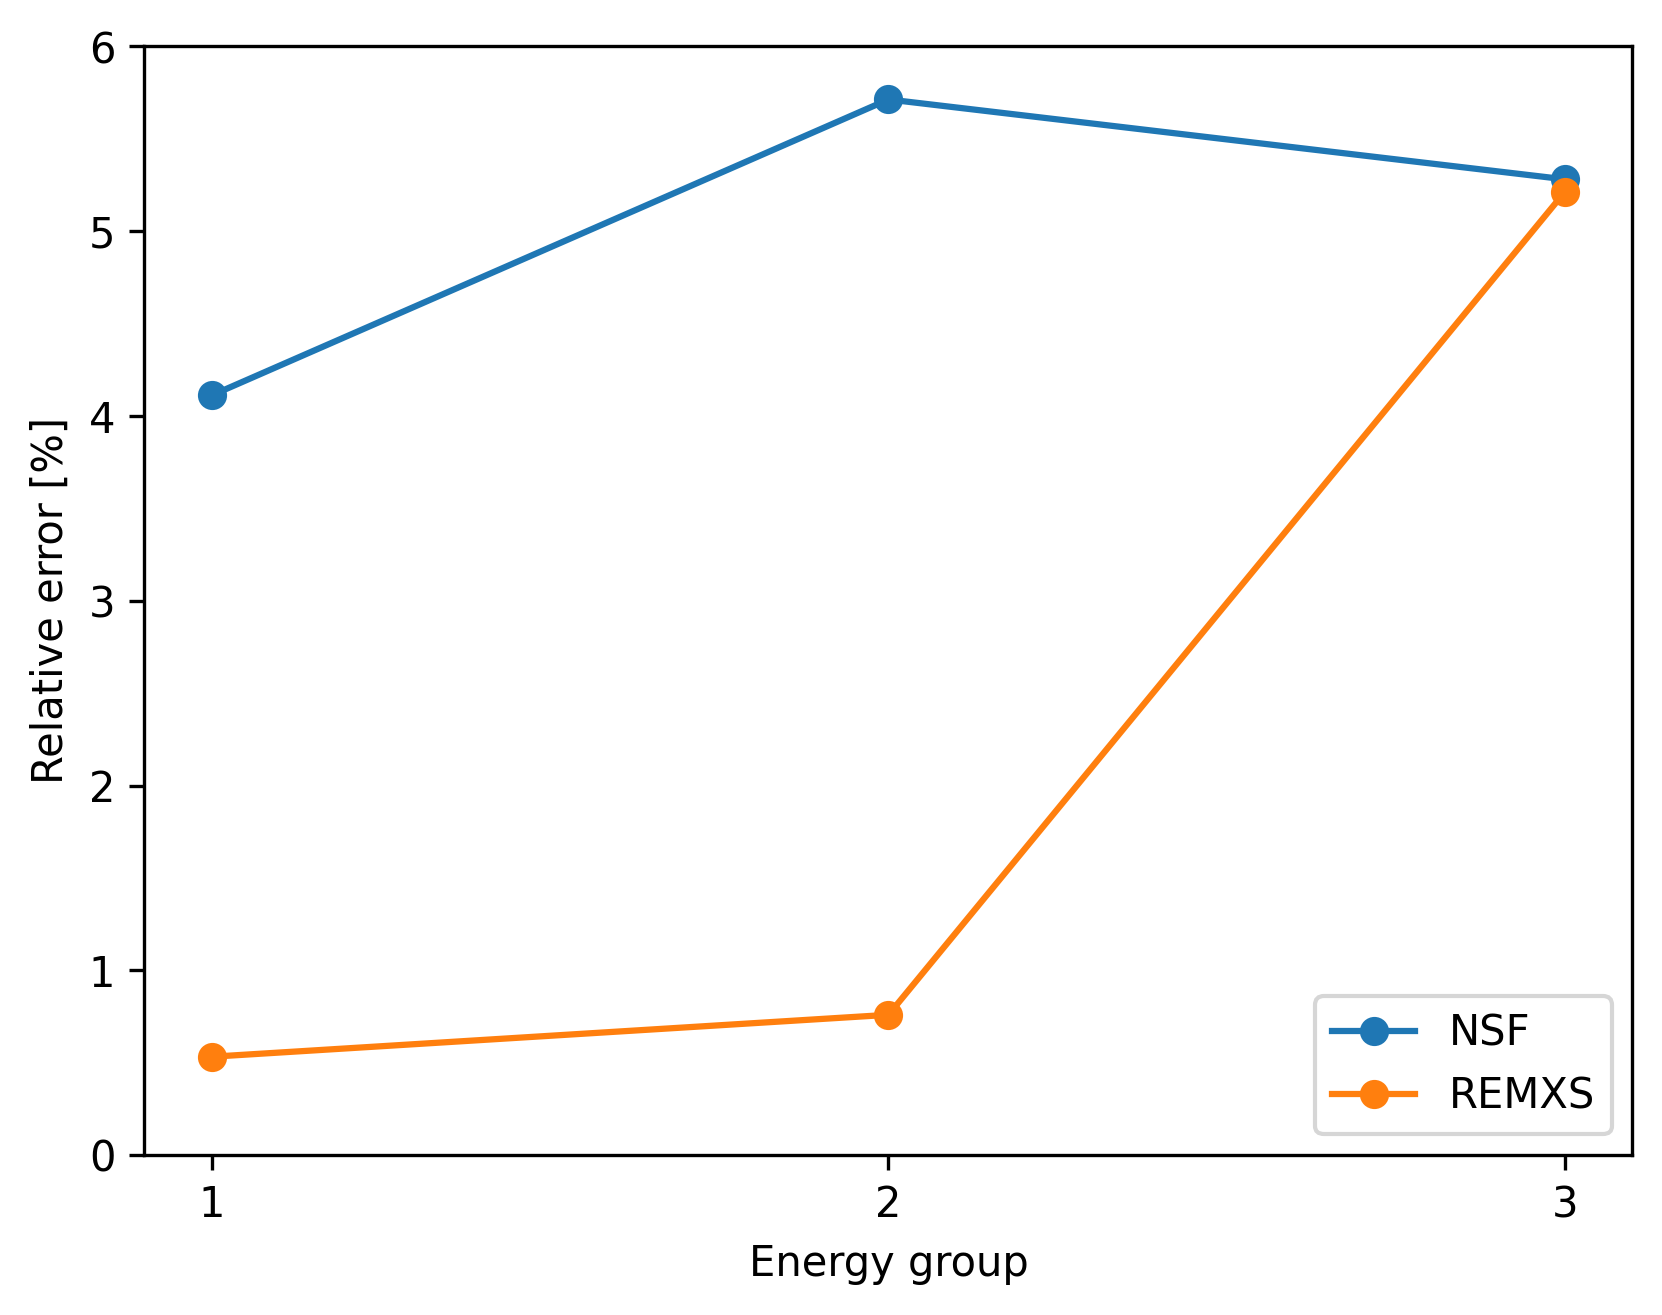
\includegraphics[width=0.45\linewidth]{figures/param-comparison}
	\hfill
	\caption{Relative error of the group constants generated with a homogeneous isotope distribution.}
	\label{fig:param-comparison}
\end{figure}

\subsection{Moltres limitations}

Serpent run 5$\times 10^5$ neutrons/cycle, 400 active cycles, and 100 inactive cycles for the calculations.
The \gls{Keff} was 1.41933.

Moltres
Mesh: dof/group ()
Keff = 

Figures

% Maybe here or next section
Based on these results and discussions, in the following sections, we obtain the homogenized group constants.
In the fuel block, the fuel, coolant, and moderator all share the same group constants.

\section{Serpent-Moltres comparison}

\subsection{Fuel column}

In this section, we investigated the effects of the choice of energy group structure on the diffusion simulations.
We conducted two analyses.
First, we varied the number of energy groups.
Second, we tried different energy group structures for the same number of groups.
To reduce the computational expense we narrowed down our focus to a fuel column of the MHTGR-350, Figure \ref{fig:fuelcolumn}.
The fuel column includes the bottom and top reflectors.
Tables \ref{tab:element-characteristics} and \ref{tab:compact} specify the model input parameters.

The first step in the calculation was to obtain the group constants using Serpent.
Figure \ref{fig:fuelcolumn} displays the $xy$-plane of the model.
To simplify Serpent's model, we did not consider the fuel handling holes nor the coolant channels in the bottom and top reflectors.
\glspl{HTGR} use \glspl{LBP} to reduce the peaking factors in different regions of the active core.
Some reactors could have \glspl{LBP} in the rings closer to the reflectors, and no \glspl{LBP} in the middle rings.
This motivated the analysis of two cases, a fuel column that does not have \glspl{LBP}, and one that has.
The LBP's locations are the six corners of the fuel assembly, Figure \ref{fig:fuelcolumn}.
The material temperatures were 600K and 1200K, cases that represent the \gls{CZP} and the \gls{HFP} core states.
Serpent ran 4$\times 10^5$ neutrons/cycle, 360 active cycles, and 40 inactive cycles for the calculations.

We made the geometry and mesh using Gmsh \cite{geuzaine_gmsh_2020}.
Taking advantage of the symmetry of the problem, the model included only a one-twelfth of the fuel column.
The mesh had 37120 elements and 22862 nodes.
The diffusion calculations had 22862 \glspl{DoF}/energy-group.
The Moltres input files set an eigenvalue and a flux convergence tolerance of 1$\times$10$^{-8}$.
The calculations in Moltres used different energy group structures listed in Table \ref{tab:energygroups}.

% This is very important and I should review it carefully
To compare the results from Serpent and Moltres, we present a figure comparing the three-group axial flux.
Moltres ran the calculations for 26 energy groups, and collapsed the results to three energy groups to facilitate the visualization of the results.
Note that the flux in Serpent is an average over the volume, while the flux in Moltres is the point-wise flux over a line.
Another figure compares the eigenvalue from Serpent and eigenvalues from Moltres for the different energy group structures.
The last analysis is for the Moltres axial flux.
Considering the 26 group structure as the reference value, we obtained the L2-norm relative error for the axial flux in the active core.

% Fluxes
To recapitulate, we simulated four operational cases: no \gls{LBP} at 600K, no \gls{LBP} at 1200K, \gls{LBP} at 600K, and \gls{LBP} at 1200K.
Figures \ref{fig:assembly-noLBP-600-flux} to \ref{fig:assembly-LBP-1200-flux} display the axial flux from the Serpent and the Moltres simulations for all cases.
For the no LBP at 600K case, the fluxes are close in shape and magnitude.
For the no LBP at 1200K case, the fluxes look similar.
The flux in Moltres has a more straight shape.
The thermal flux peak in the bottom reflector has a bigger magnitude.
For the LBP at 600K case, the flux in Moltres has a bigger magnitude.
Additionally, the shape of the Moltres flux is concave while the Serpent flux is convex.
For the LBP at 1200K case, the flux in Moltres is bigger.
The Moltres flux is more concave than the Serpent flux.
Overall, the fluxes in Moltres and Serpent are close.

% eigenvalues
Table \ref{tab:keff} exhibits the reactivity difference ($\Delta \rho$) between the Serpent and Moltres eigenvalues.
We used equation \ref{eq:delta-rho} to obtain $\Delta \rho$.
The eigenvalues in Moltres differ slightly from the eigenvalues in Serpent.
Overall, the reactivity difference is less than 50 pcm.
We note that the number of energy groups does not affect the accuracy of the eigenvalue calculations in Moltres.

\begin{align}
	\Delta \rho &= \left| \frac{k_1-k_2}{k_1 k_2} \right| \label{eq:delta-rho}
  \intertext{where}
  k_1 &= \mbox{Serpent eigenvalue} \notag \\
  k_2 &= \mbox{Moltres eigenvalue.} \notag
\end{align}

Figures \ref{fig:assembly-noLBP-er} and \ref{fig:assembly-LBP-er} show the $L_2$-norm relative error for the different energy group structures.
We note that the relative error for the no LBP case is smaller than the relative error of the LBP case.
Overall, the relative error decreases with an increase in the number of energy groups.
Nonetheless, this is not always the case.
For example, in Figure \ref{fig:assembly-noLBP-er-b}, going from 12 to 15 groups, the thermal flux improves, but the fast flux worsens.
Additionally, we observe that a low number of energy groups yields an error of more than a 100$\%$.
In which, case we can conclude that the solution is wrong.

We added to the analysis the computational time and the peak memory usage during the simulations, Figure \ref{fig:assembly-time}.
All the simulations used 128 cores.
We present only the cases at 600K because the change in temperature does not have a significant impact.
The computational requirements rises with an increase in the number of energy groups.
As the geometry uses a constant number of elements, the DoFs/energy-group is constant.
Thus, the total number of DoFs is proportional to the number of energy groups.
We also discern that the overall time of the LBP cases is higher than the no LBP cases.

Finally, we analyzed the impact of changing the energy group structure for a constant number of energy groups.
We chose 15 energy groups, as it gives an overall good accuracy and a not so high computational expense.

Table \ref{tab:energygroups} holds the different energy group structures.
Table \ref{tab:accuracy15} exhibits the $L_2$-norm relative error for the different energy group structures.
We see that the energy group structure has an impact over the accuracy.
Some energy groups structures yield better results for some cases while giving worse results for others.
For example, the structure $15d$ gives better results for the LBP at 600K case than for the no LBP case at 600K.
In order to choose the best performing structure, we used a weighted average for the different groups.
We arbitrarily chose the weights to be 0.5, 0.3, and 0.2 for the thermal, epithermal, and fast fluxes.
Using this averaging scheme, we determined the group structure $15d$ to be the best one.

\begin{figure}[htbp!]
	\centering
    \subfloat[Fuel column geometry. Image reproduced form \cite{tak_numerical_2008}.]{
        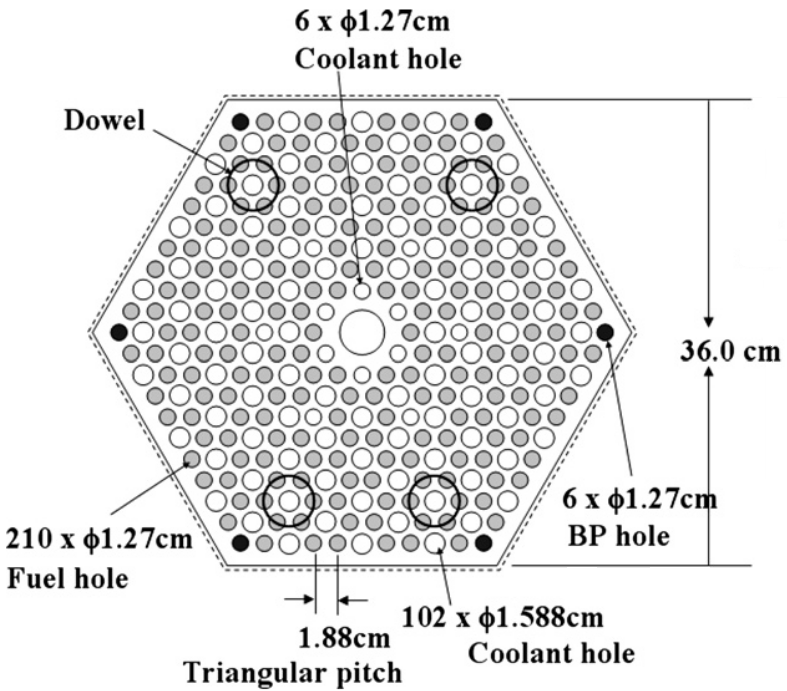
\includegraphics[width=0.51\textwidth]{figures-assembly/fuel-assembly}
    }
    \subfloat[Serpent model geometry.]{
        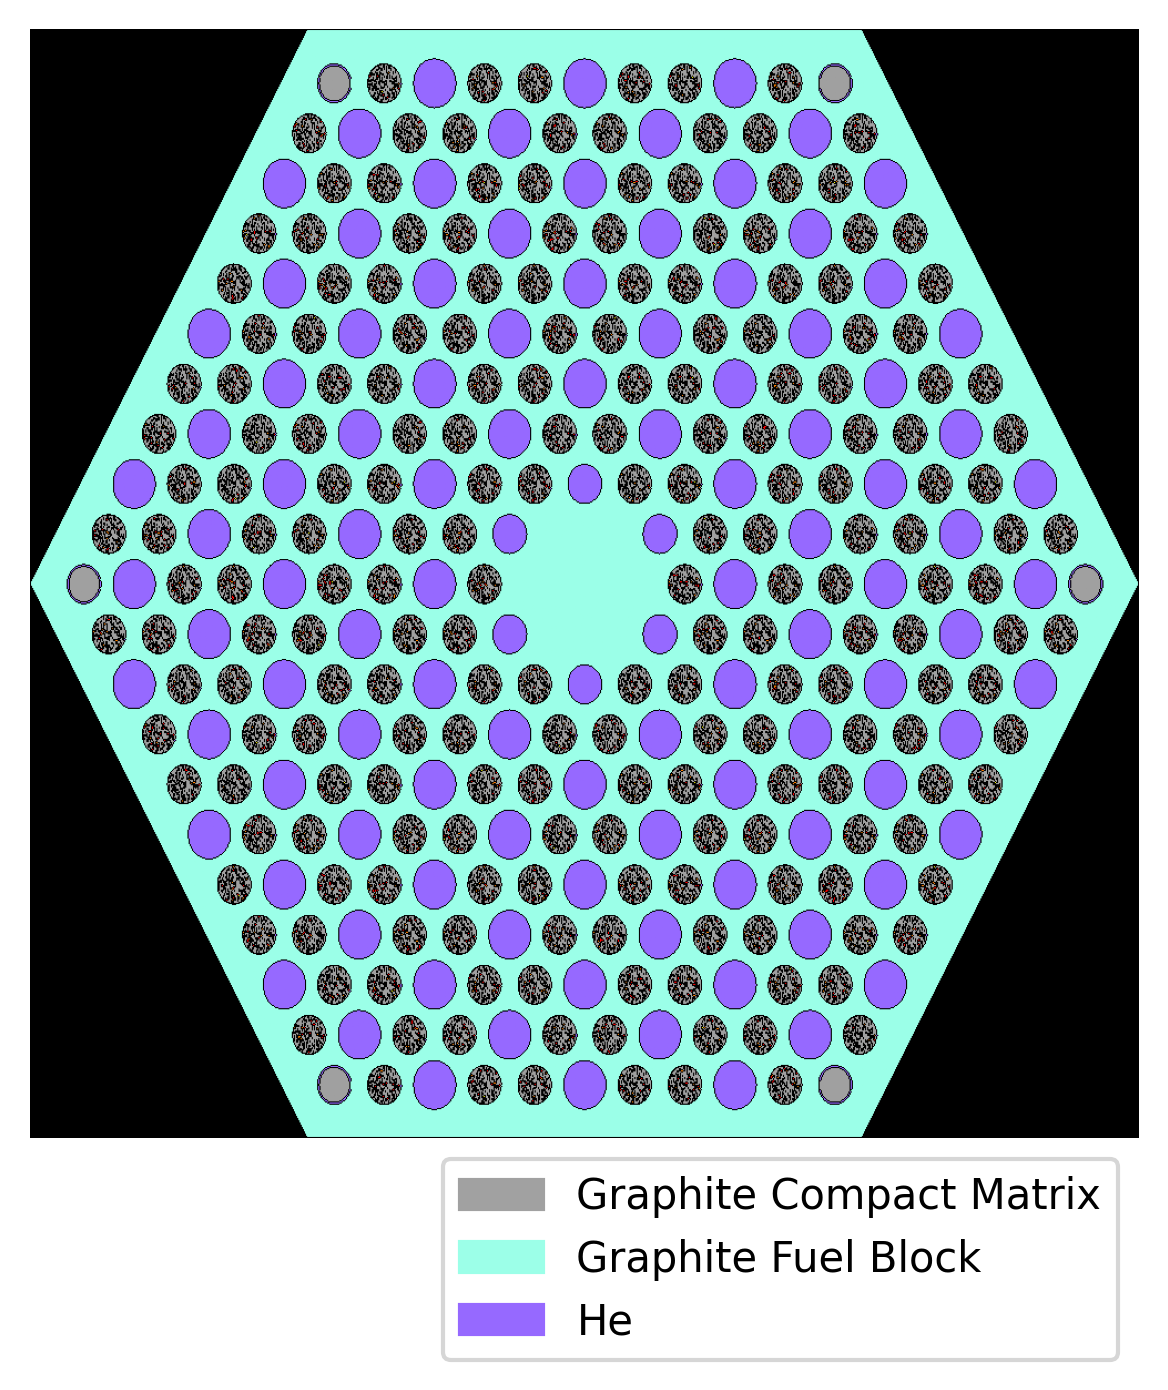
\includegraphics[width=0.34\textwidth]{figures-assembly/oecd-standard-column-legend}
    }
	\hfill
    \caption{Fuel column of the MHTGR-350. XY-plane in the active core region.}
	\label{fig:fuelcolumn}
\end{figure}

\begin{table}[htbp!]
  \centering
  \caption{Energy group structure.}
  \begin{tabular}{c|l|l|l|l|l|l|l|l|l|l|l|l}
  \toprule
  Upper boundary [eV] & 26    & 21   & 18   & 15a & 15b & 15c & 15d & 15e   & 12  & 9  & 6  & 3 \\
  \midrule
  1.49E+07            & 1     & 1    & 1    & 1   & 1   & 1   & 1   & 1     & 1   & 1  & 1  & 1 \\ \cline{1-2}
  7.41E+06            & 2     &      &      &     &     &     &     &       &     &    &    &   \\ \cline{1-10}
  3.68E+06            & 3     & 2    & 2    & 2   & 2   & 2   & 2   & 2     & 2   &    &    &   \\ \cline{1-2}
  6.72E+05            & 4     &      &      &     &     &     &     &       &     &    &    &   \\ \hline
  1.11E+05            & 5     & 3    & 3    & 3   & 3   & 3   & 3   & 3     & 3   & 2  & 2  & 2 \\ \cline{1-6} \cline{10-10}
  1.93E+04            & 6     & 4    & 4    & 4   & 4   &     &     &       & 4   &    &    &   \\ \cline{1-2}
  3.35E+03            & 7     &      &      &     &     &     &     &       &     &    &    &   \\ \cline{1-4} \cline{7-7}
  1.58E+03            & 8     & 5    & 5    &     &     & 4   &     &       &     &    &    &   \\ \cline{1-6} \cline{8-11}
  7.48E+02            & 9     & 6    & 6    & 5   & 5   &     & 4   & 4     & 5   & 3  &    &   \\ \cline{1-7} \cline{10-11}
  2.75E+02            & 10    & 7    & 7    & 6   & 6   & 5   &     &       & 6   & 4  &    &   \\ \cline{1-6} \cline{8-12}
  1.30E+02            & 11    & 8    & 8    & 7   & 7   &     & 5   & 5     & 7   & 5  & 3  &   \\ \cline{1-3} \cline{6-7}
  6.14E+01            & 12    & 9    &      &     & 8   & 6   &     &       &     &    &    &   \\ \cline{1-6} \cline{8-9}
  2.90E+01            & 13    & 10   & 9    & 8   & 9   &     & 6   & 6     &     &    &    &   \\ \cline{1-5} \cline{10-11}
  1.37E+01            & 14    & 11   & 10   & 9   &     &     &     &       & 8   & 6  &    &   \\ \cline{1-10}
  8.32E+00            & 15    & 12   & 11   & 10  & 10  & 7   & 7   & 7     & 9   &    &    &   \\ \cline{1-2}
  5.04E+00            & 16    &      &      &     &     &     &     &       &     &    &    &   \\ \hline
  2.38E+00            & 17    & 13   & 12   & 11  & 11  & 8   & 8   & 8     & 10  & 7  & 4  & 3 \\ \cline{1-3}
  1.29E+00            & 18    & 14   &      &     &     &     &     &       &     &    &    &   \\ \cline{1-12} 
  6.50E-01            & 19    & 15   & 13   & 12  & 12  & 9   & 9   & 9     & 11  & 8  & 5  &   \\ \cline{1-3} \cline{7-8}
  3.50E-01            & 20    & 16   &      &     &     & 10  & 10  &       &     &    &    &   \\ \cline{1-9}
  2.00E-01            & 21    & 17   & 14   & 13  & 13  & 11  & 11  & 10    &     &    &    &   \\ \cline{1-2} \cline{9-9}
  1.20E-01            & 22    &      &      &     &     &     &     & 11    &     &    &    &   \\ \cline{1-9} 
  8.00E-02            & 23    & 18   & 15   & 14  & 14  & 12  & 12  & 12    &     &    &    &   \\ \cline{1-4} \cline{7-9}
  5.00E-02            & 24    & 19   & 16   &     &     & 13  & 13  & 13    &     &    &    &   \\ \hline
  2.00E-02            & 25    & 20   & 17   & 15  & 15  & 14  & 14  & 14    & 12  & 9  & 6  &   \\ \cline{1-4} \cline{7-9}
  1.00E-02            & 26    & 21   & 18   &     &     & 15  & 15  & 15    &     &    &    &   \\
  \bottomrule
  \end{tabular}
  \label{tab:energygroups}
\end{table}

% No LBP 600
\begin{figure}[htbp!]
	\centering
    \subfloat[Moltres.]{
        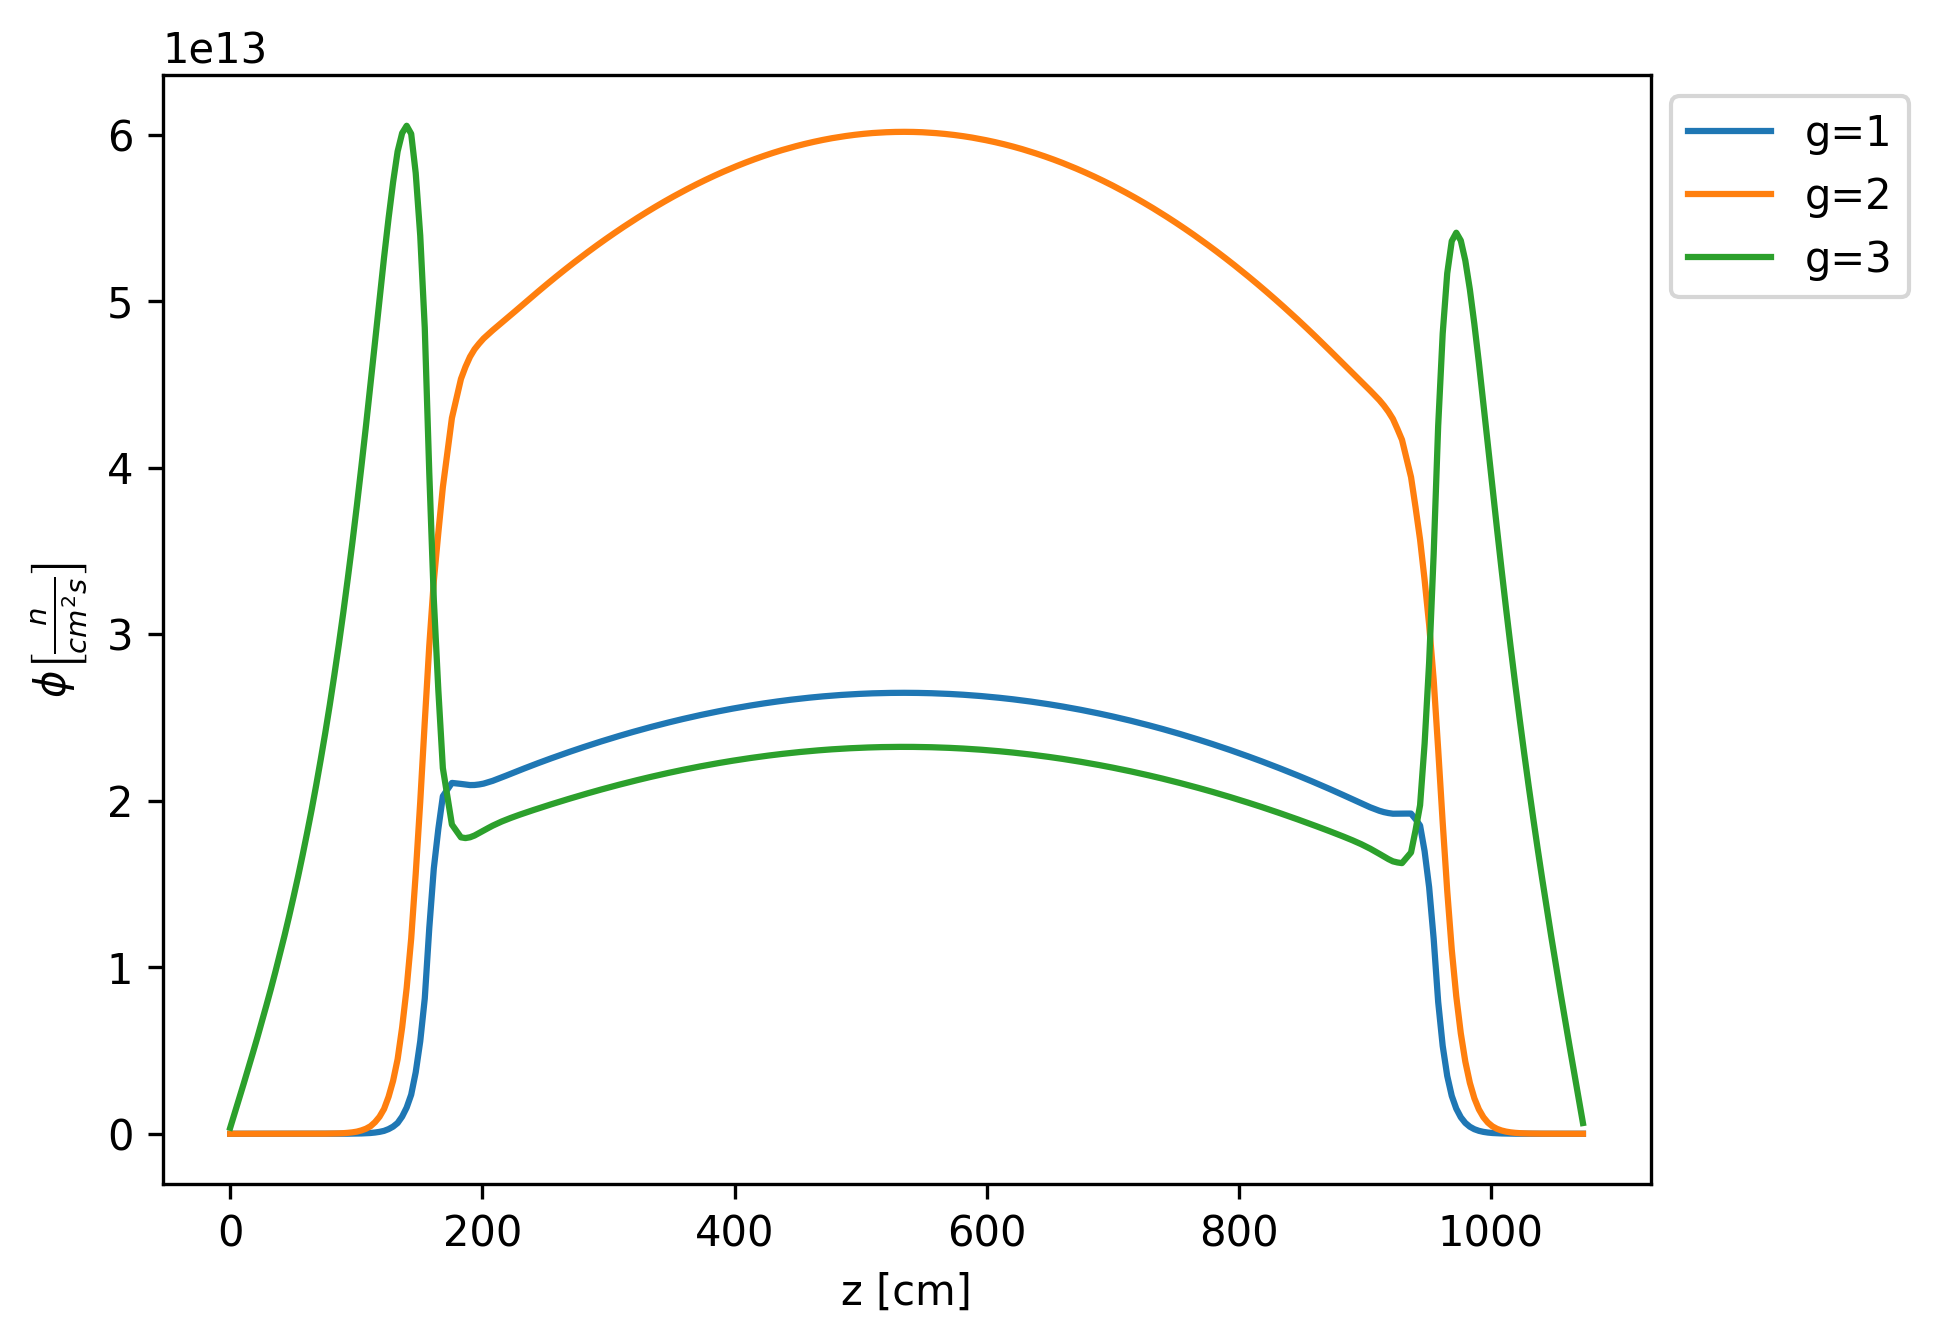
\includegraphics[width=0.45\textwidth]{figures-assembly/3D-assembly-noLBP-600-26G}
    }
    \subfloat[Serpent.]{
        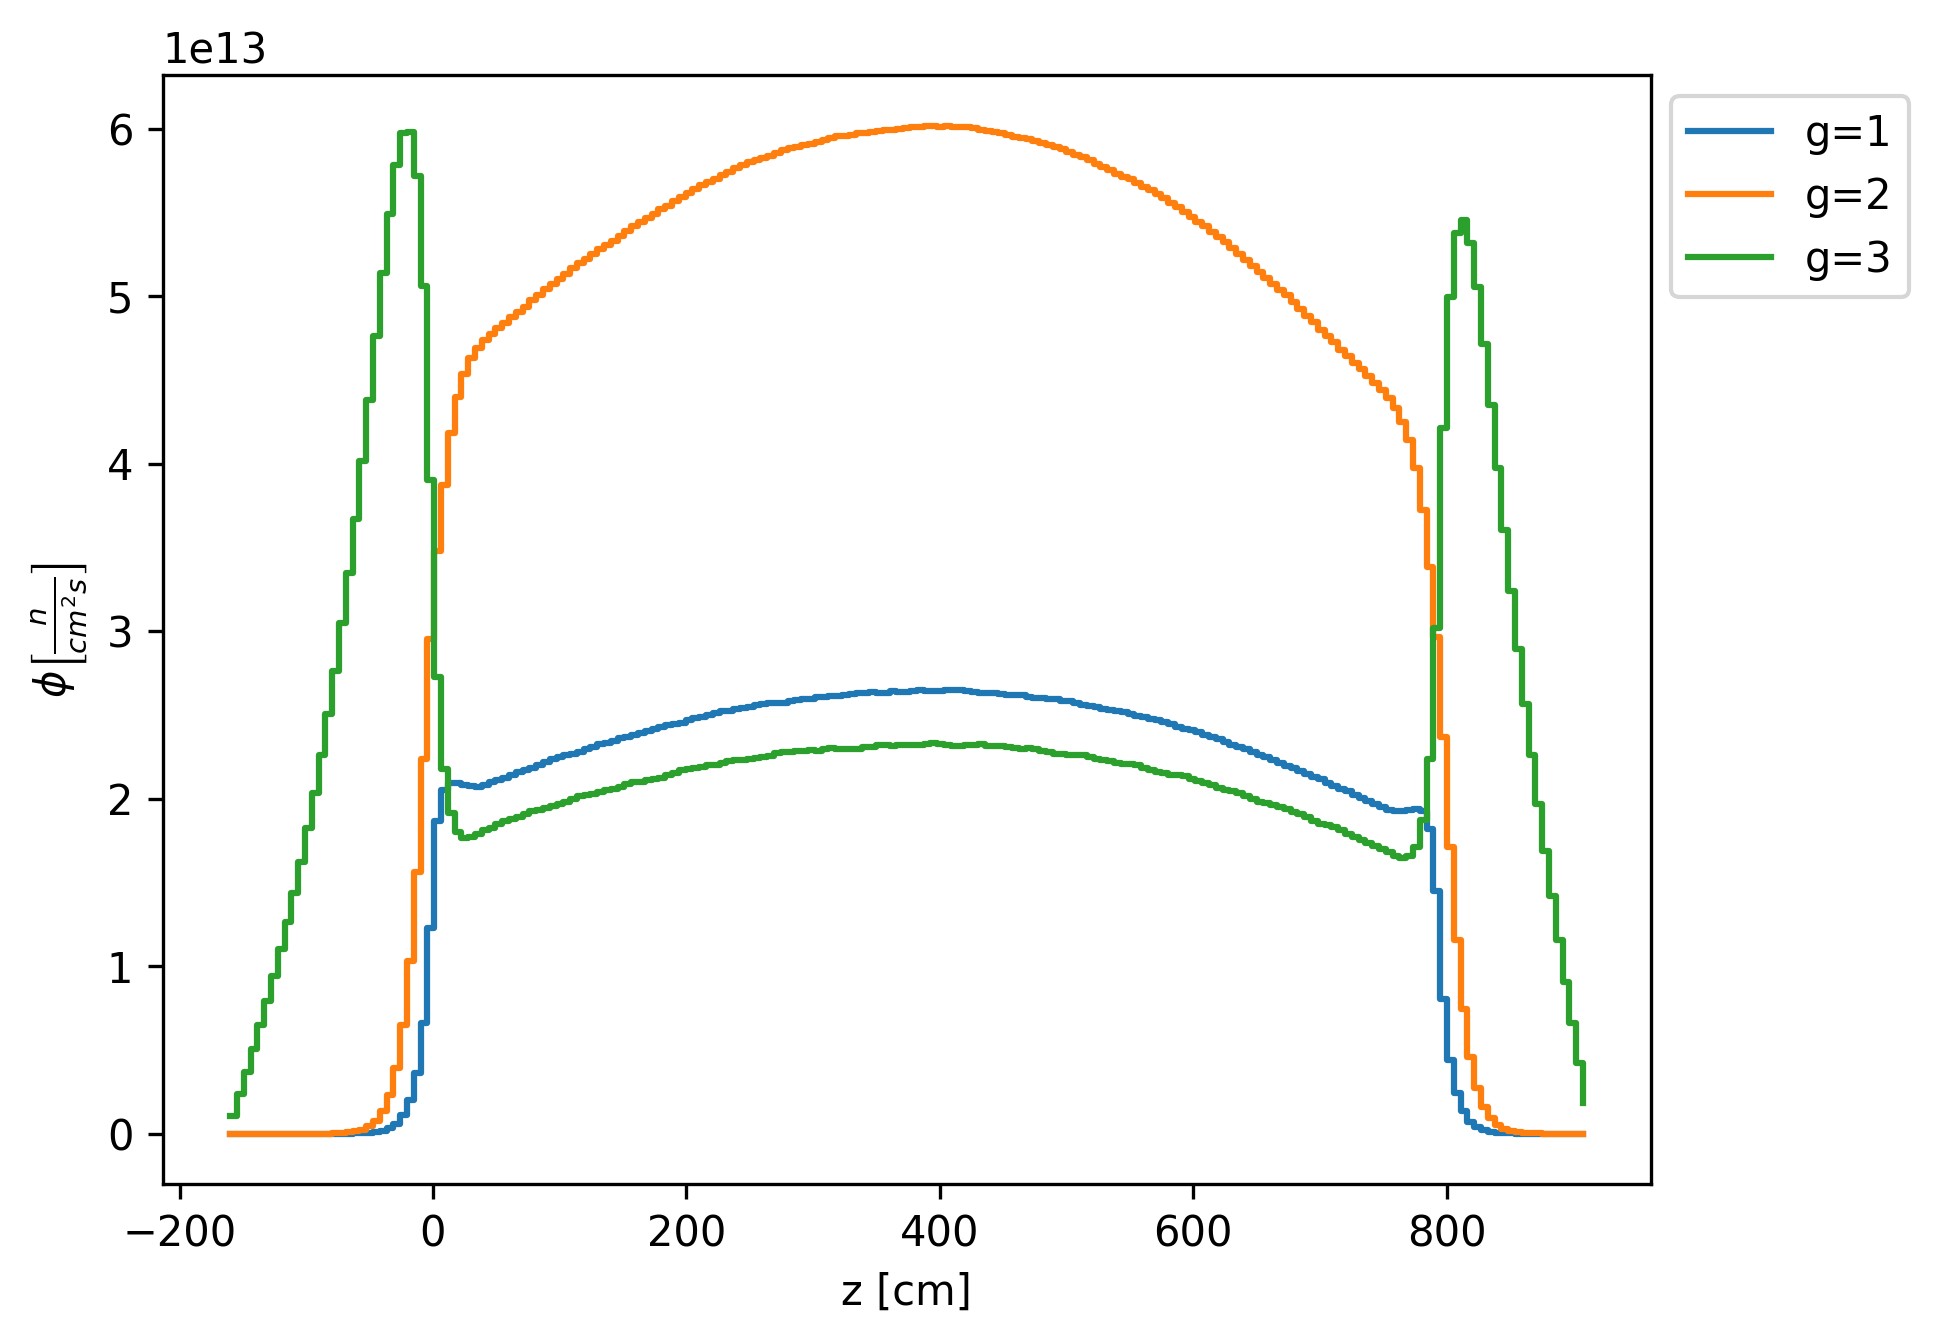
\includegraphics[width=0.45\textwidth]{figures-assembly/serpent26G-noLBP-600-collapse}
    }
	\hfill
    \caption{Case no LBP at 600K. 3-group axial neutron flux.}
	\label{fig:assembly-noLBP-600-flux}
\end{figure}

% No LBP 1200
\begin{figure}[htbp!]
  \centering
    \subfloat[Moltres.]{
        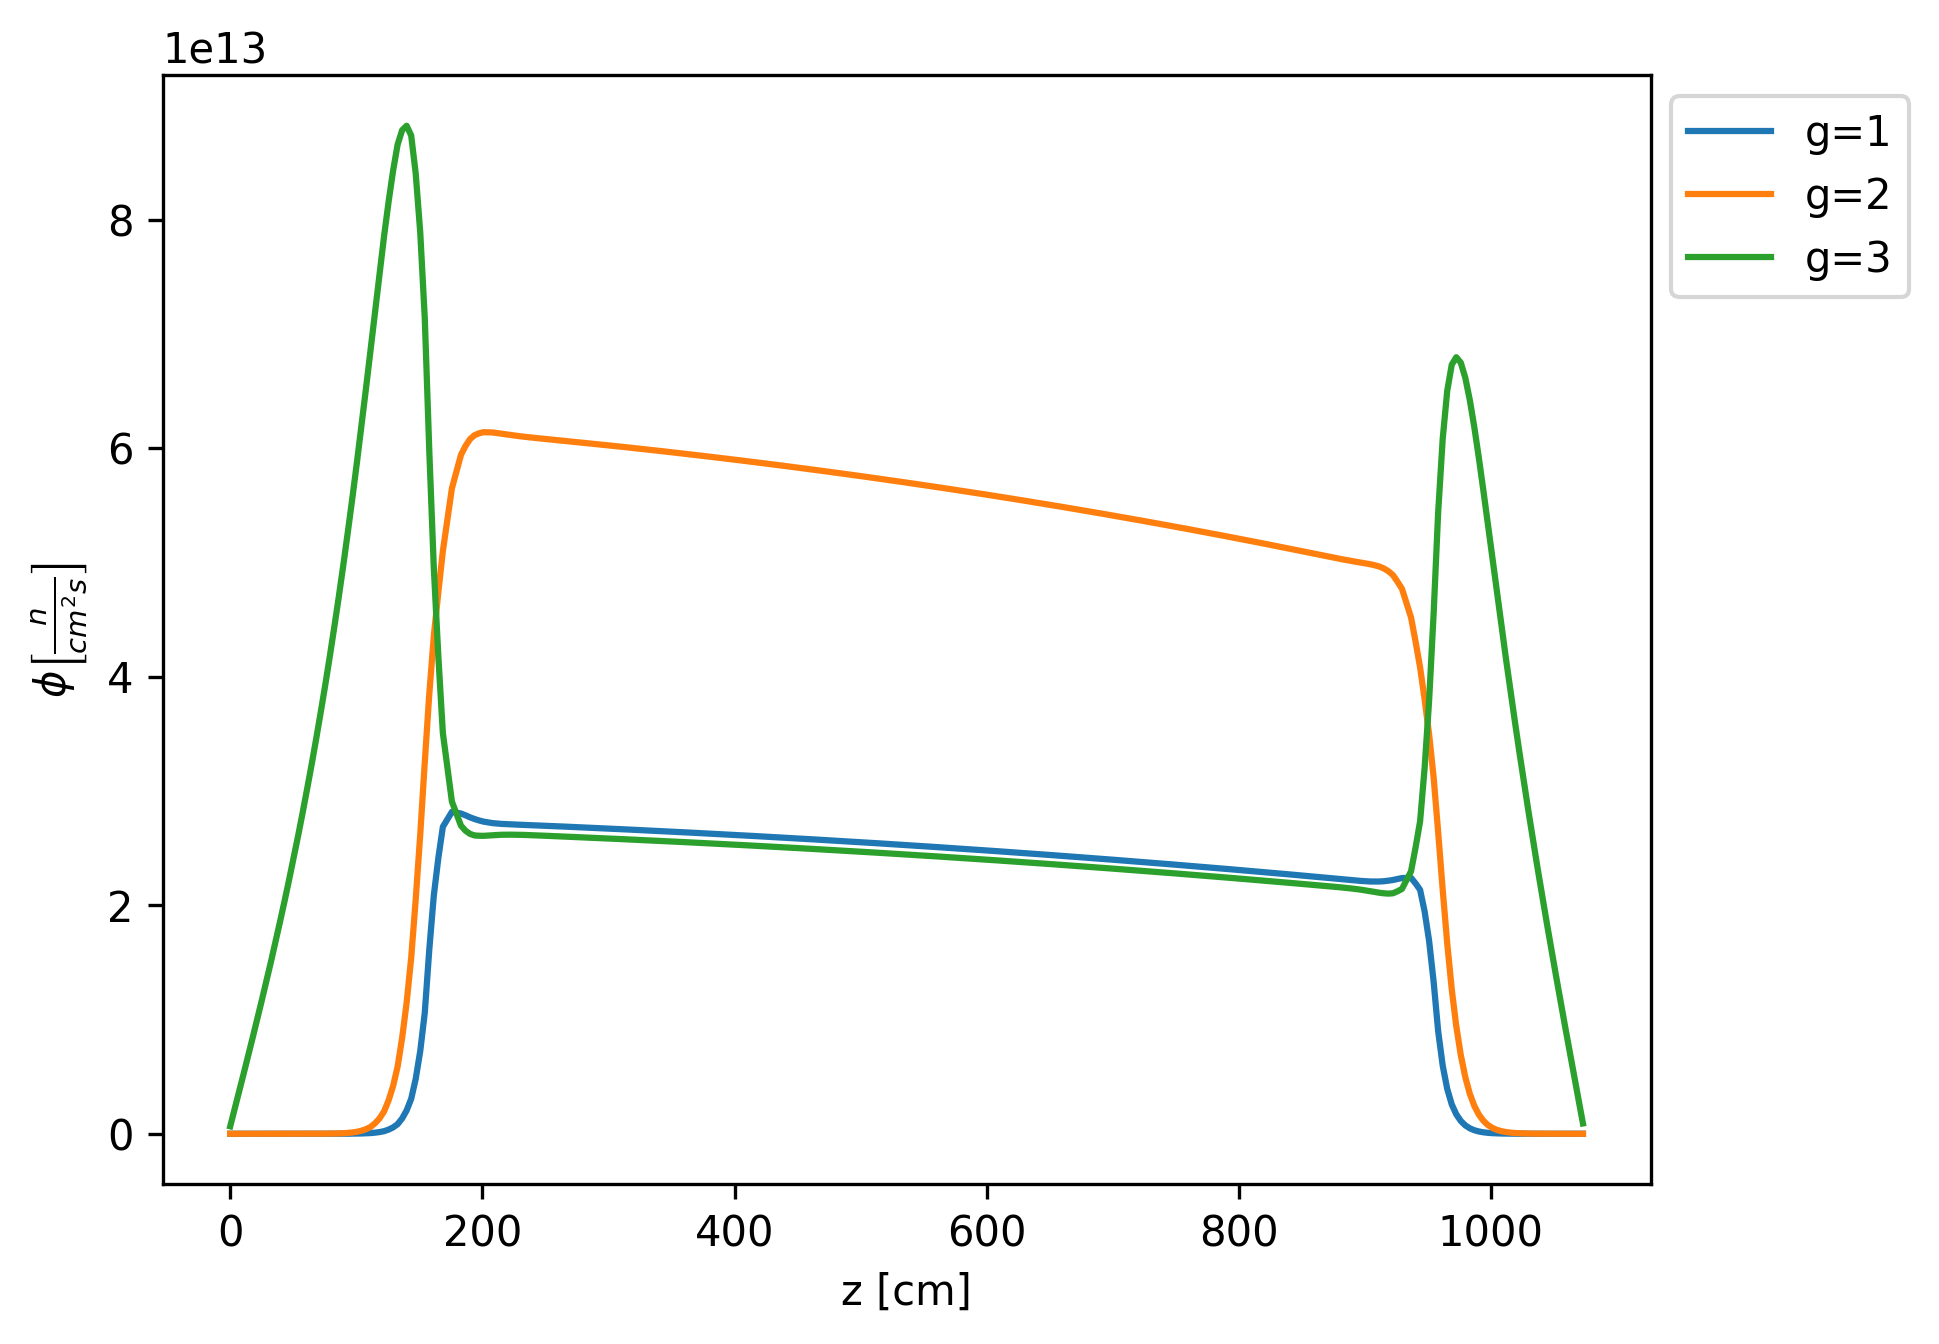
\includegraphics[width=0.45\textwidth]{figures-assembly/3D-assembly-noLBP-1200-26G}
    }
    \subfloat[Serpent.]{
        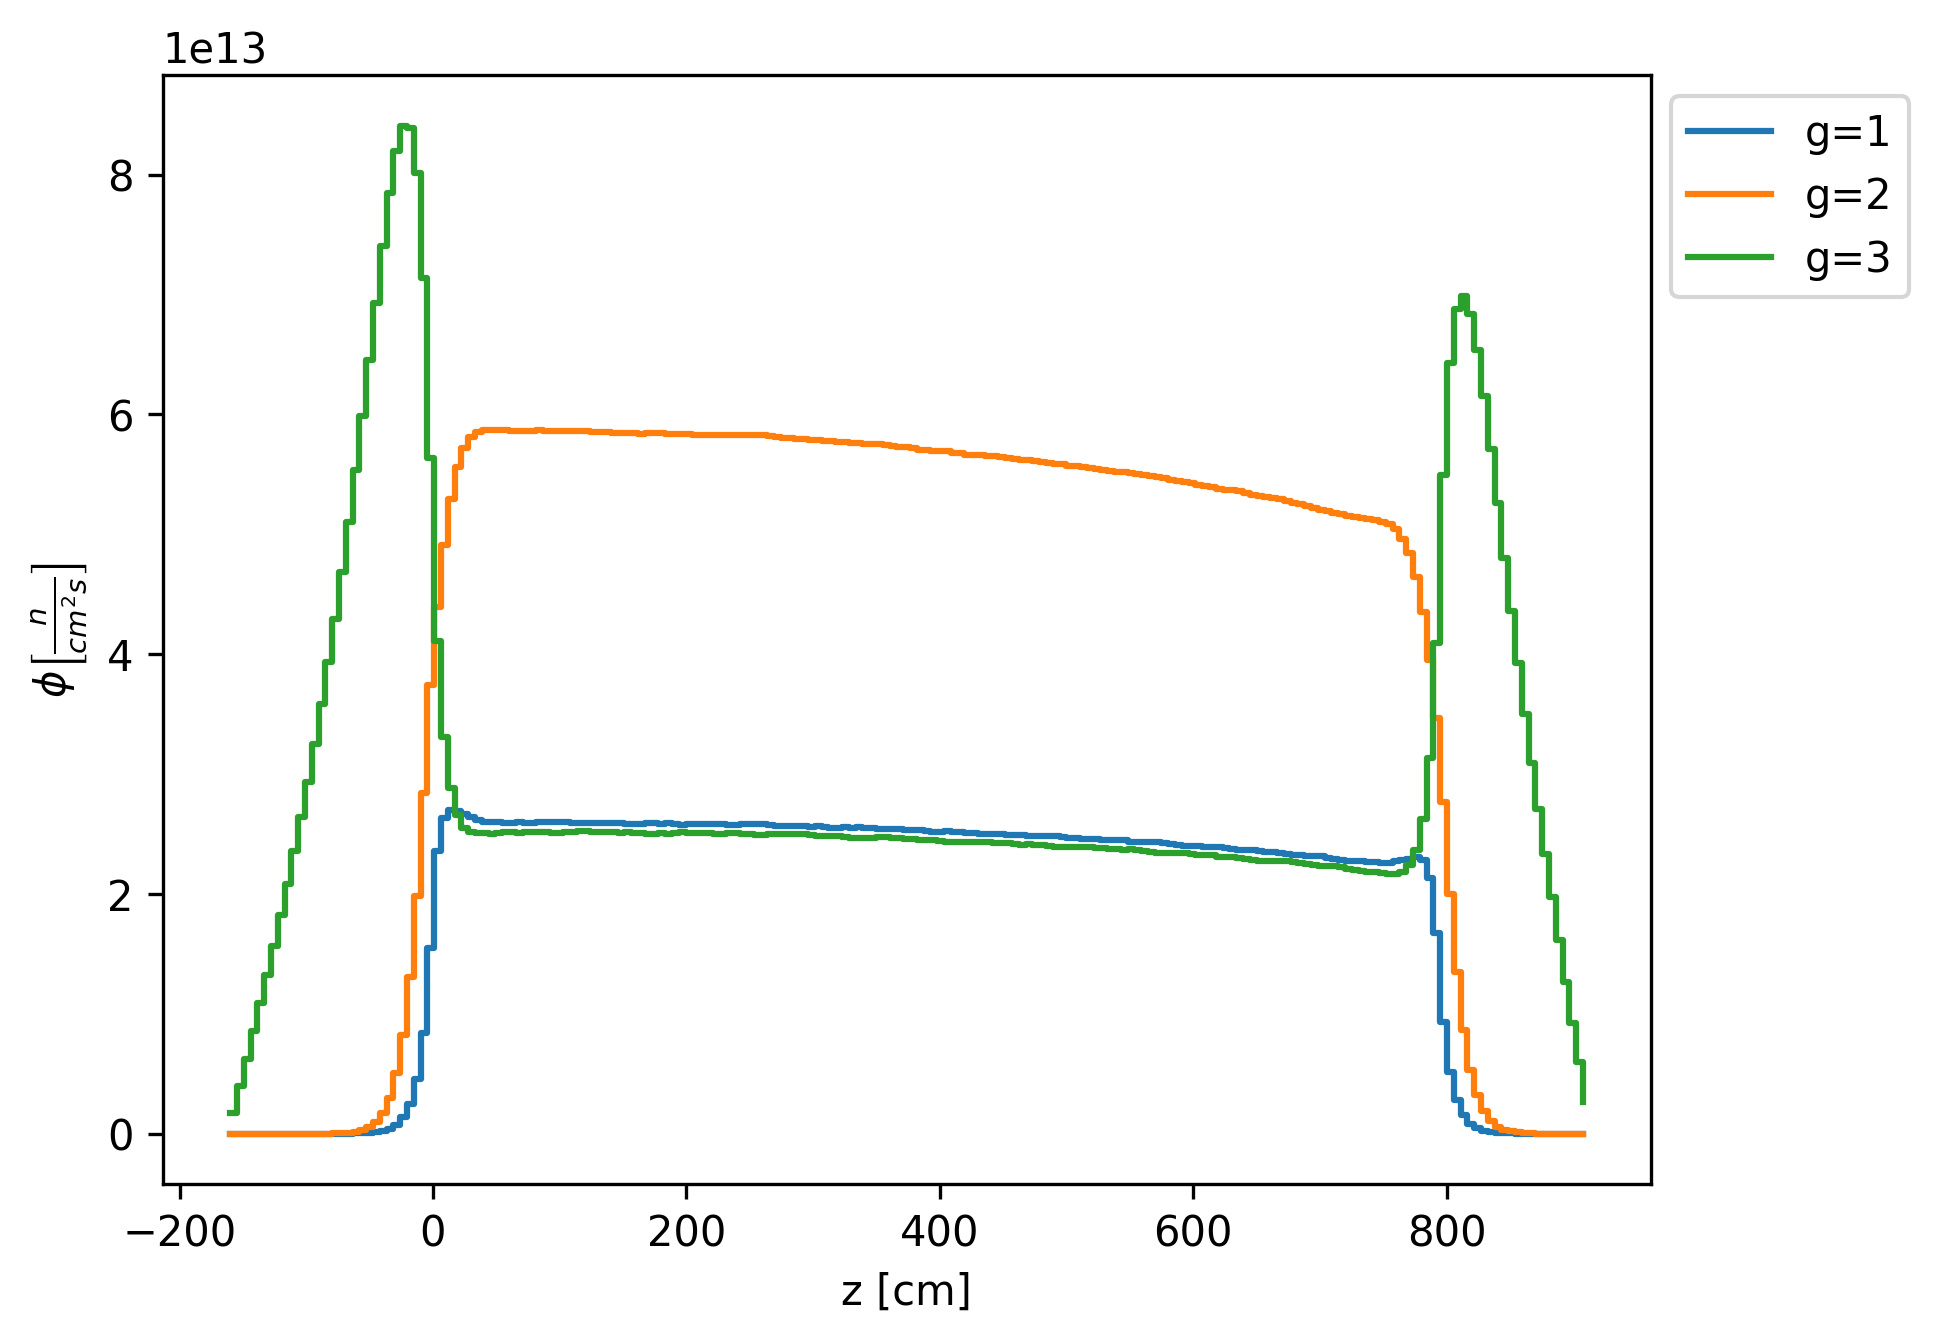
\includegraphics[width=0.45\textwidth]{figures-assembly/serpent26G-noLBP-1200-collapse}
    }
  \hfill
    \caption{Case no LBP at 1200K. 3-group axial neutron flux.}
  \label{fig:assembly-noLBP-1200-flux}
\end{figure}

% LBP 600 
\begin{figure}[htbp!]
  \centering
    \subfloat[Moltres.]{
        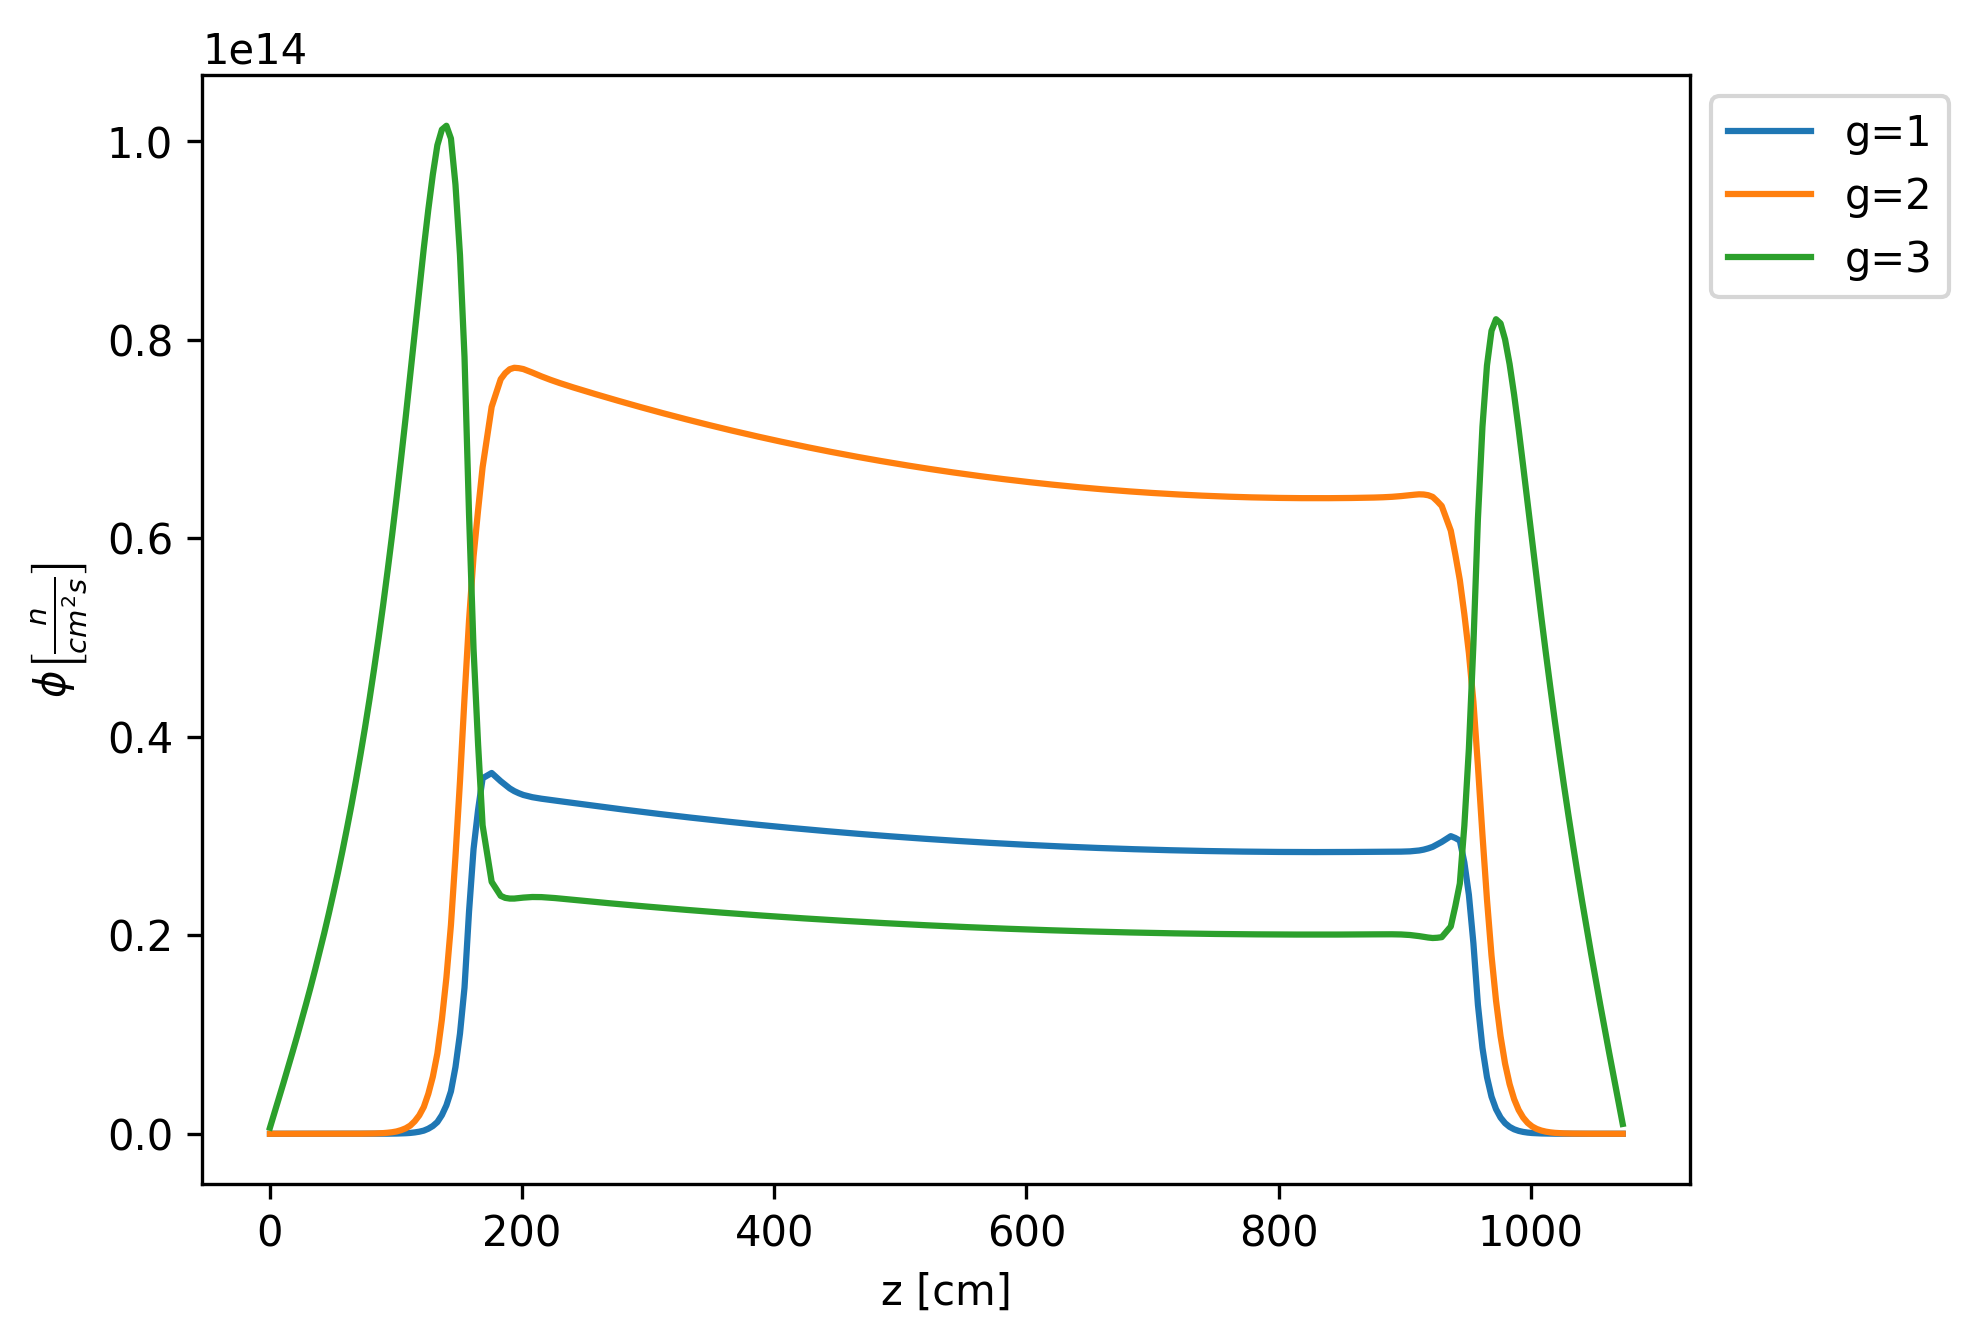
\includegraphics[width=0.45\textwidth]{figures-assembly/3D-assembly-LBP-600-26G}
    }
    \subfloat[Serpent.]{
        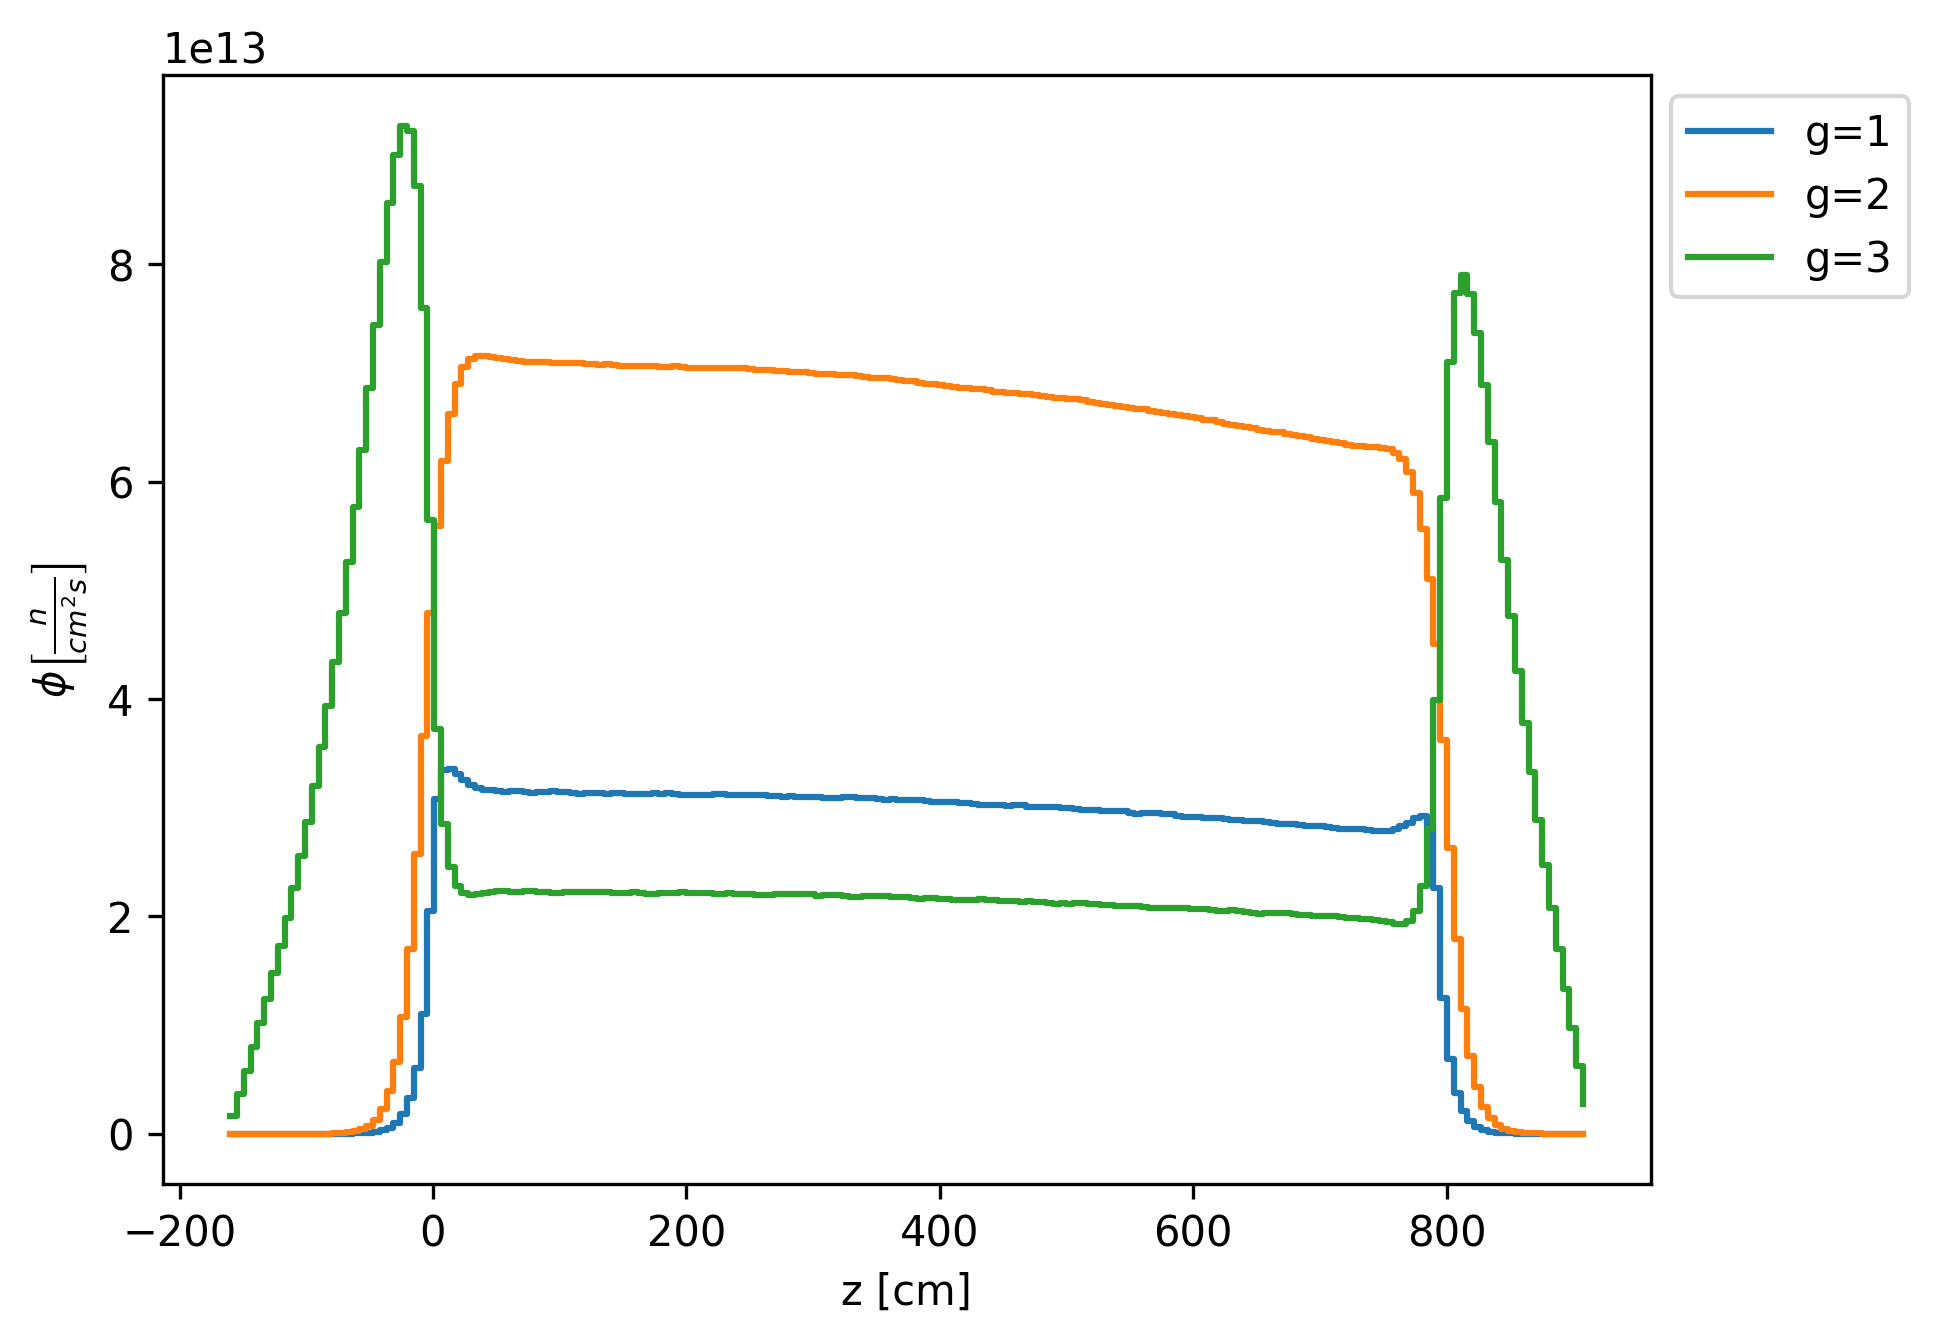
\includegraphics[width=0.45\textwidth]{figures-assembly/serpent26G-LBP-600-collapse}
    }
  \hfill
    \caption{Case LBP at 600K. 3-group axial neutron flux.}
  \label{fig:assembly-LBP-600-flux}
\end{figure}

% LBP 1200
\begin{figure}[htbp!]
  \centering
    \subfloat[Moltres.]{
        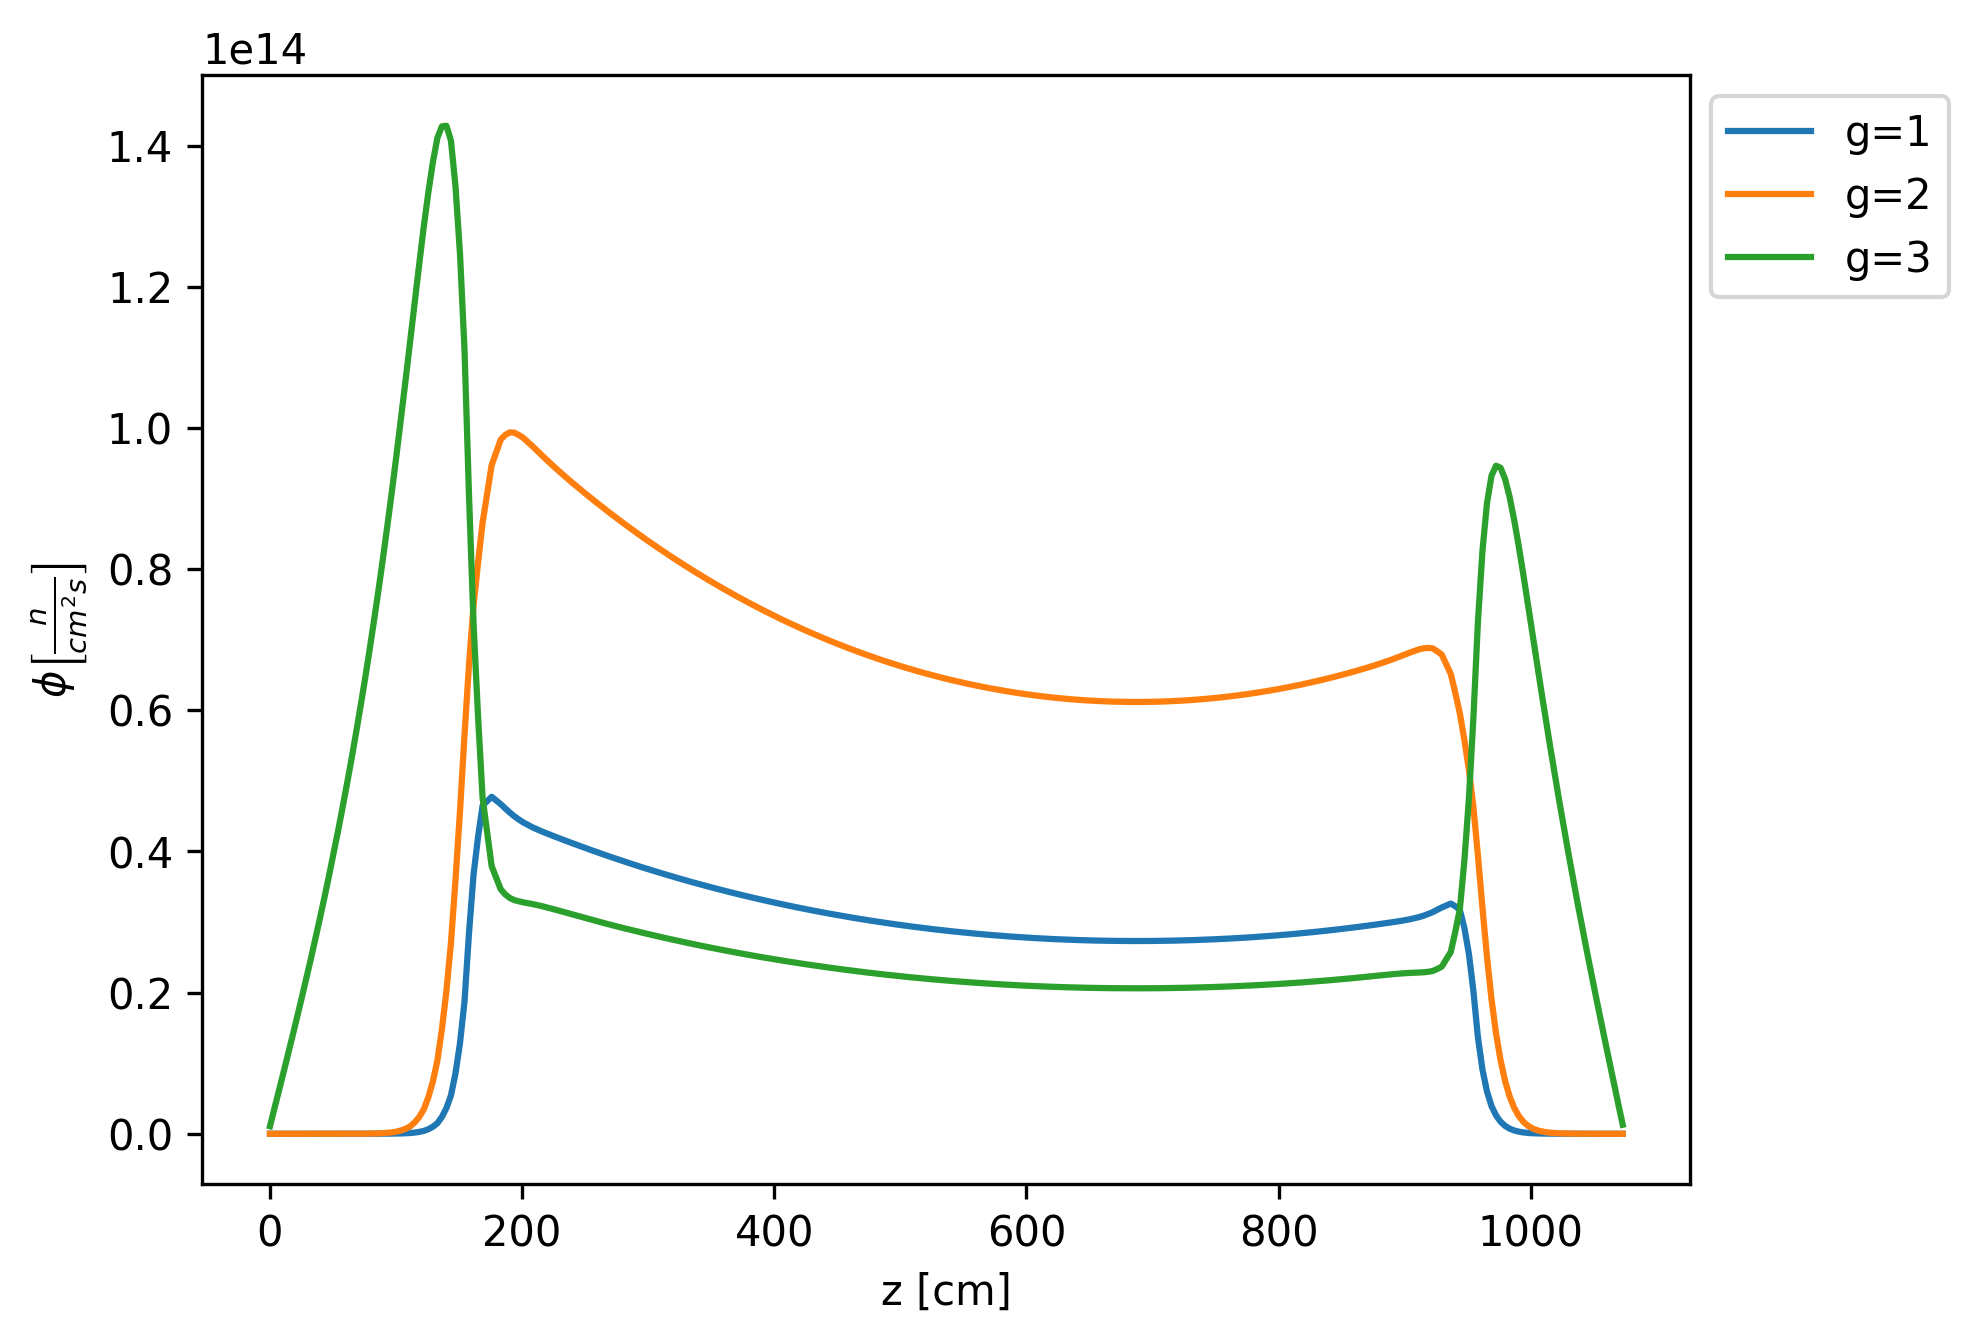
\includegraphics[width=0.45\textwidth]{figures-assembly/3D-assembly-LBP-1200-26G}
    }
    \subfloat[Serpent.]{
        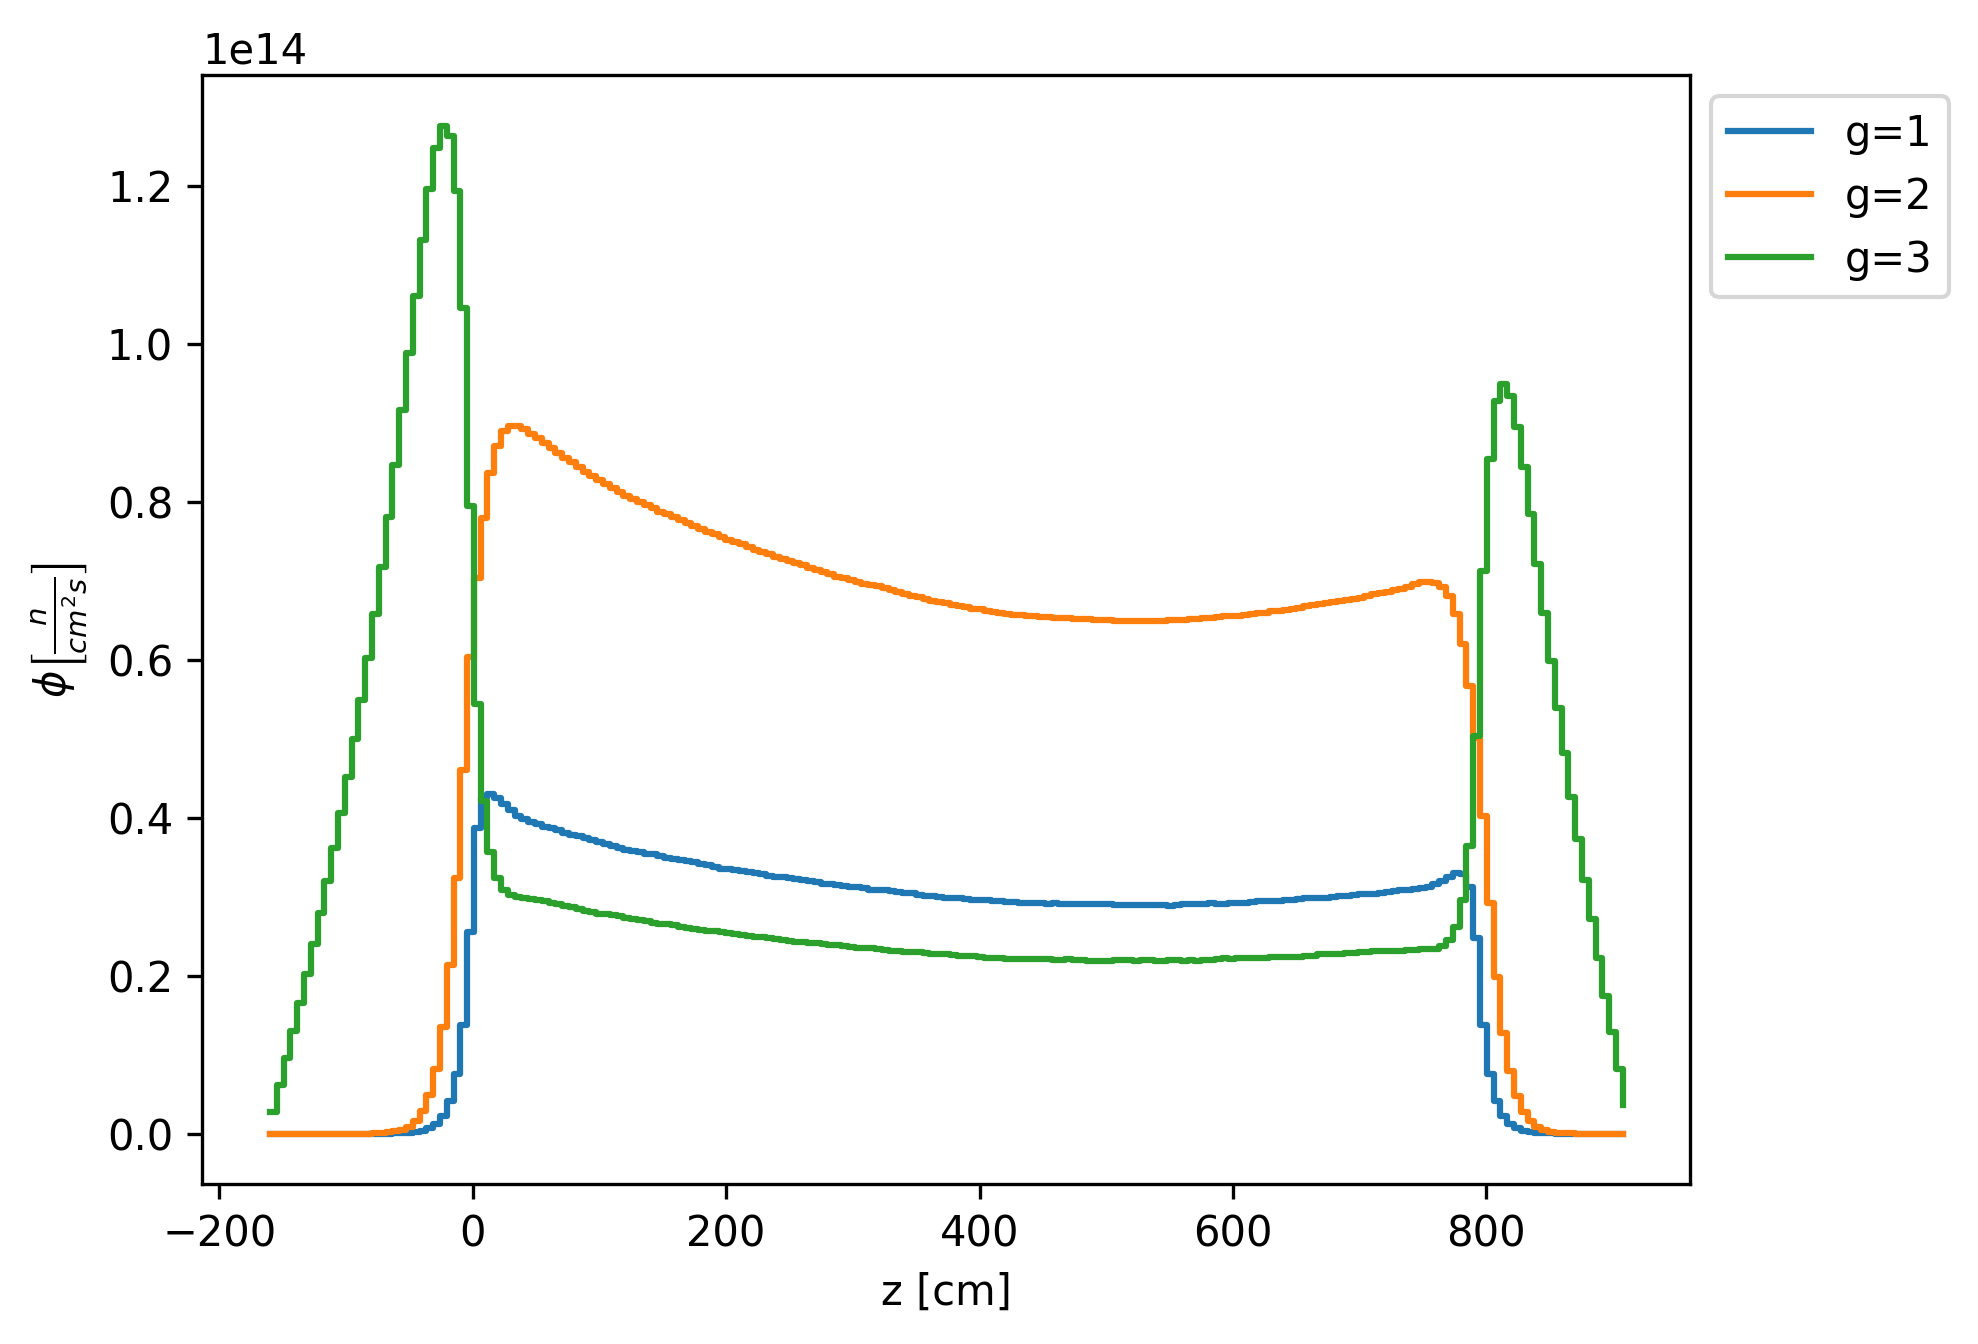
\includegraphics[width=0.45\textwidth]{figures-assembly/serpent26G-LBP-1200-collapse}
    }
  \hfill
    \caption{Case LBP at 1200K. 3-group axial neutron flux.}
  \label{fig:assembly-LBP-1200-flux}
\end{figure}

\begin{table}[htbp!]
  \centering
  \caption{Serpent and Moltres eigenvalues.}
  \begin{tabular}{l|l|llllllll}
  \toprule
              & Serpent 					& \multicolumn{8}{c}{$\Delta \rho$ [pcm]}            \\ \cline{3-10} 
              &              			& 3   & 6   & 9   & 12   & 15   & 18   & 21   & 26   \\
  \midrule
no LBP, 600K  & 1.43800           & 10  & 7   & 6   & 6    & 5    & 6    & 6    & 12   \\
no LBP, 1200K & 1.37771           & 23  & 15  & 4   & 3    & 2    & 2    & 1    & 11   \\
LBP, 600K     & 1.12861           & 44  & 21  & 24  & 25   & 25   & 24   & 19   & 9    \\
LBP, 1200K    & 1.06554           & 36  & 40  & 29  & 32   & 44   & 43   & 25   & 25   \\
  \bottomrule
  \end{tabular}
  \label{tab:keff}
\end{table}

% No LBP
\begin{figure}[htbp!]
	\centering
    \subfloat[600K.]{
        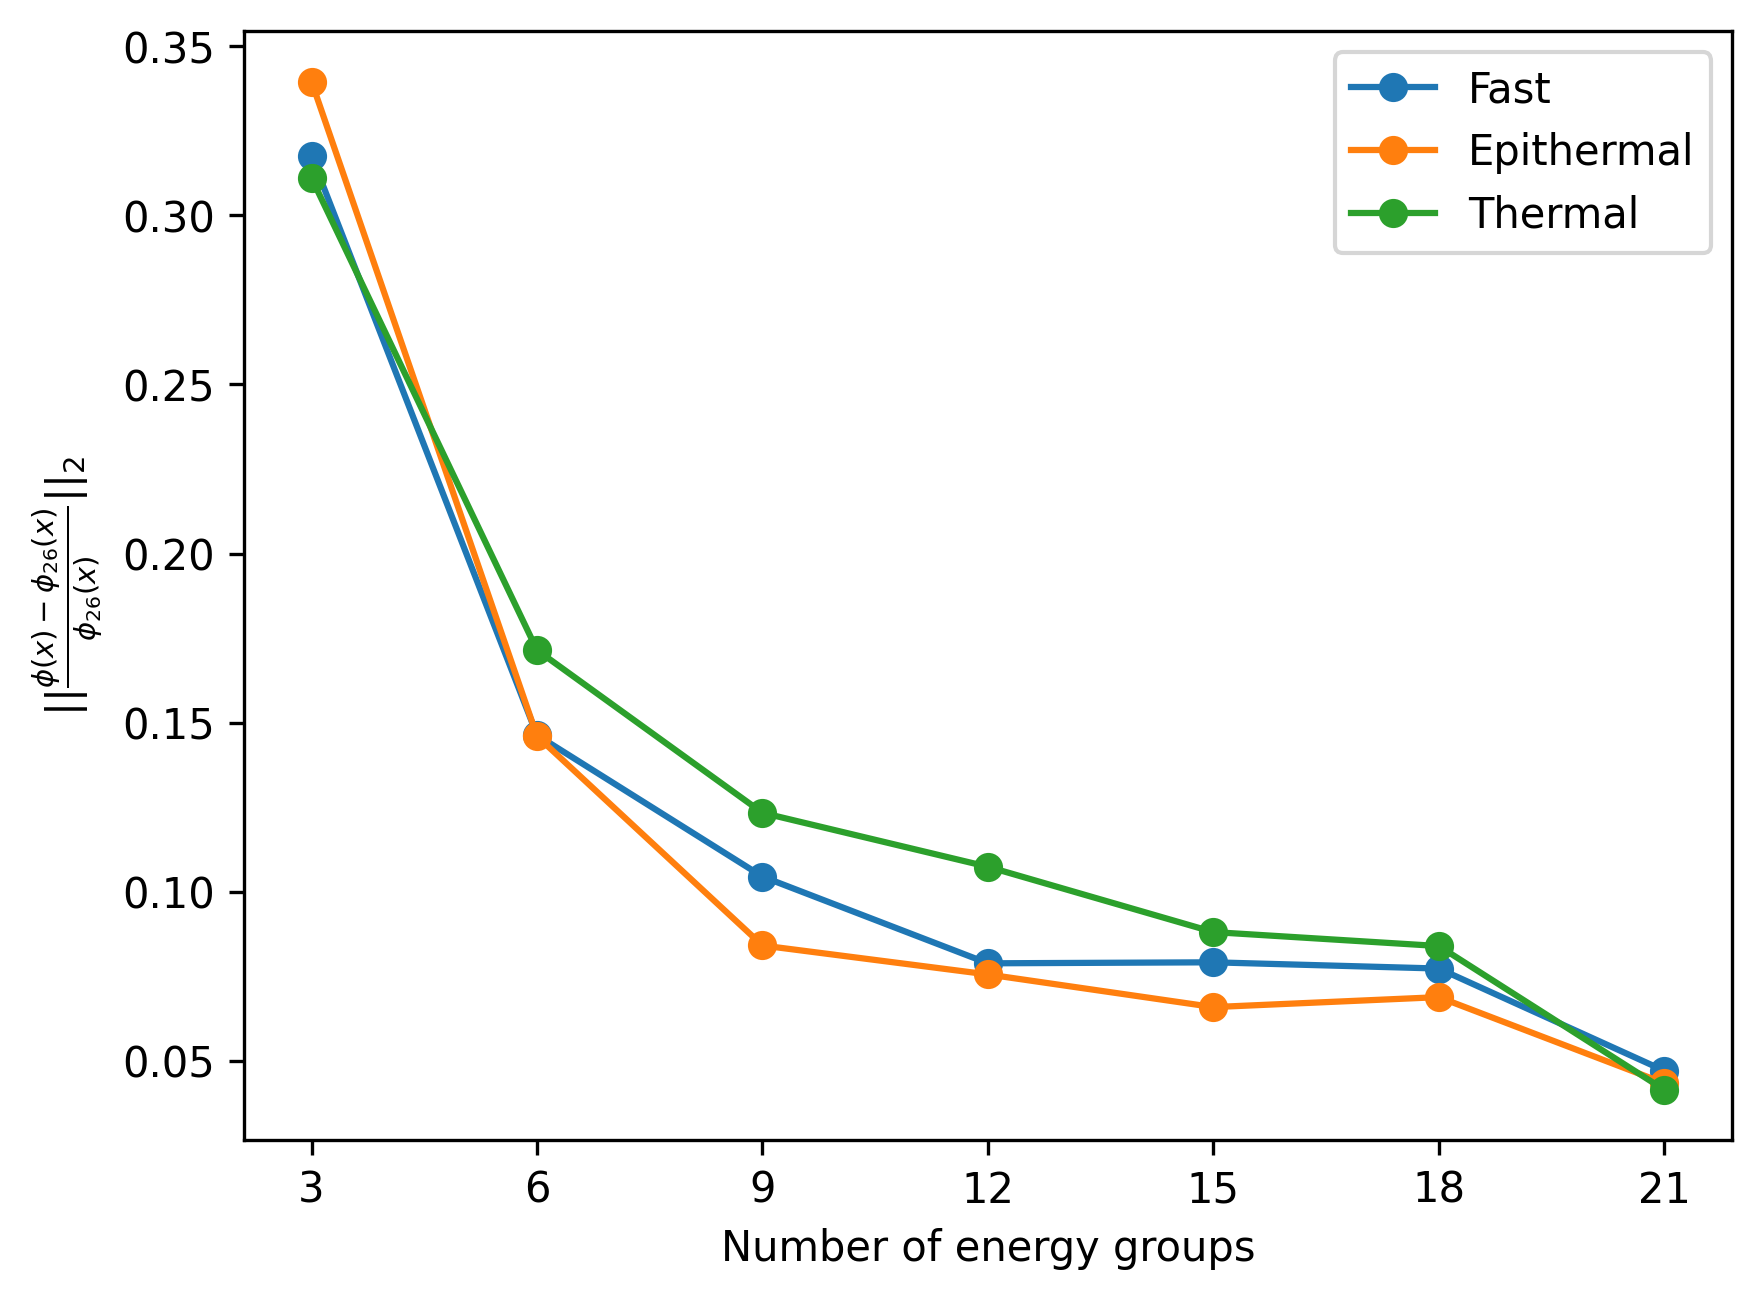
\includegraphics[width=0.45\textwidth]{figures-assembly/noLBP-600-er-final}
    }
    \subfloat[1200K.\label{fig:assembly-noLBP-er-b}]{
        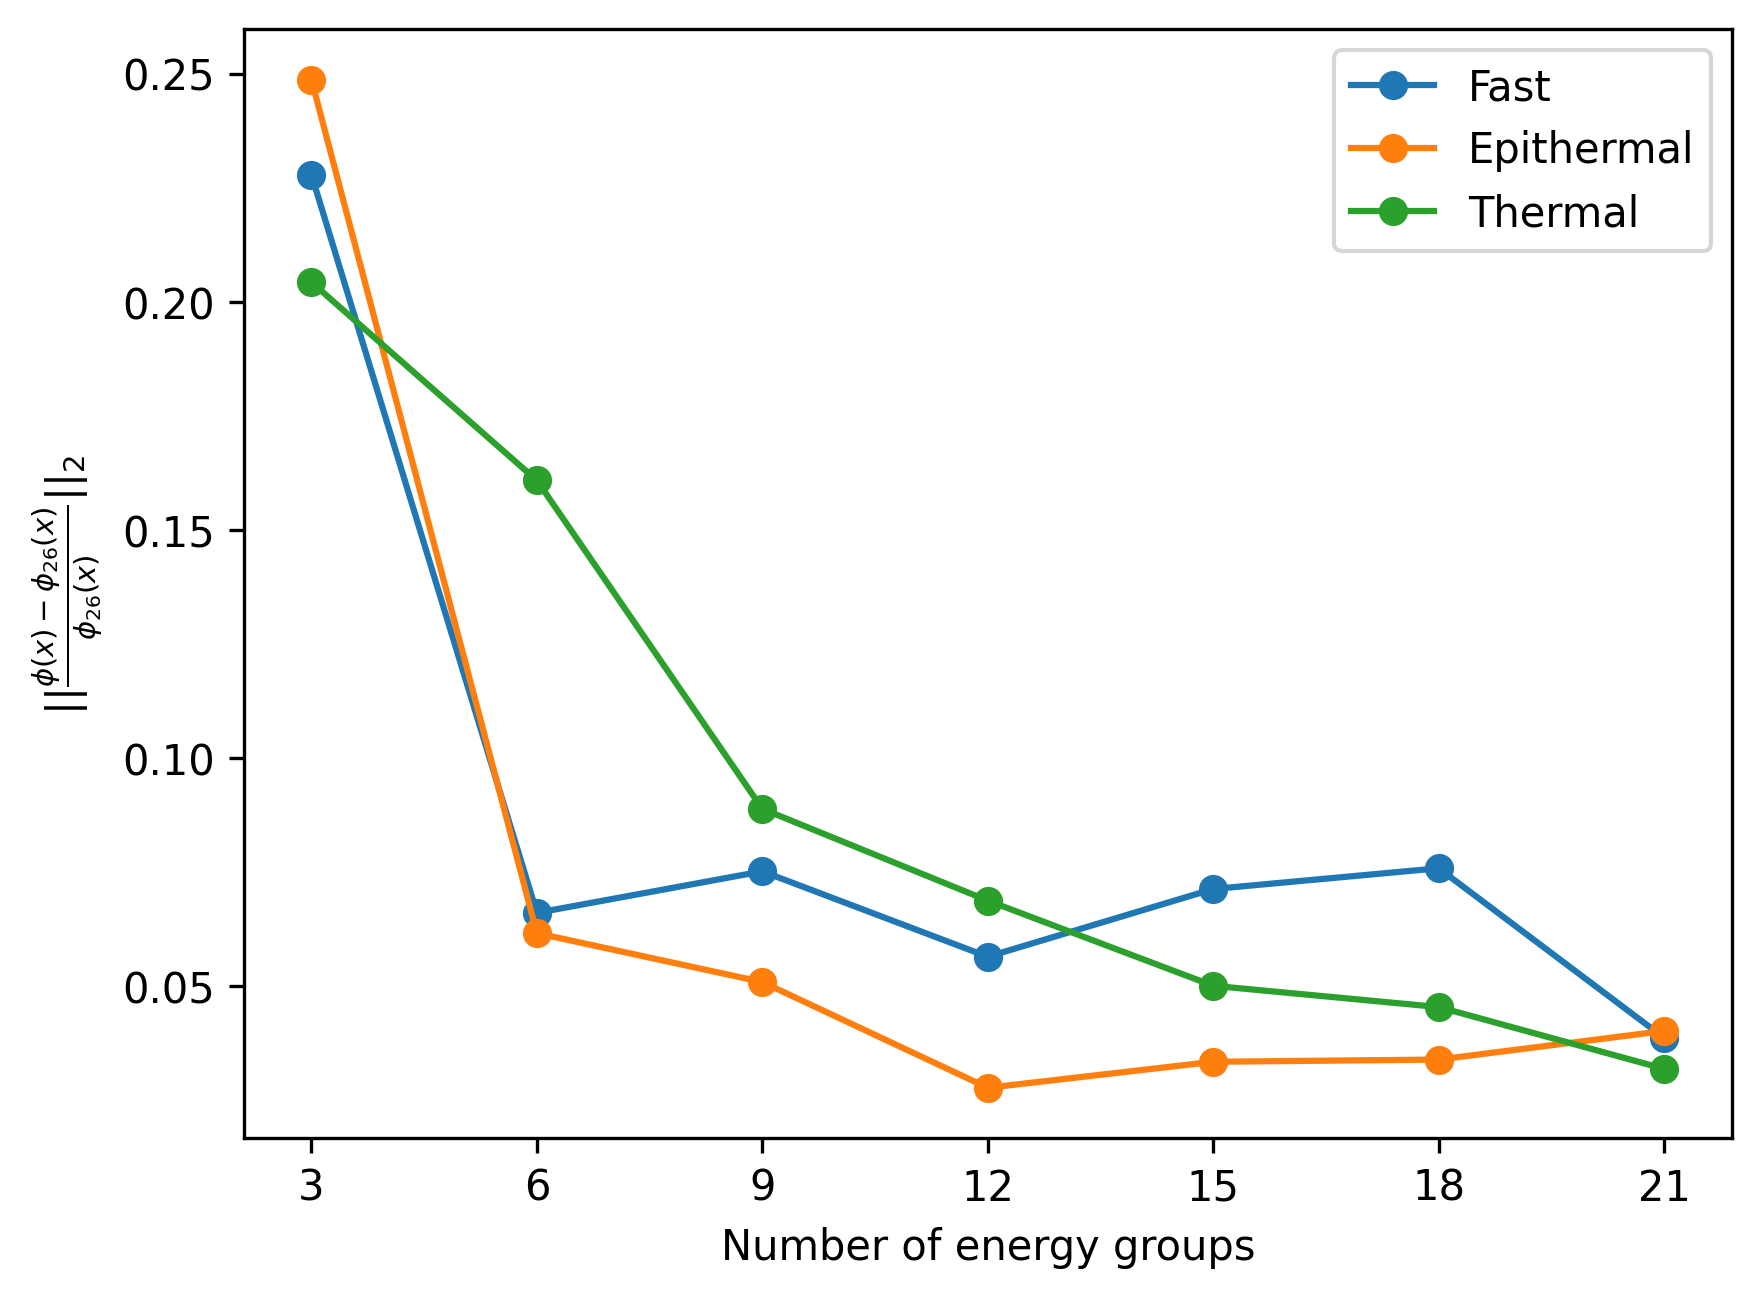
\includegraphics[width=0.45\textwidth]{figures-assembly/noLBP-1200-er-final}
    }
	\hfill
    \caption{No LBP case. L$_2$-norm relative error for different number of energy group structures.}
	\label{fig:assembly-noLBP-er}
\end{figure}

% LBP
\begin{figure}[htbp!]
	\centering
    \subfloat[600K.]{
        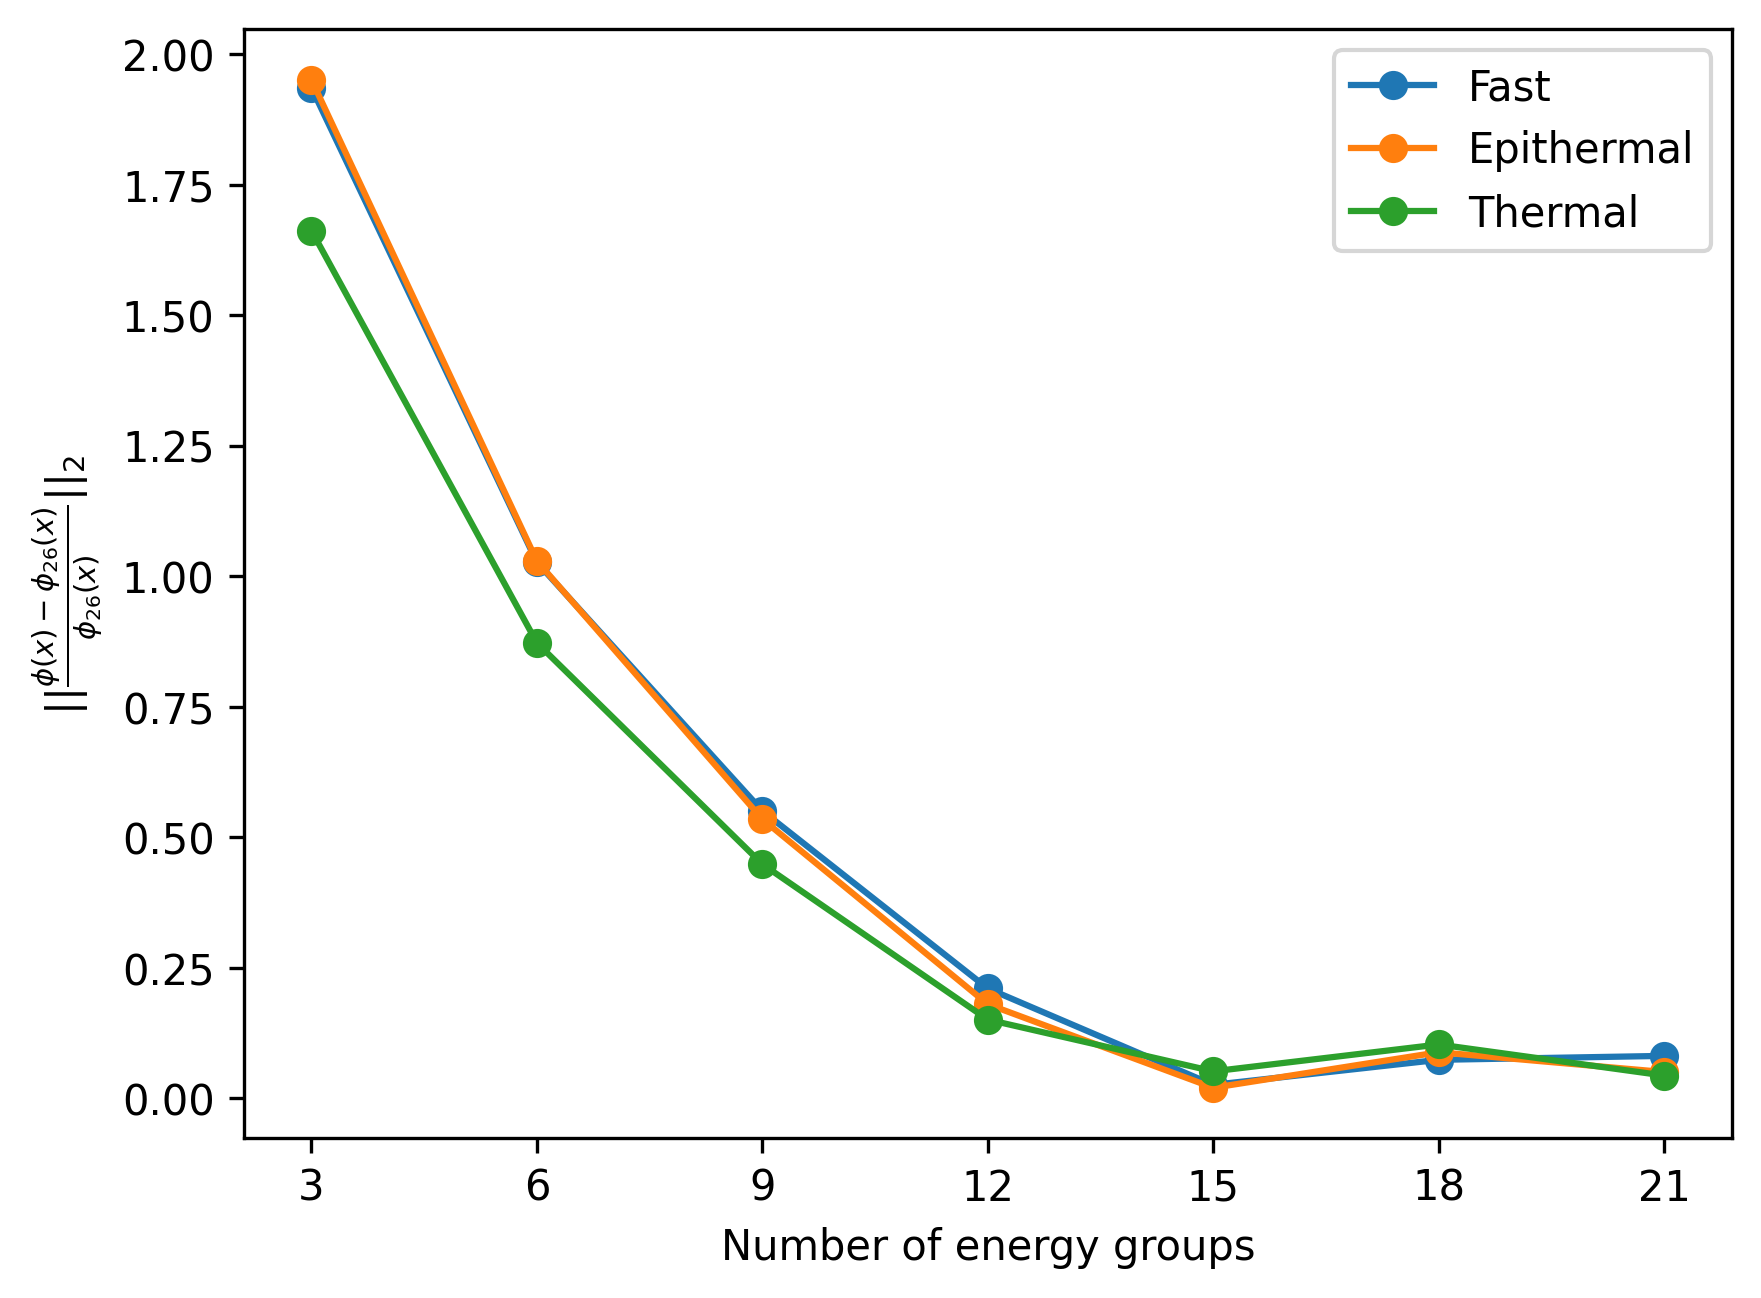
\includegraphics[width=0.45\textwidth]{figures-assembly/LBP-600-er-final}
    }
    \subfloat[1200K.]{
        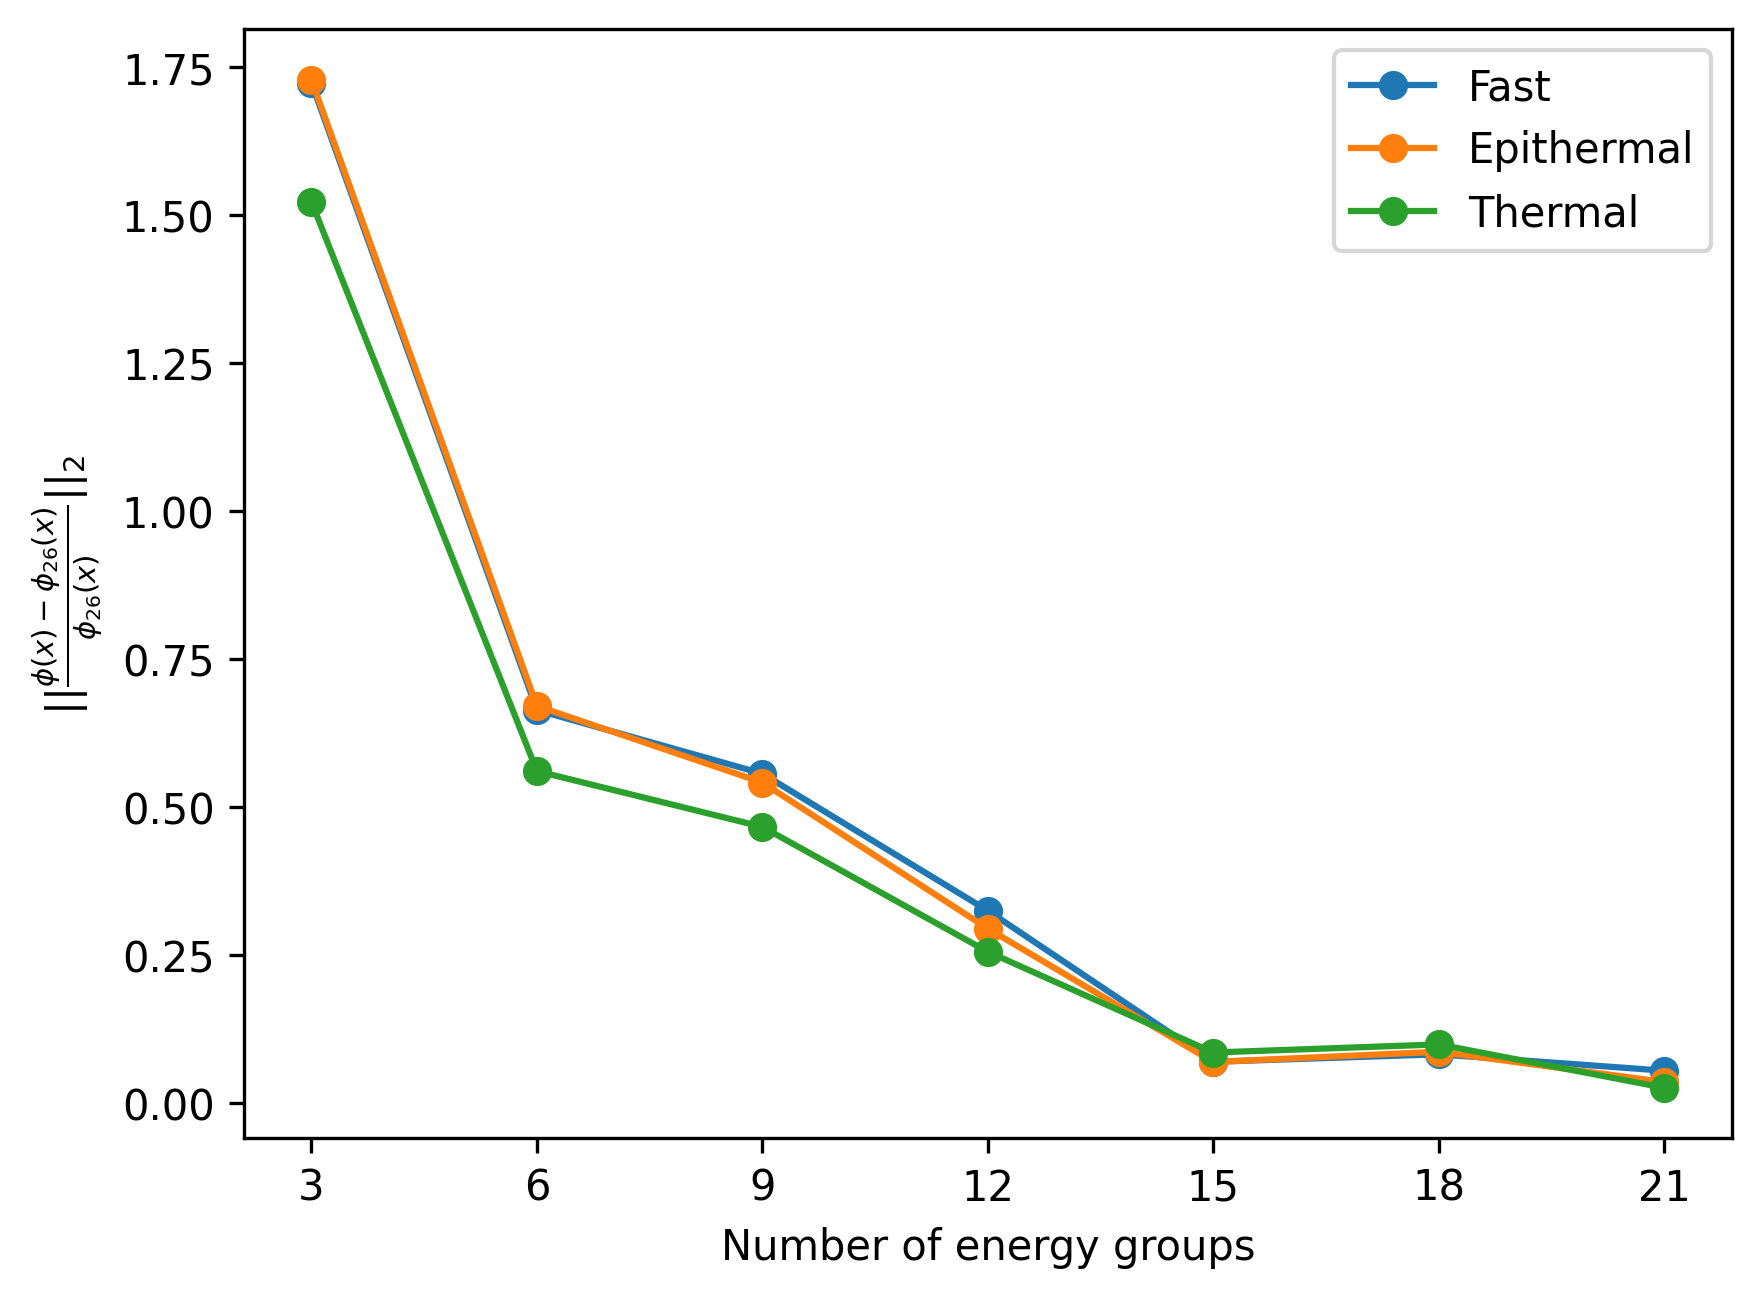
\includegraphics[width=0.45\textwidth]{figures-assembly/LBP-1200-er-final}
    }
	\hfill
    \caption{LBP case. L$_2$-norm relative error for different number of energy group structures.}
	\label{fig:assembly-LBP-er}
\end{figure}

% Time and memory
\begin{figure}[htbp!]
	\centering
    \subfloat[No LBP and 600 K.]{
        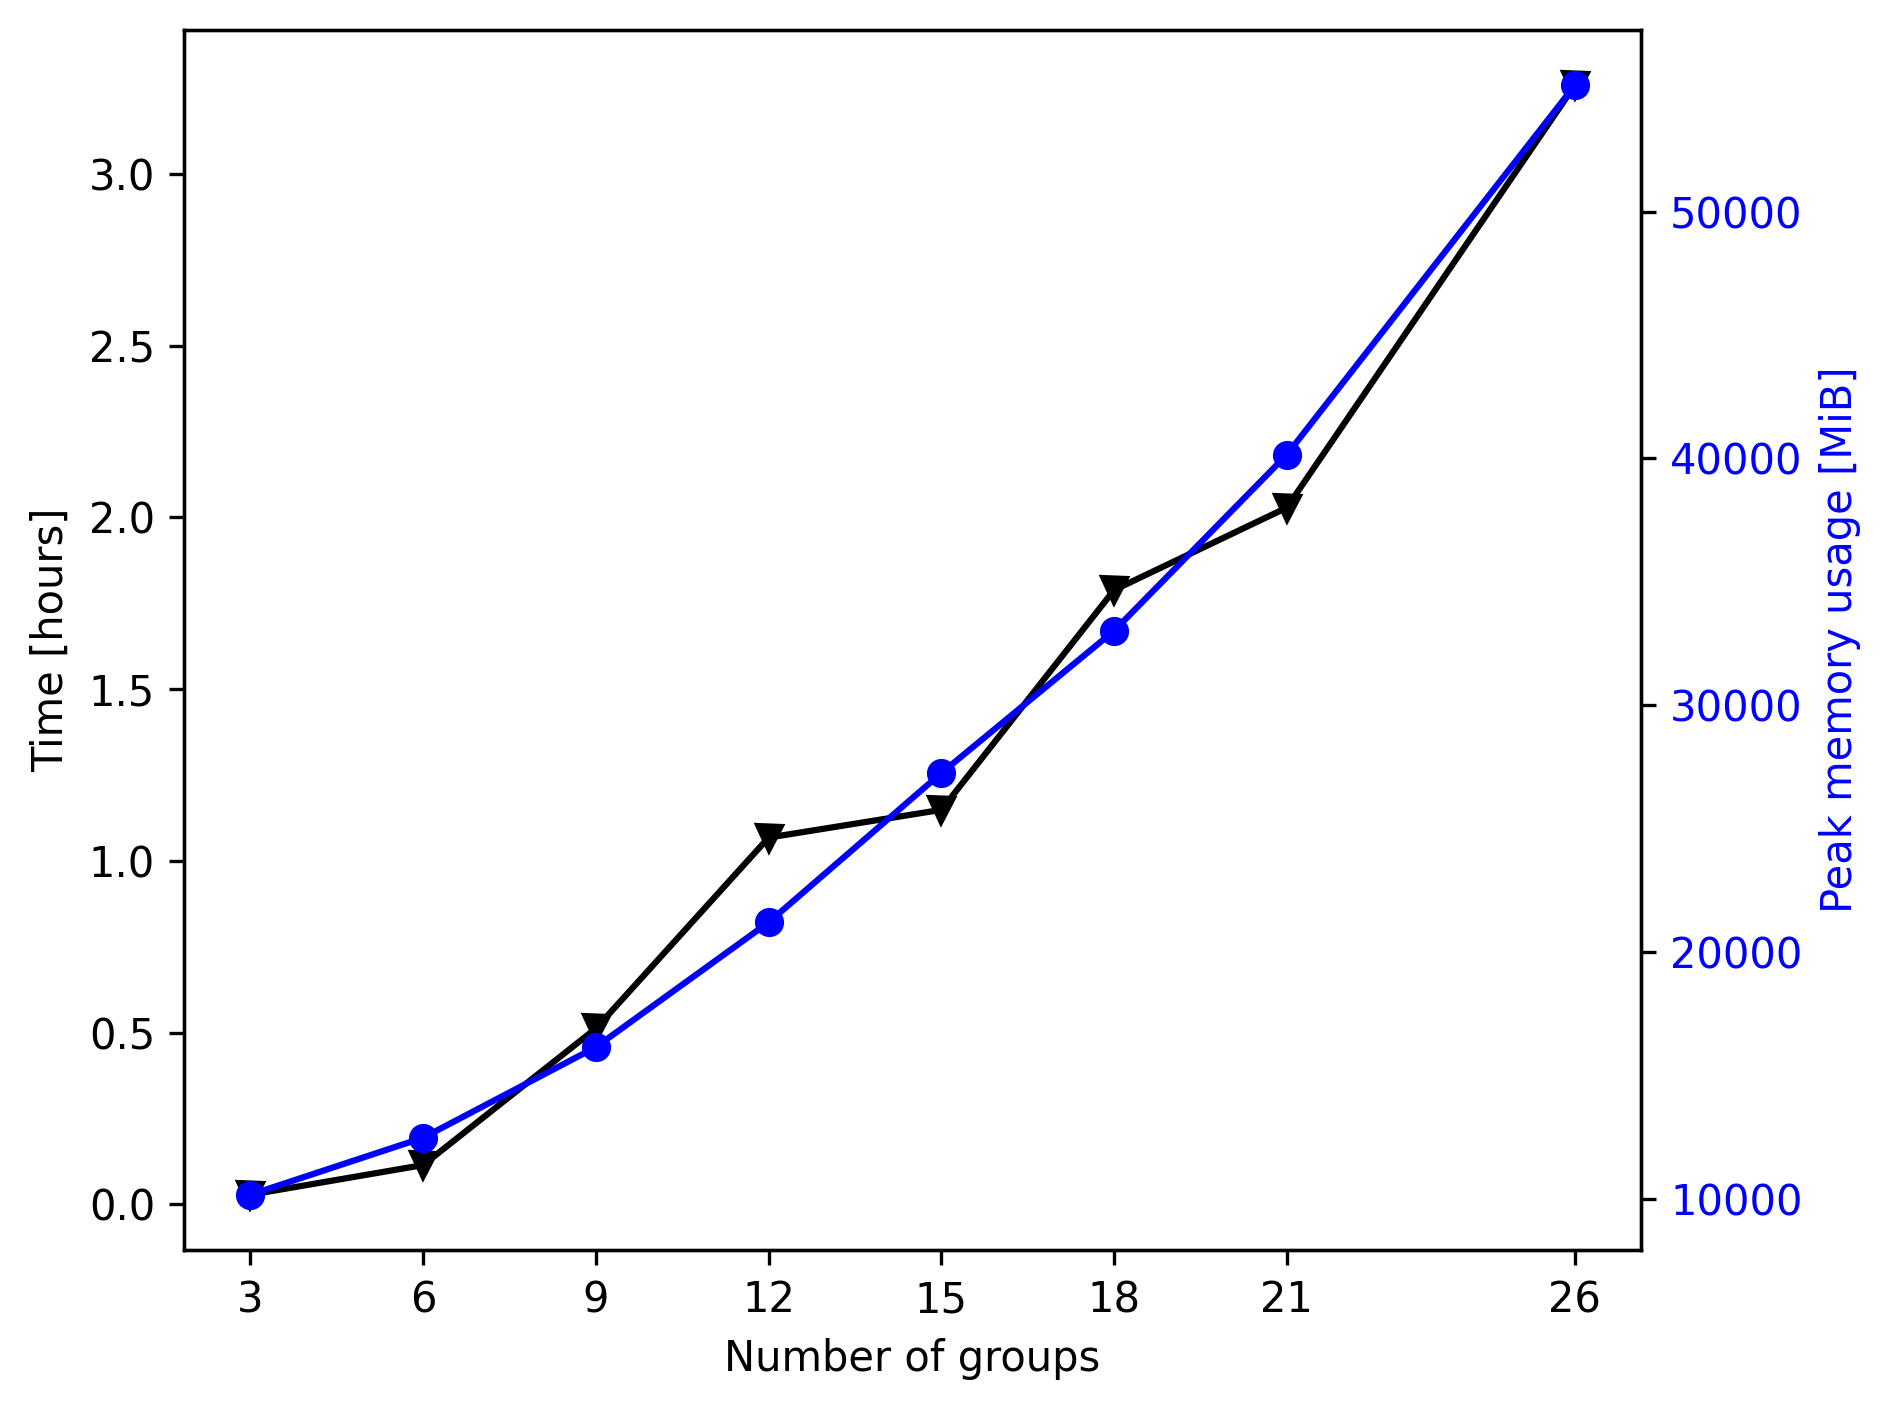
\includegraphics[width=0.45\textwidth]{figures-assembly/time-noLBP-600}
    }
    \subfloat[LBP and 600 K.]{
        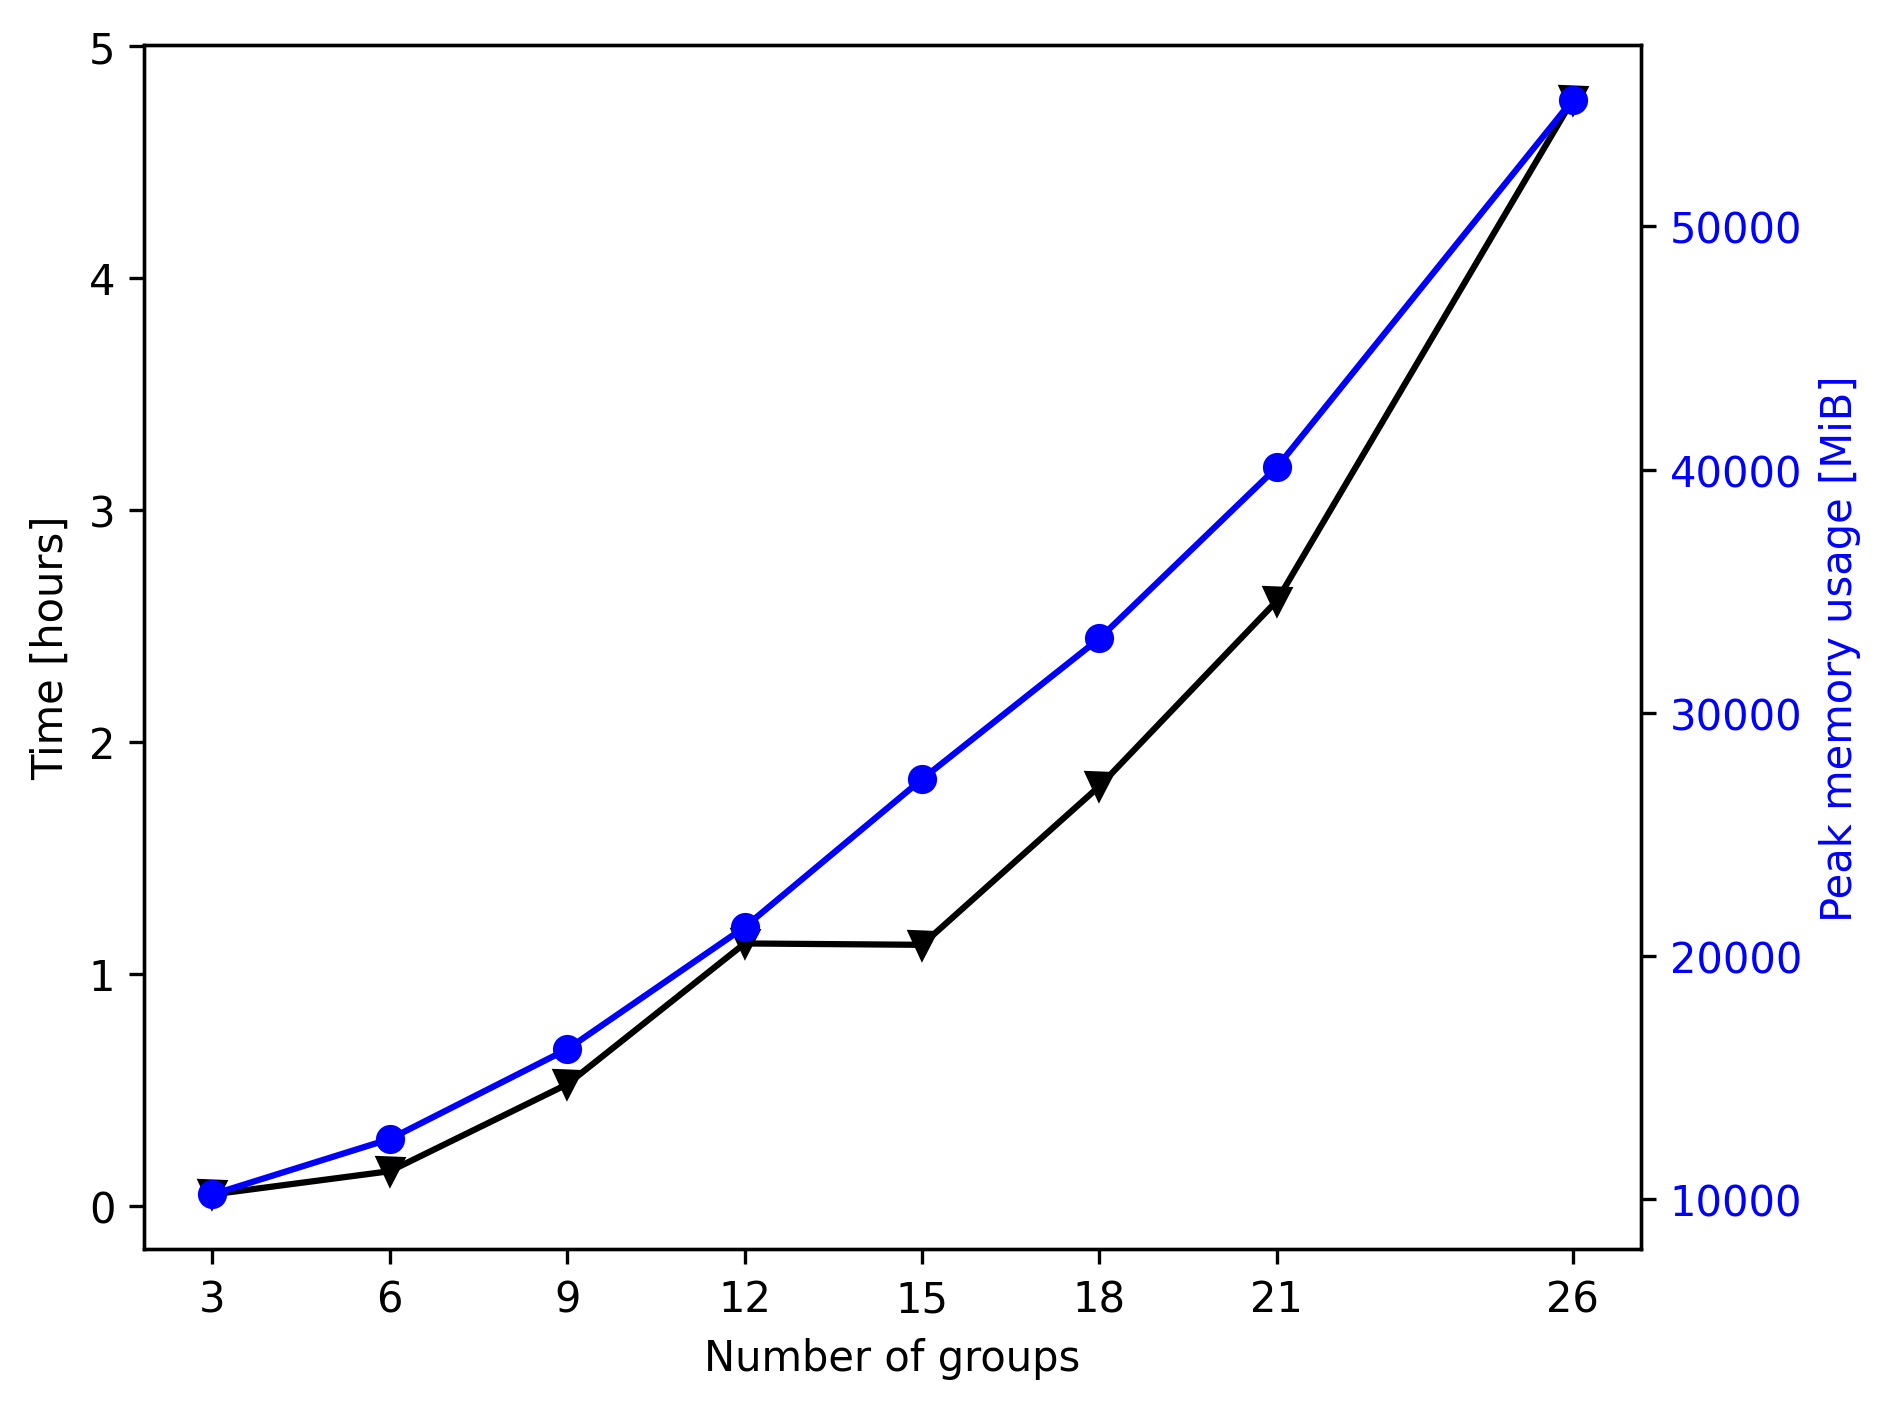
\includegraphics[width=0.45\textwidth]{figures-assembly/time-LBP-600}
    }
	\hfill
	\caption{Computational time and memory requirements for different number of energy group structures.}
	\label{fig:assembly-time}
\end{figure}

\begin{table}[htbp!]
  \centering
  \caption{$L_2$-norm relative error for various energy group structures. Values expressed in percentage.}
  \begin{tabular}{@{}l|l|l| S[table-format=2.1] S[table-format=2.1] S[table-format=2.1] S[table-format=2.1] S[table-format=2.1] }
  \toprule
	LBP                  & Temperature {[}K{]}   & Flux       & \multicolumn{1}{c@{}}{15a} & \multicolumn{1}{c@{}}{15b}  & \multicolumn{1}{c@{}}{15c}  & \multicolumn{1}{c@{}}{15d}  & \multicolumn{1}{c@{}}{15e}  \\
	\midrule
	\multirow{6}{*}{No}  & \multirow{3}{*}{600}  & Fast       & 7.9  & 8.0  & 8.2  & 8.1  & 9.1  \\
	                     &                       & Epithermal & 6.6  & 6.5  & 8.6  & 8.2  & 9.2  \\
	                     &                       & Thermal    & 8.8  & 8.5  & 10.6 & 10.7 & 12.9 \\ \cline{2-8}
	                     & \multirow{3}{*}{1200} & Fast       & 7.1  & 7.7  & 5.7  & 5.1  & 4.5  \\
	                     &                       & Epithermal & 3.3  & 3.9  & 6.2  & 5.1  & 3.4  \\
	                     &                       & Thermal    & 5.0  & 4.7  & 8.5  & 8.2  & 8.4  \\ \hline
	\multirow{6}{*}{Yes} & \multirow{3}{*}{600}  & Fast       & 24.0 & 24.8 & 2.6  & 2.3  & 3.7  \\
	                     &                       & Epithermal & 21.0 & 21.7 & 2.0  & 1.6  & 2.7  \\
	                     &                       & Thermal    & 18.1 & 18.8 & 5.2  & 5.5  & 5.7  \\ \cline{2-8}
	                     & \multirow{3}{*}{1200} & Fast       & 36.2 & 37.3 & 6.9  & 6.6  & 25.9 \\
	                     &                       & Epithermal & 33.2 & 34.2 & 6.9  & 6.5  & 25.1 \\
	                     &                       & Thermal    & 29.6 & 30.6 & 8.5  & 8.3  & 20.3 \\
	\midrule
	\multicolumn{2}{l}{Weighted average}         &            & 17.3 & 17.8 & 6.3  & 6.0  & 10.8 \\
	\bottomrule
  \end{tabular}
  \label{tab:accuracy15}
\end{table}


\subsection{Full-core}

In this section, we compared the results from Serpent and Moltres for a full-core simulation.
The first step in the calculation was to obtain the group constants using Serpent.
Figure \ref{fig:fullcoremodel} displays the $xy$-plane of the model.
The model includes the bottom and top reflectors.
Tables \ref{tab:maincharac}, \ref{tab:element-characteristics} and \ref{tab:compact} specify the model input parameters.
To simplify Serpent's model, all the fuel columns were standard fuel columns.
Additionally, the model does not include the fuel handling holes nor the coolant channels in the bottom and top reflectors.
The model considered a fresh core.
Based on the previous section analyses, we chose the energy group structure $15d$ in Table \ref{tab:energygroups}.
The material temperatures were 600K and 1200K, cases that represent the \gls{CZP} and the \gls{HFP} core states.
Serpent ran 8$\times 10^5$ neutrons/cycle, 500 active cycles, and 100 inactive cycles for the calculations.

For the Moltres input file, we made the geometry and mesh using Gmsh.
Taking advantage of the symmetry of the problem, the model included only a one-sixth of the full-core.
The mesh had 300720 elements and 160035 nodes.
The diffusion calculations had 160035 \glspl{DoF}/energy-group, and a total of 2400525 DoFs.
The Moltres input files set an eigenvalue and a flux convergence tolerance of 1$\times$10$^{-8}$.

% Keff
Between Serpent and Moltres, we compared the \gls{Keff}, the power distribution, and the flux shape and magnitude in different zones of the reactor.
Table \ref{tab:full-keff} exhibits the \gls{Keff} from Serpent and Moltres.
Moltres values are larger than Serpent's.
The values are within a 300 pcm difference.

% Power distribution
Figures \ref{fig:fullcore-600-power} and \ref{fig:fullcore-1200-power} show Serpent and Moltres radial power distributions.
The following analysis applies for both temperatures.
The first thing that came to our attention is the symmetry of the power distribution.
The results are symmetric with respect to a 60$^{\circ}$ line.
This result suggests that we could reduce the mesh size by a half by considering only a one-twelfth of the reactor.
The next observation is that Moltres exhibits a higher power density than Serpent in the inner ring and outer rings.
The power density in the middle ring is lower for Moltres case.
The largest difference is in the inner ring.
Overall, the results differ in less than 0.30 MW.

% Fluxes
To compare the fluxes, we placed an axial and a radial flux detectors in arbitrary regions of the reactor.
Figure \ref{fig:fullcore-detectors} shows the location of the detectors.
Note that the flux in Serpent is an average over the volume, while the flux in Moltres is the point-wise flux over a line.
The Serpent axial detector's volume was the fuel column's volume.
The Moltres axial detector's location was the center of the fuel column.
The Serpent radial detector's volume had a 2$^{\circ}$-angle and a fuel assembly's height.
Both Serpent and Moltres radial detector's location was the middle of the active core's height.
Moltres ran the calculations for 15 energy groups, and collapsed the results to three groups to facilitate the visualization of the results.
Figures \ref{fig:fullcore-600-axial1} and \ref{fig:fullcore-600-radial1} show the axial and radial fluxes at 600K.
In Figure \ref{fig:fullcore-600-axial1}, the fast and epithermal fluxes in Moltres are larger while the thermal flux is smaller.
The flux shapes are similar.
The epithermal and thermal fluxes are closer in magnitude in the active core in Serpent's simulation.
In Figure \ref{fig:fullcore-600-radial1}, Serpent fluxes present some 'noise'.
A higher number of generations/cycle in Serpent simulations would solve it.
Another alternative is using a detector with a larger volume.
Additionally, the flux in Serpent shows the location of the LBPs in the fuel assemblies.
A diffusion solver fails to capture such localized effects as the group constants are homogeneous in the fuel assembly.
Regarding the magnitude, the fast flux in Moltres is larger while the epithermal and thermal fluxes have almost the same magnitudes.
Figures \ref{fig:fullcore-1200-axial1} and \ref{fig:fullcore-1200-radial1} display the fluxes at 1200K.
These results are different from the 600K case.
However, we observe the same behavior for both axial and radial fluxes.

% Geometries
\begin{figure}[htbp!]
	\centering
    \subfloat[Serpent model geometry.]{
        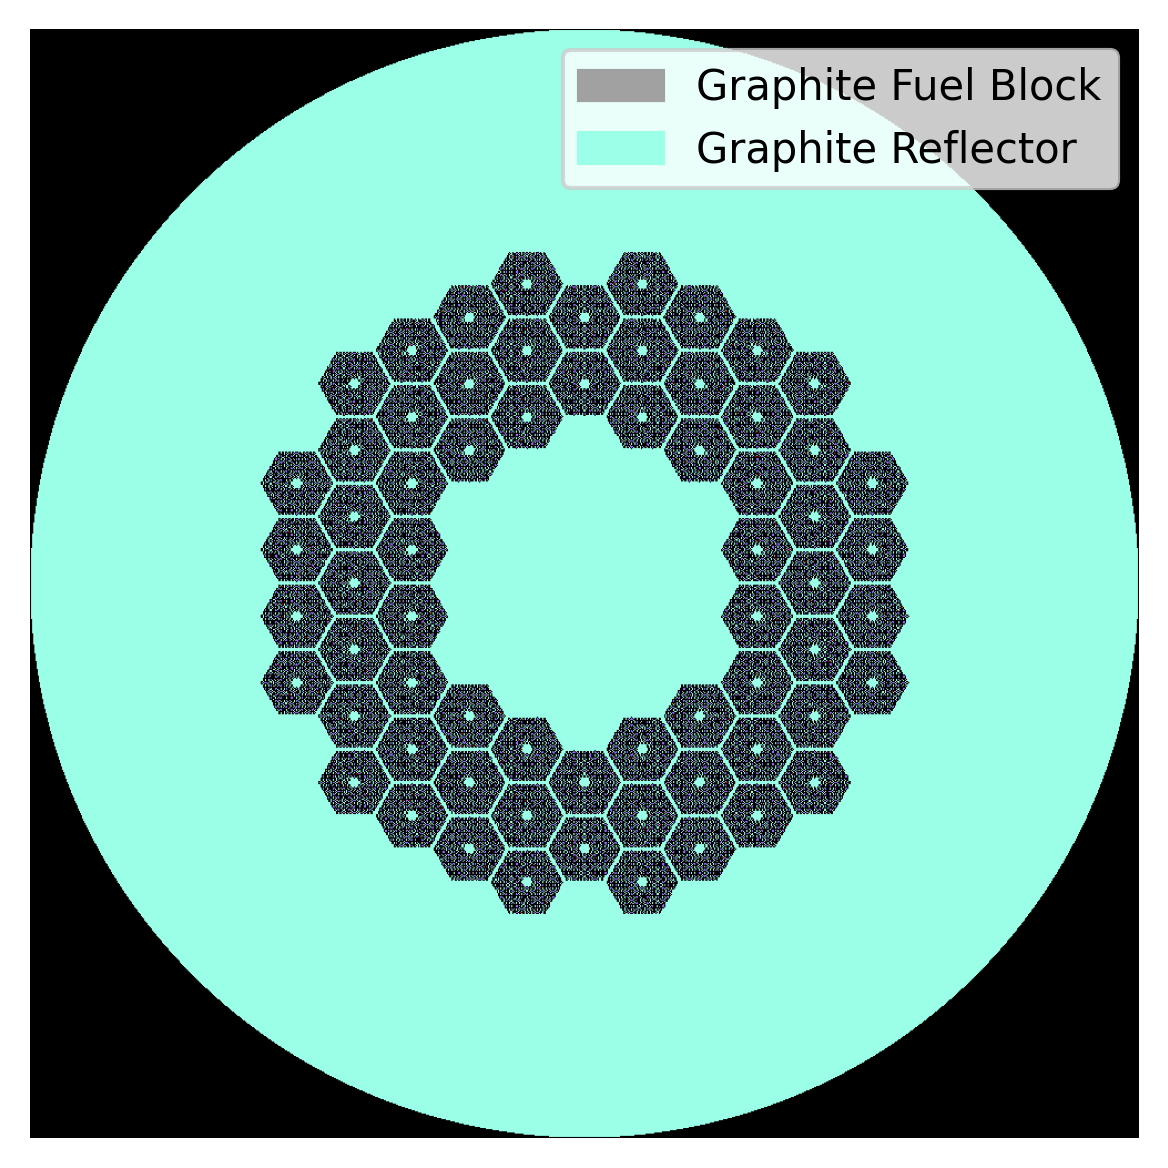
\includegraphics[width=0.39\textwidth]{figures-fullcore/oecd-fullcore}
    }
    \subfloat[Moltres model geometry.]{
        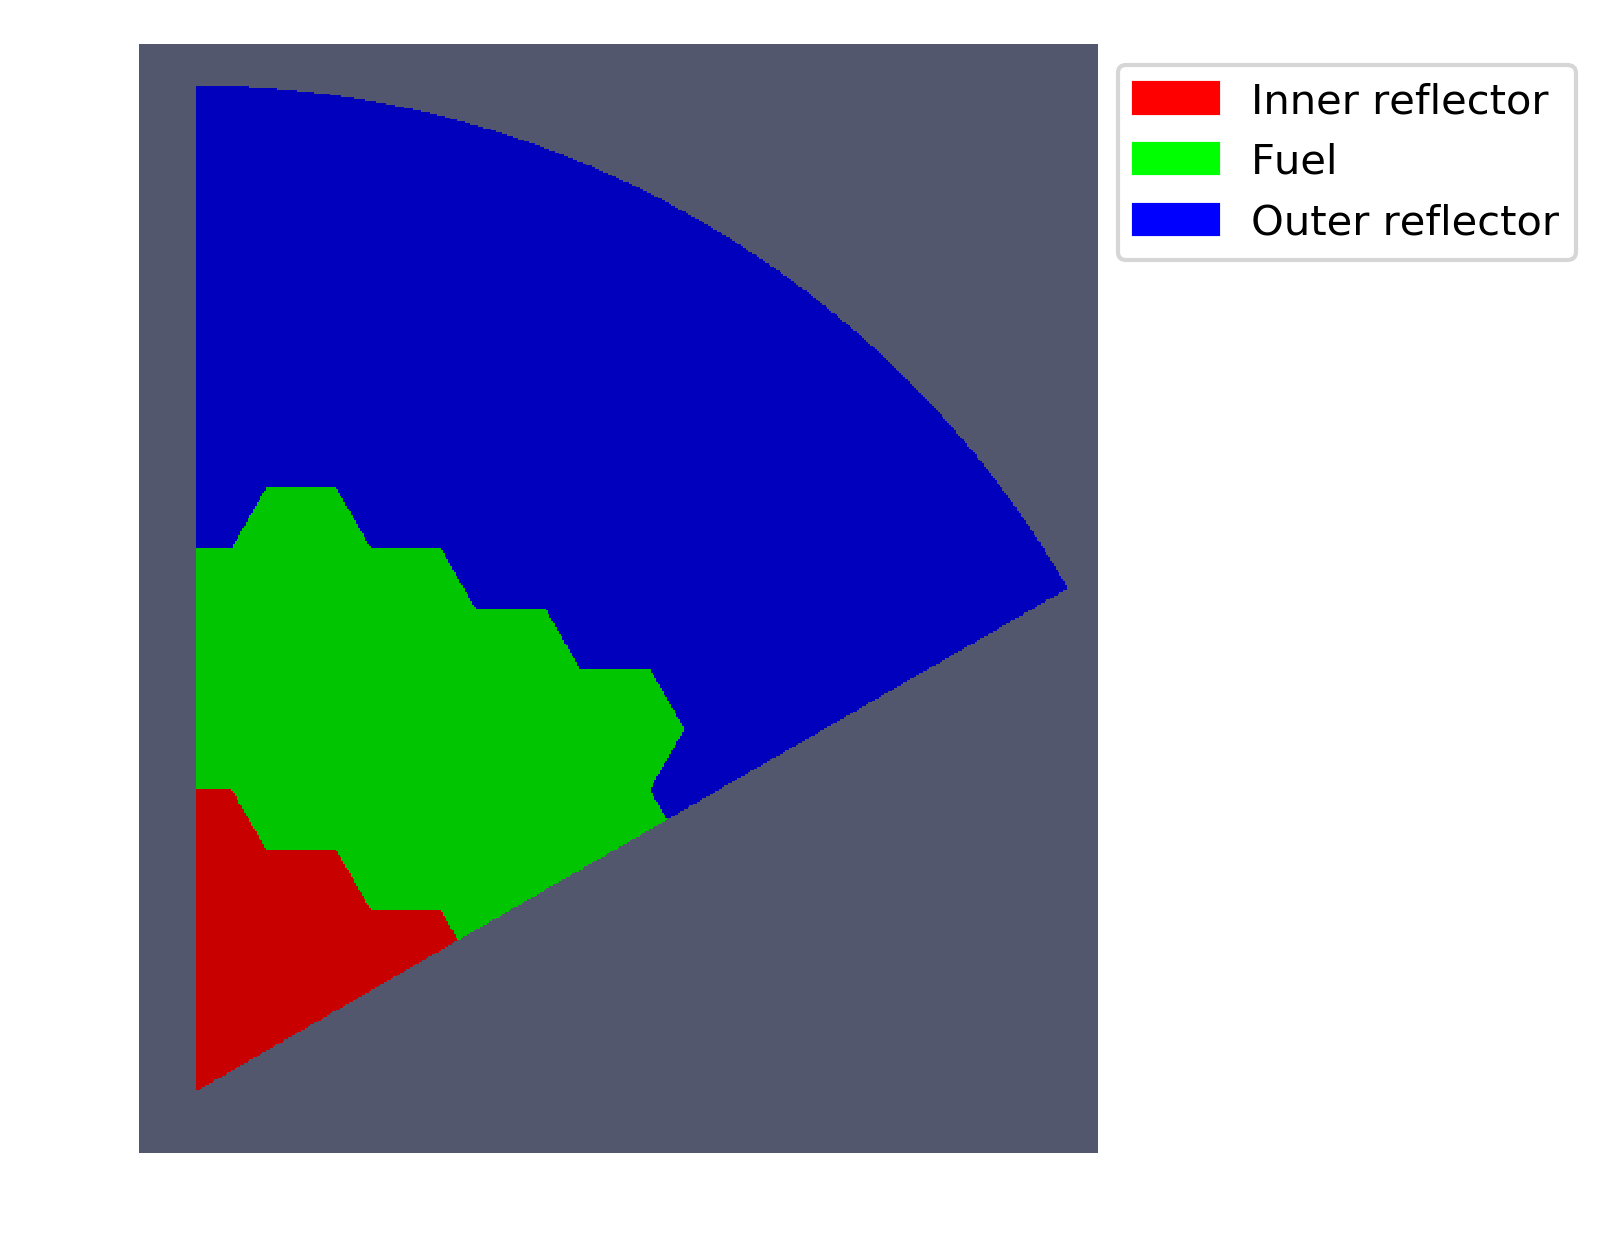
\includegraphics[width=0.49\textwidth]{figures-fullcore/3D-fullcore-60-homo-meshB2}
    }
	\hfill
  \caption{MHTGR-350 full-core models.}
	\label{fig:fullcoremodel}
\end{figure}

\begin{table}[htbp!]
  \centering
  \caption{Serpent and Moltres eigenvalues.}
  \begin{tabular}{l|lll}
  \toprule
              & Serpent			& Moltres  & $\Delta \rho$ [pcm] 	\\
  \midrule
			 600K  	& 1.10869     & 1.11150	 &	228		\\
			1200K 	& 1.06138     & 1.06468	 &	292   \\

  \bottomrule
  \end{tabular}
  \label{tab:full-keff}
\end{table}

%Power distribution at 600K
\begin{figure}[htbp!]
	\centering
    \subfloat[Moltres.]{
        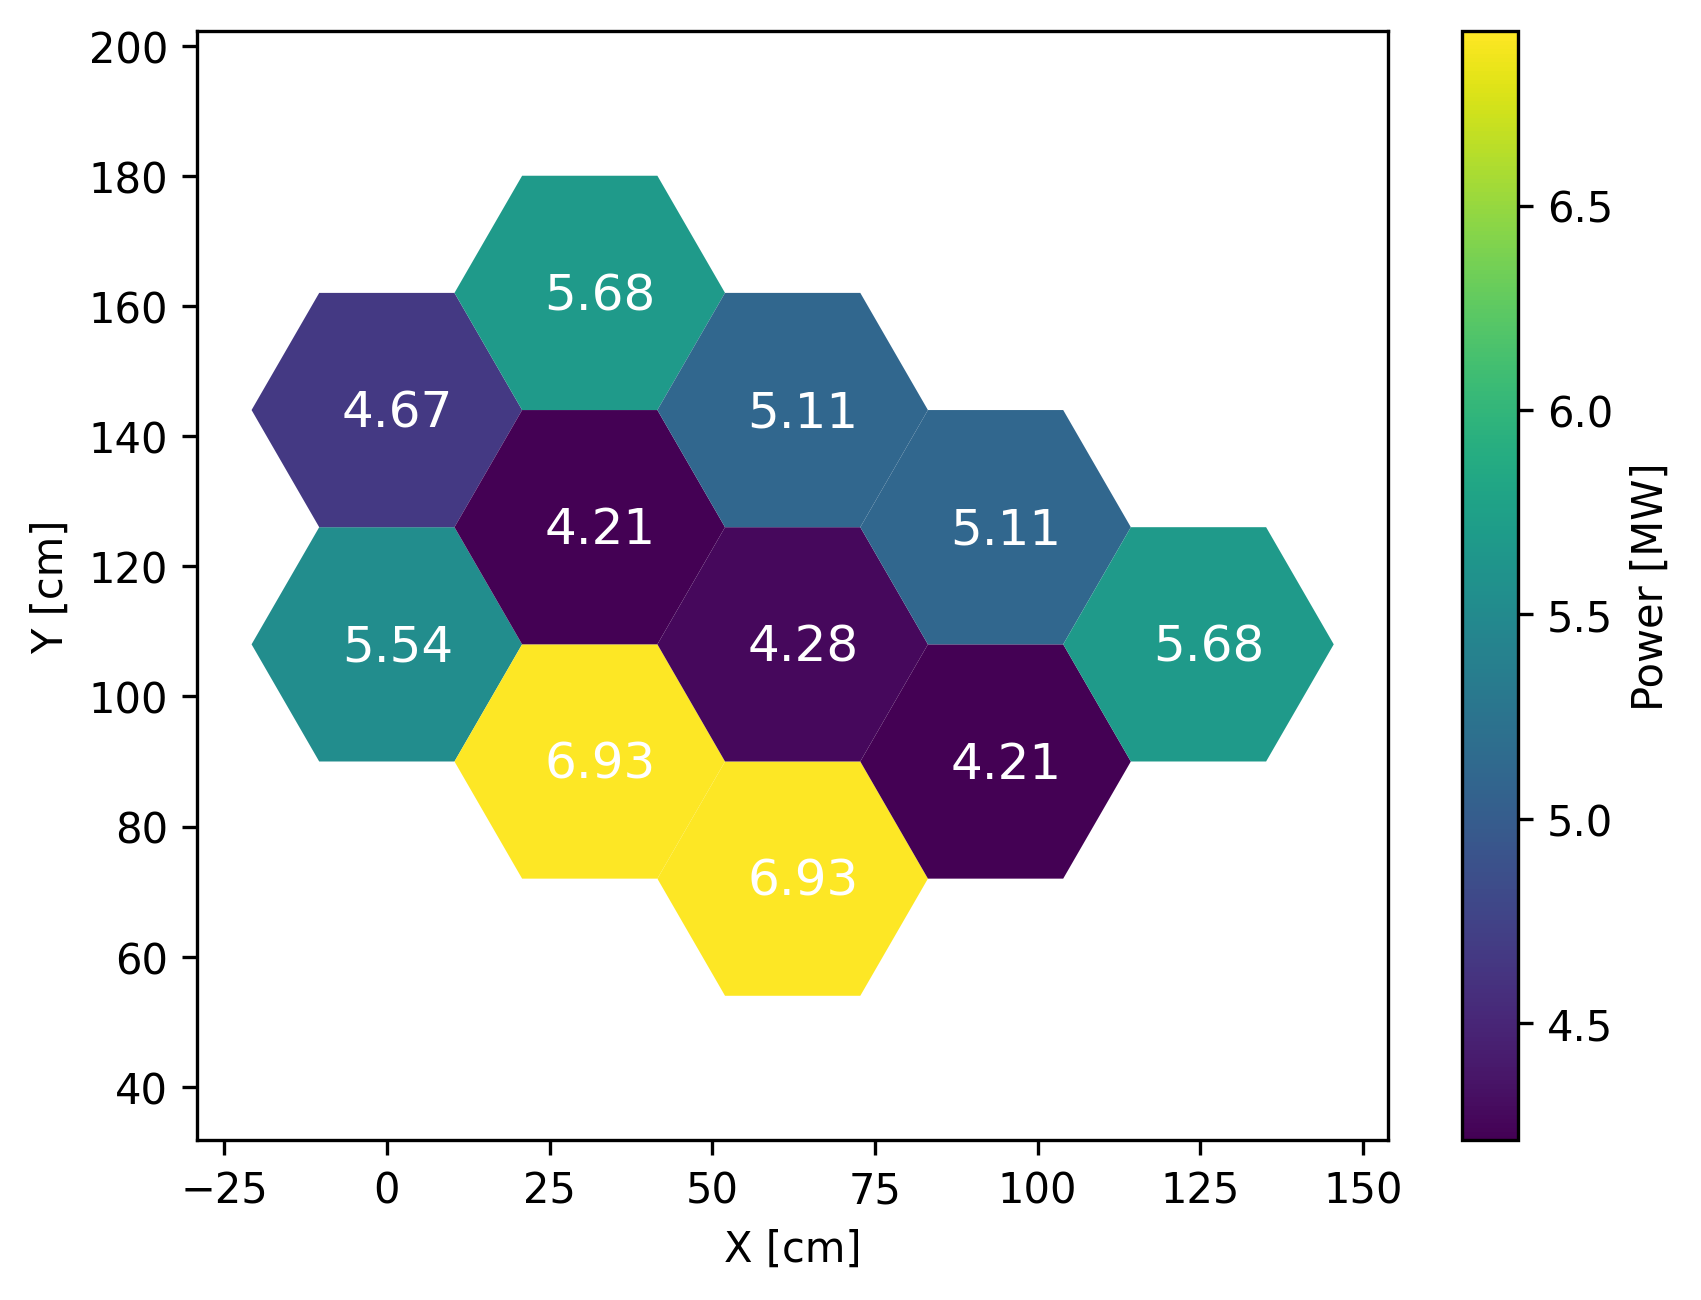
\includegraphics[width=0.45\textwidth]{figures-fullcore/3D-fullcore-600-15Gd-power}
    }
    \subfloat[Serpent.]{
        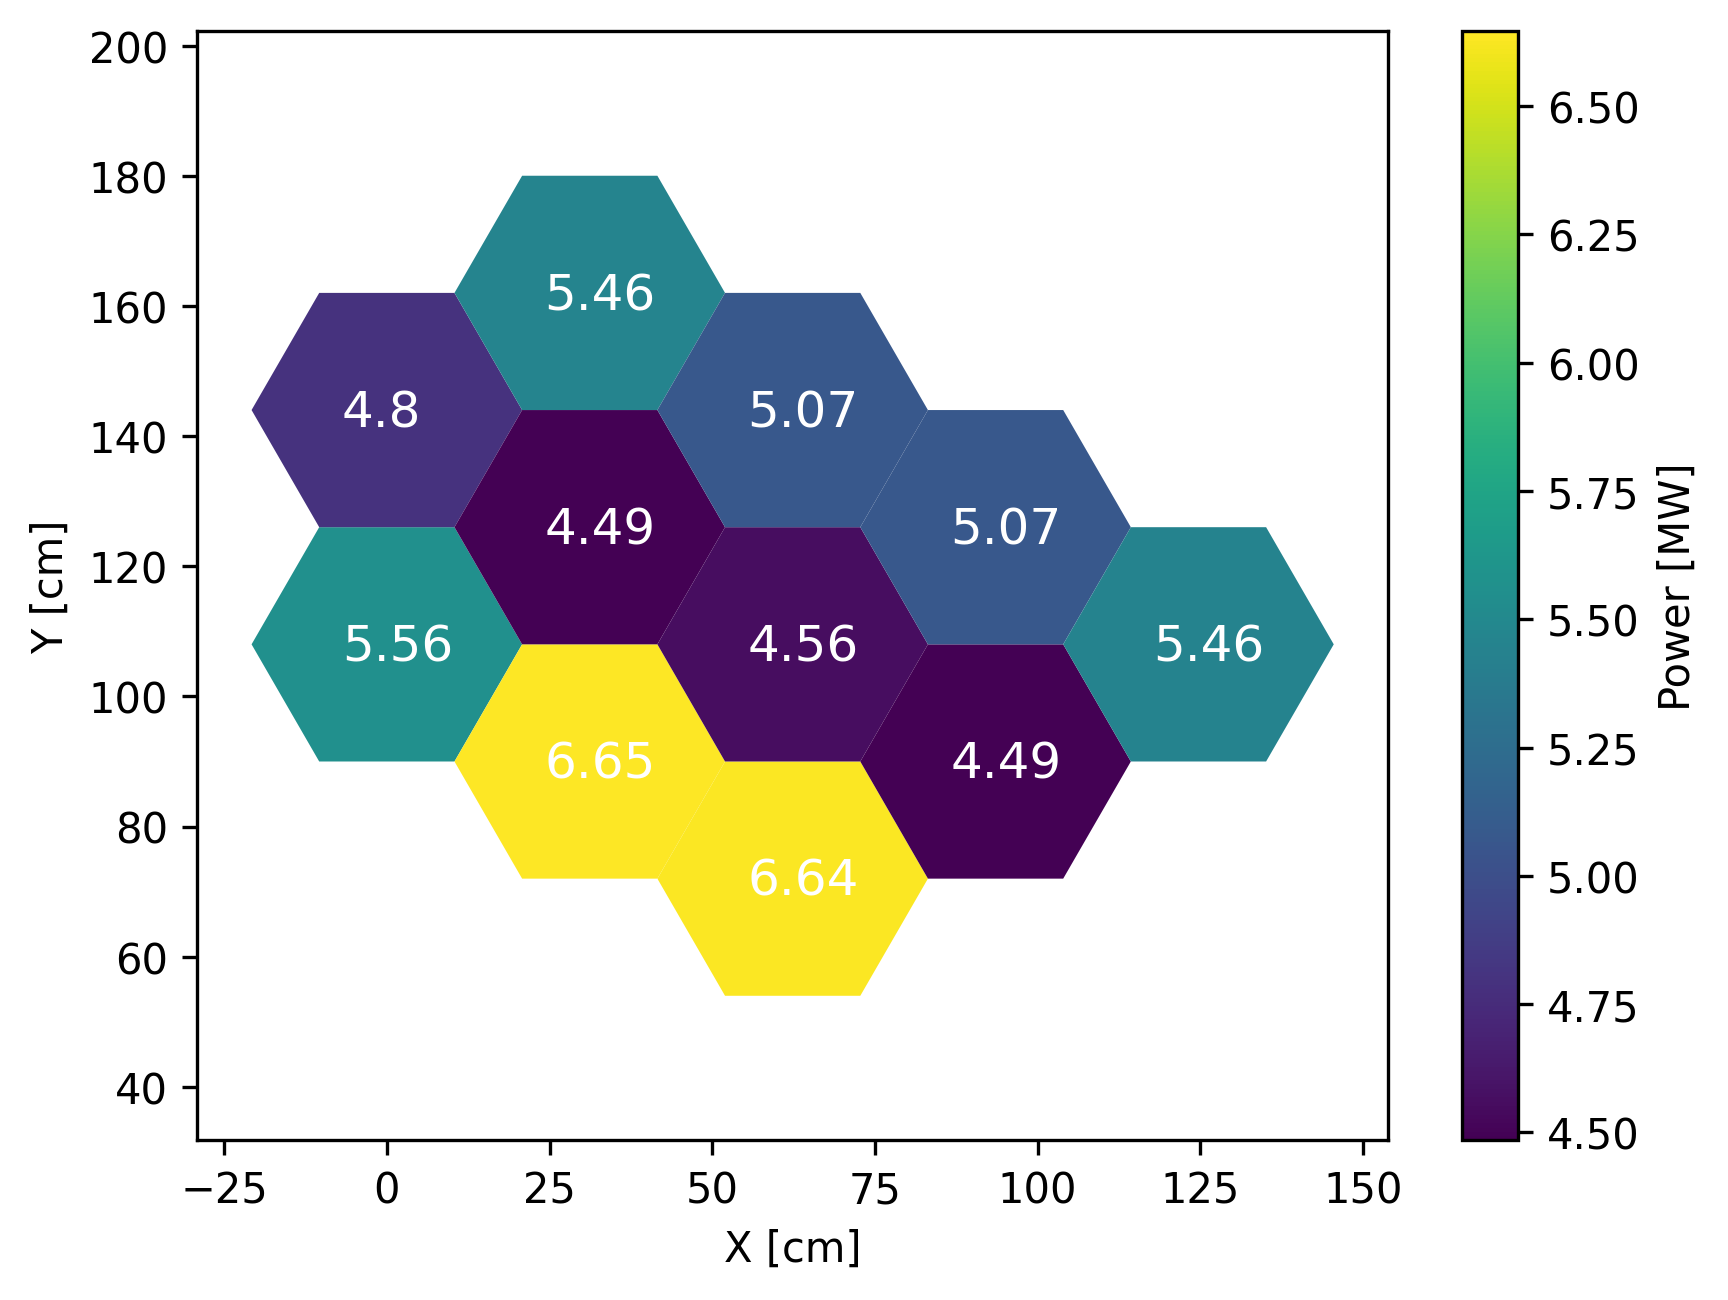
\includegraphics[width=0.45\textwidth]{figures-fullcore/serpent26G-600-power}
    }
	\hfill
	\caption{Radial power distribution at 600 K.}
	\label{fig:fullcore-600-power}
\end{figure}

%Power distribution at 1200K
\begin{figure}[htbp!]
	\centering
    \subfloat[Moltres.]{
        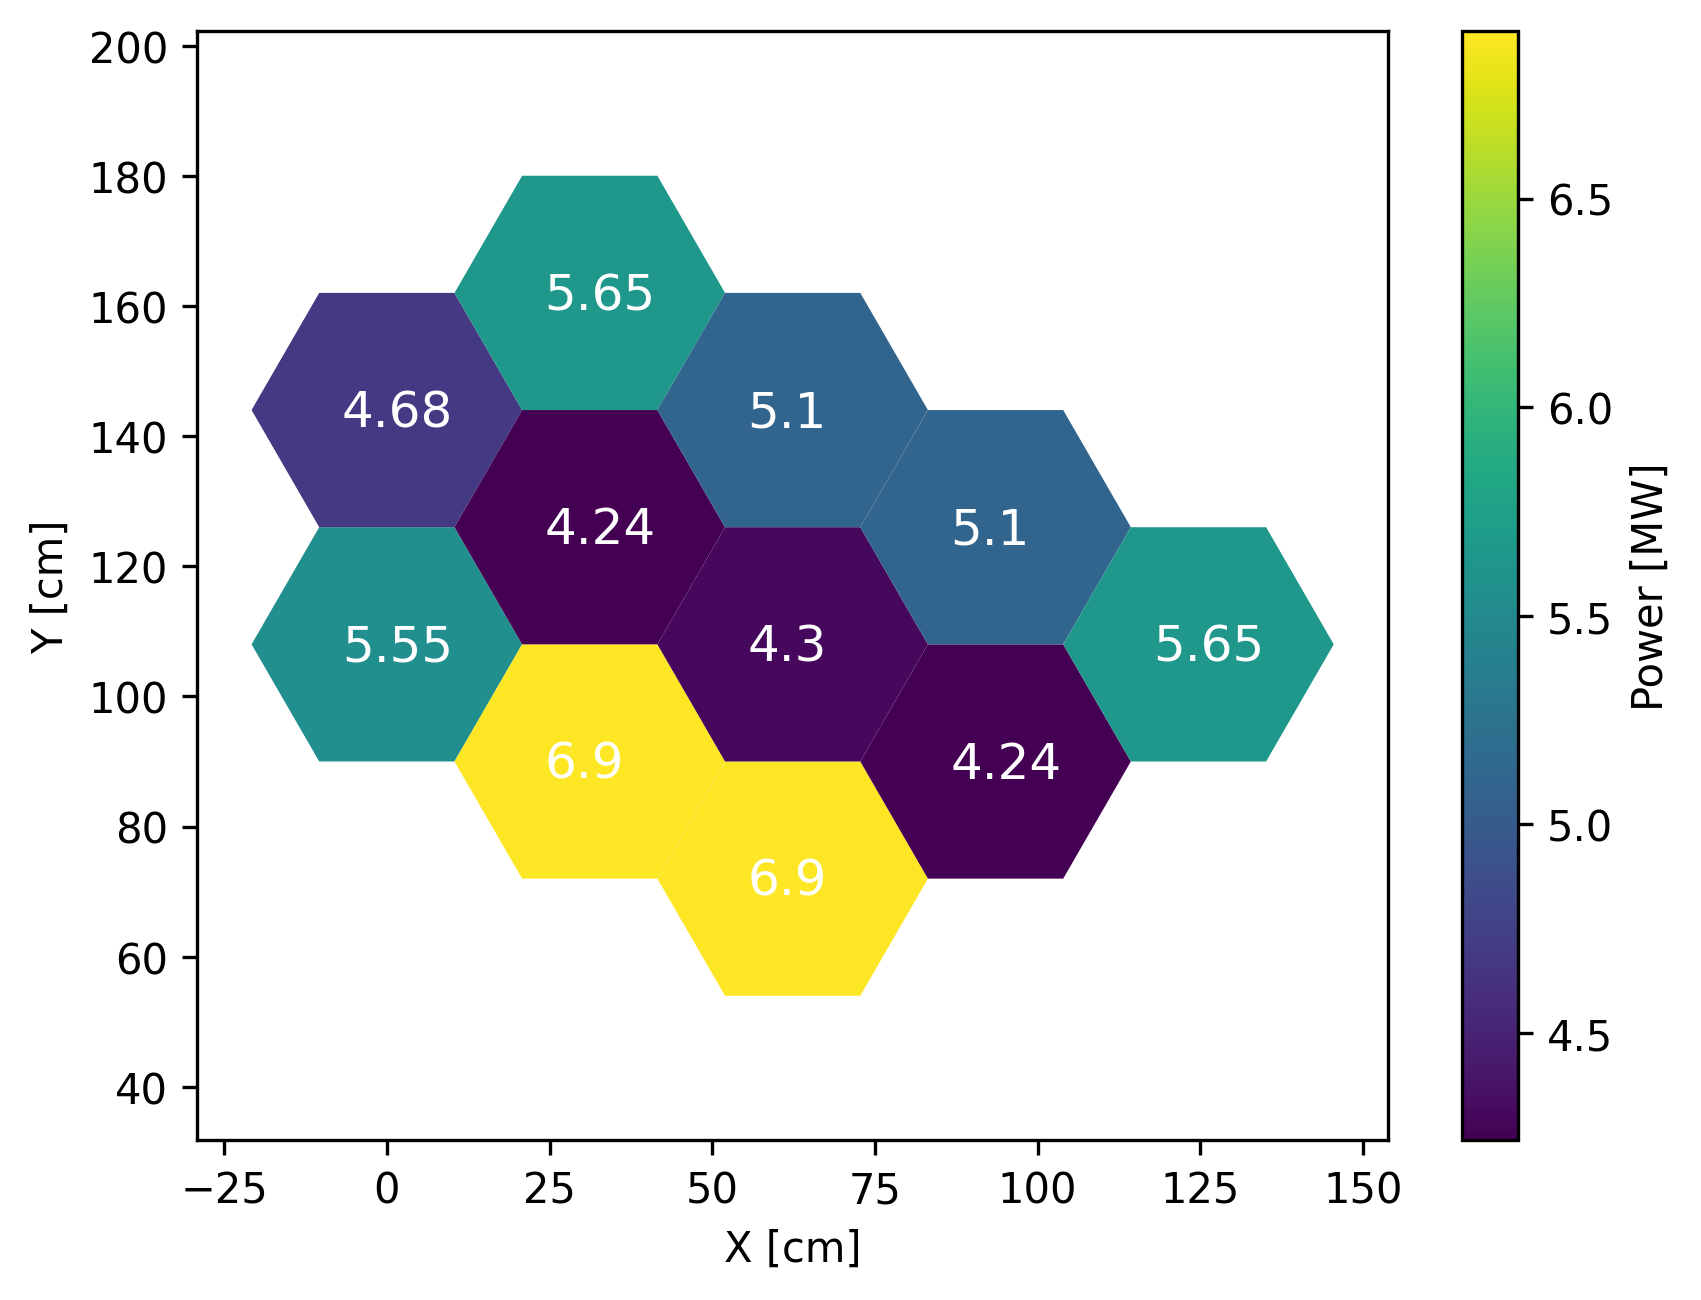
\includegraphics[width=0.45\textwidth]{figures-fullcore/3D-fullcore-1200-15Gc-power}
    }
    \subfloat[Serpent.]{
        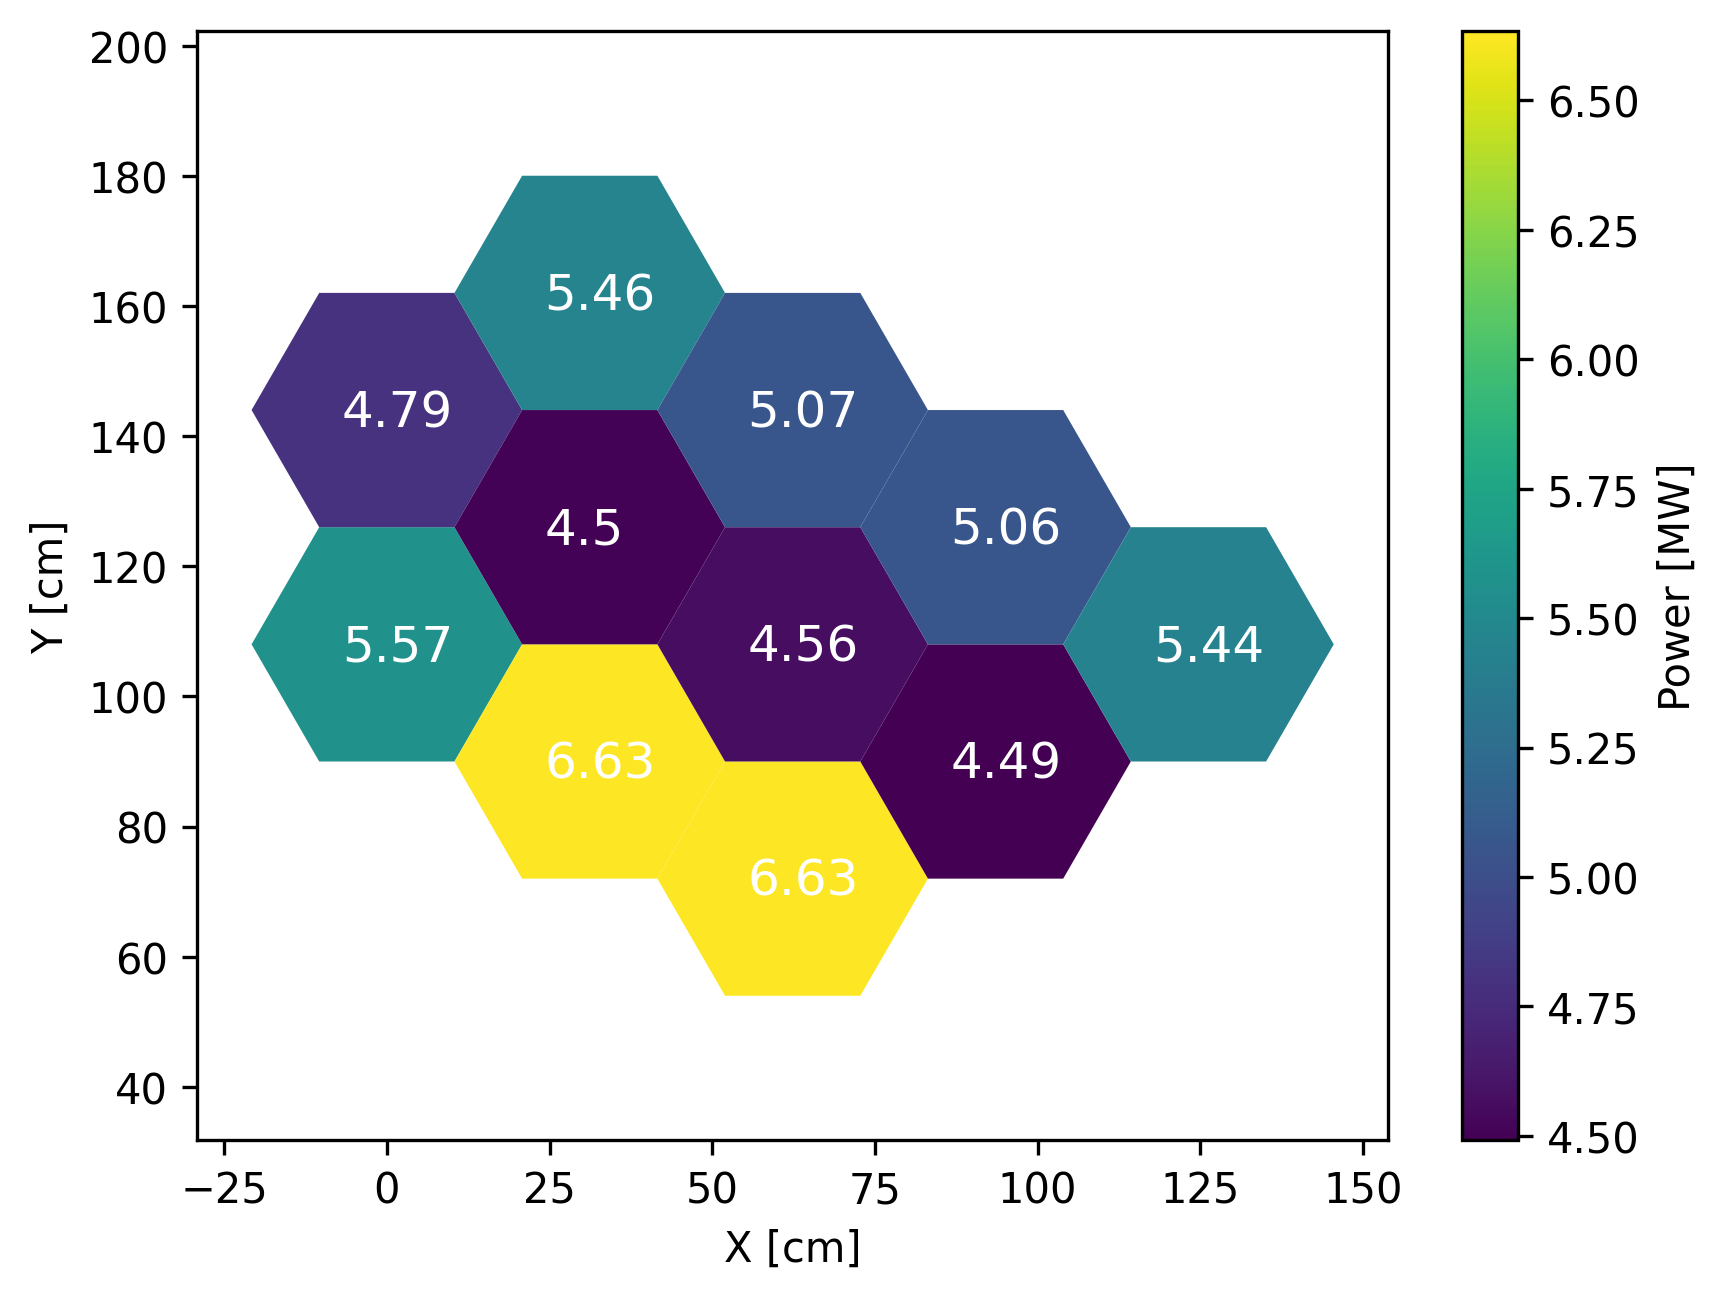
\includegraphics[width=0.45\textwidth]{figures-fullcore/serpent26G-1200-power}
    }
	\hfill
	\caption{Radial power distribution at 1200 K.}
	\label{fig:fullcore-1200-power}
\end{figure}

%Detectors
\begin{figure}[htbp!]
	\centering
    \subfloat[]{
        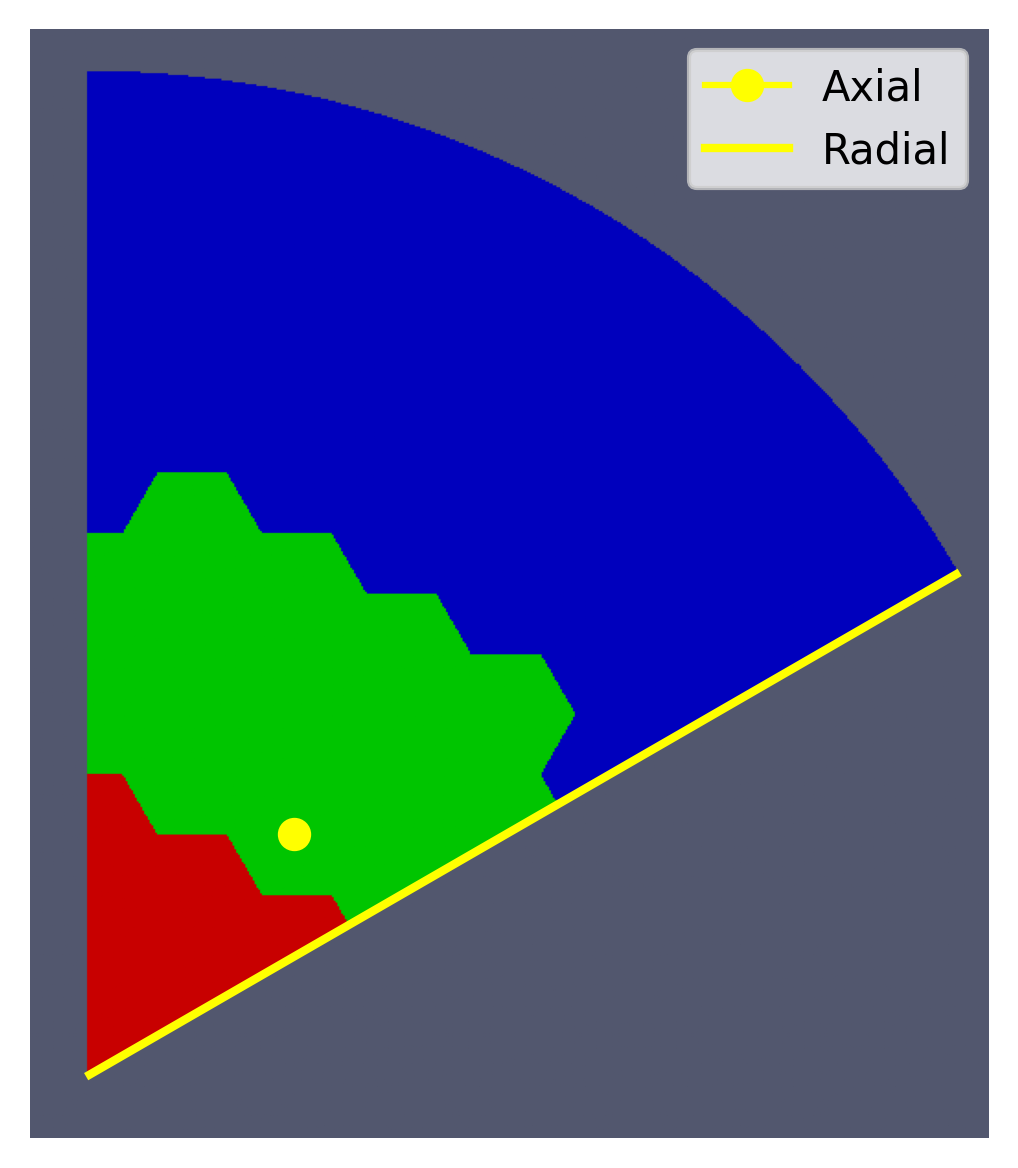
\includegraphics[width=0.37\textwidth]{figures-fullcore/3D-fullcore-60-detectors2}
    }
    \subfloat[Serpent model geometry.]{
        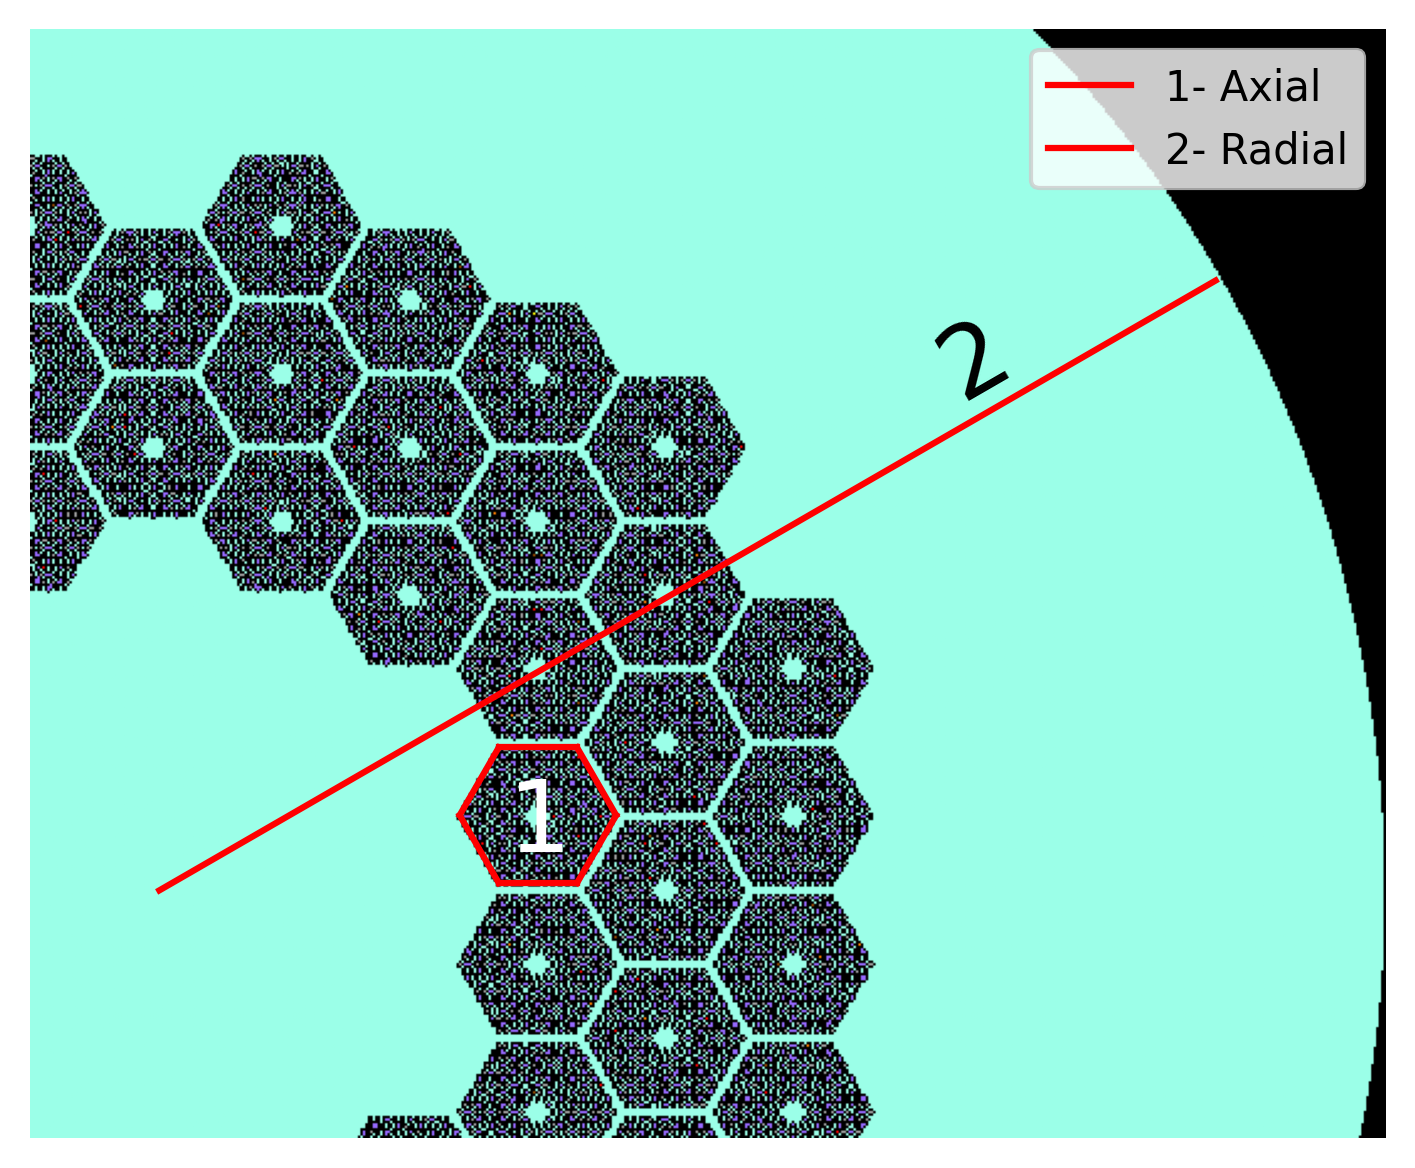
\includegraphics[width=0.52\textwidth]{figures-fullcore/oecd-fullcore-detectorsC}
    }
	\hfill
	\caption{Flux detector locations.}
	\label{fig:fullcore-detectors}
\end{figure}

% Axial flux1 at 600K
\begin{figure}[htbp!]
	\centering
    \subfloat[]{
        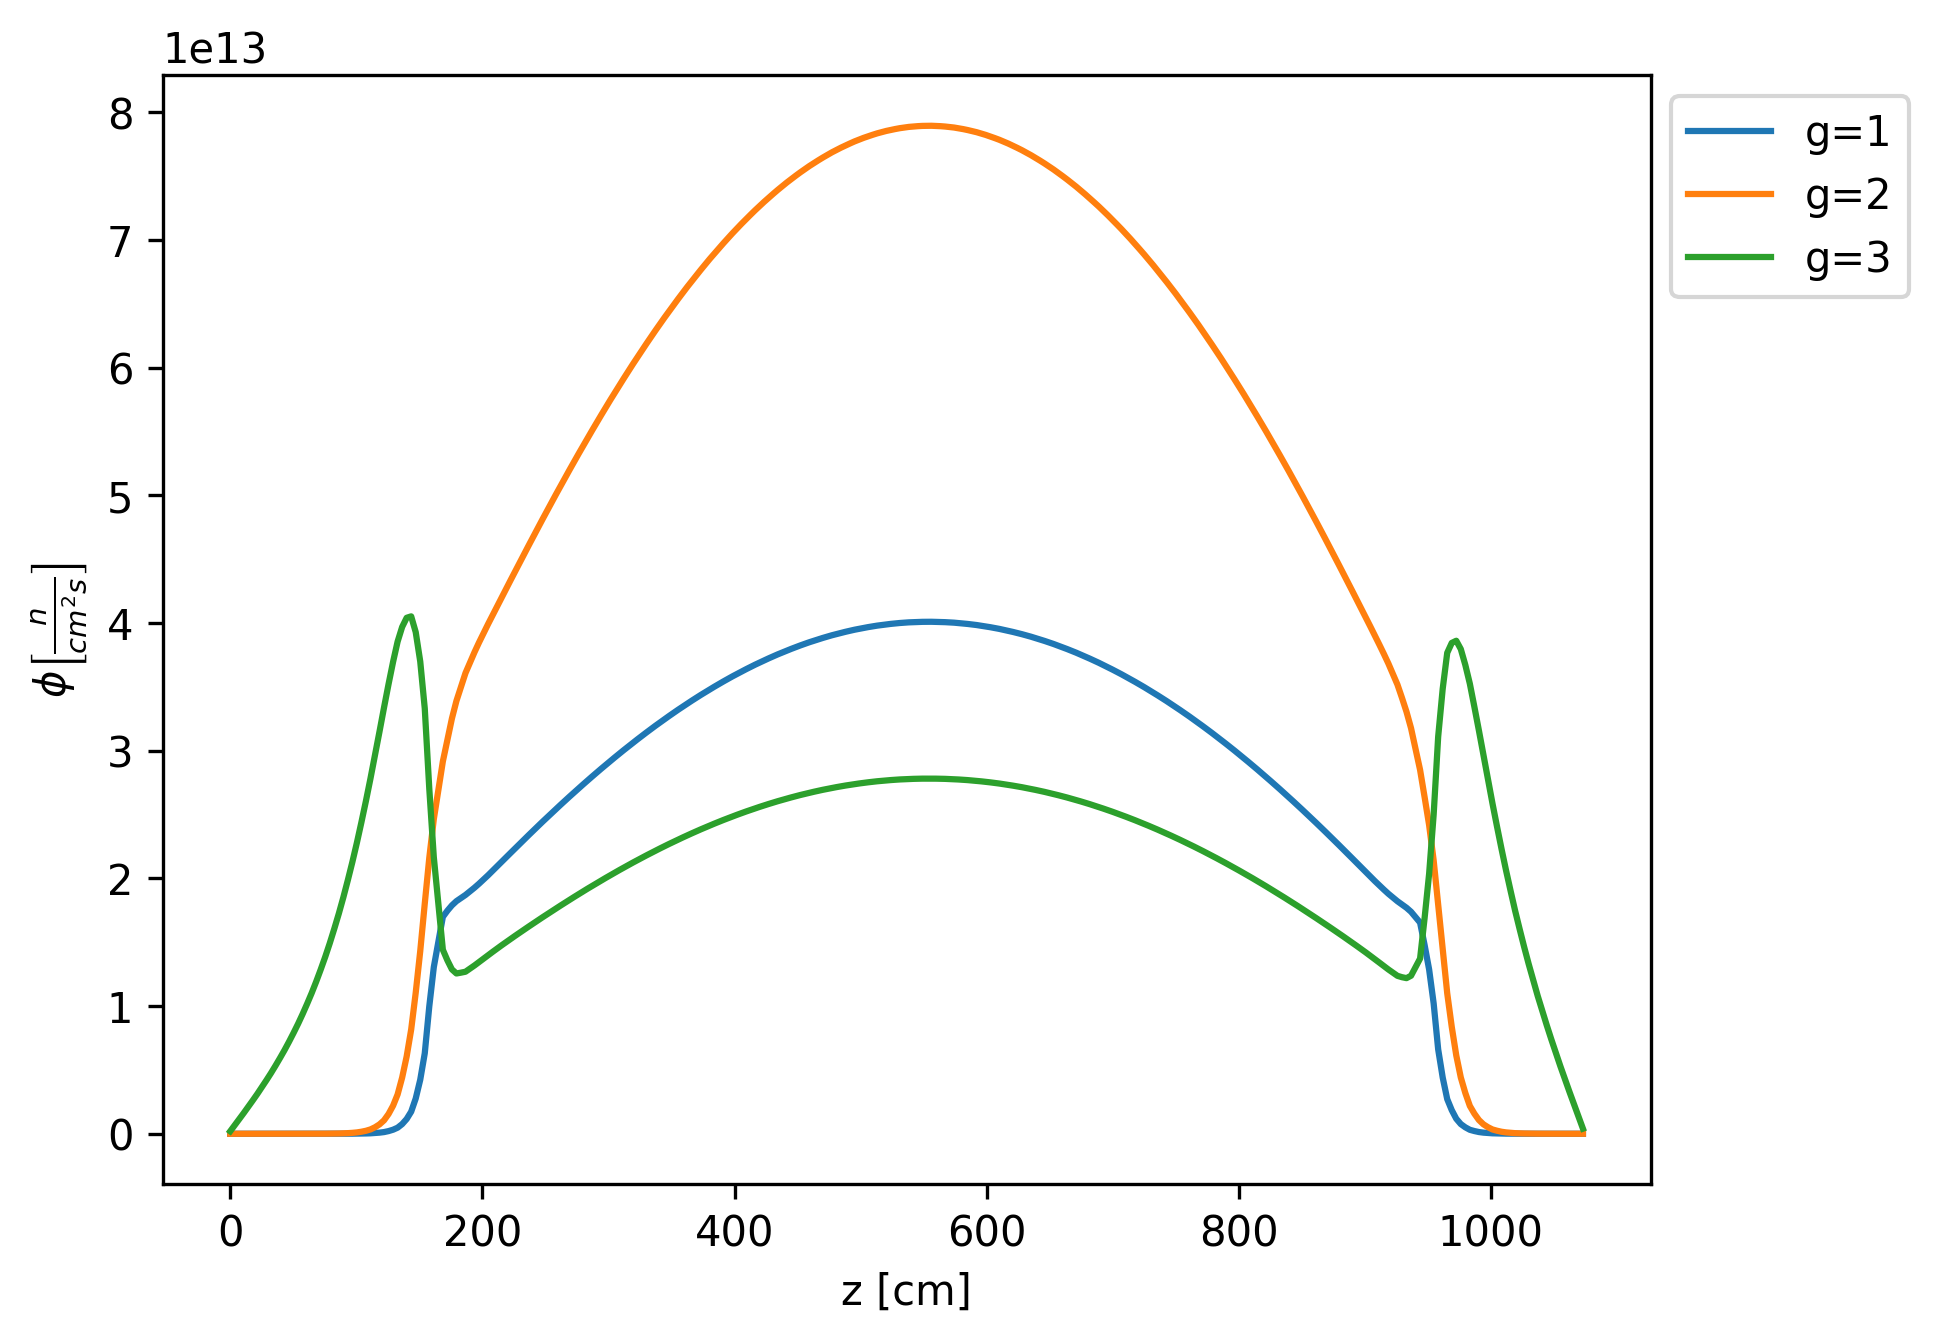
\includegraphics[width=0.45\textwidth]{figures-fullcore/3D-fullcore-600-15Gd-axial1}
    }
    \subfloat[Serpent model geometry.]{
        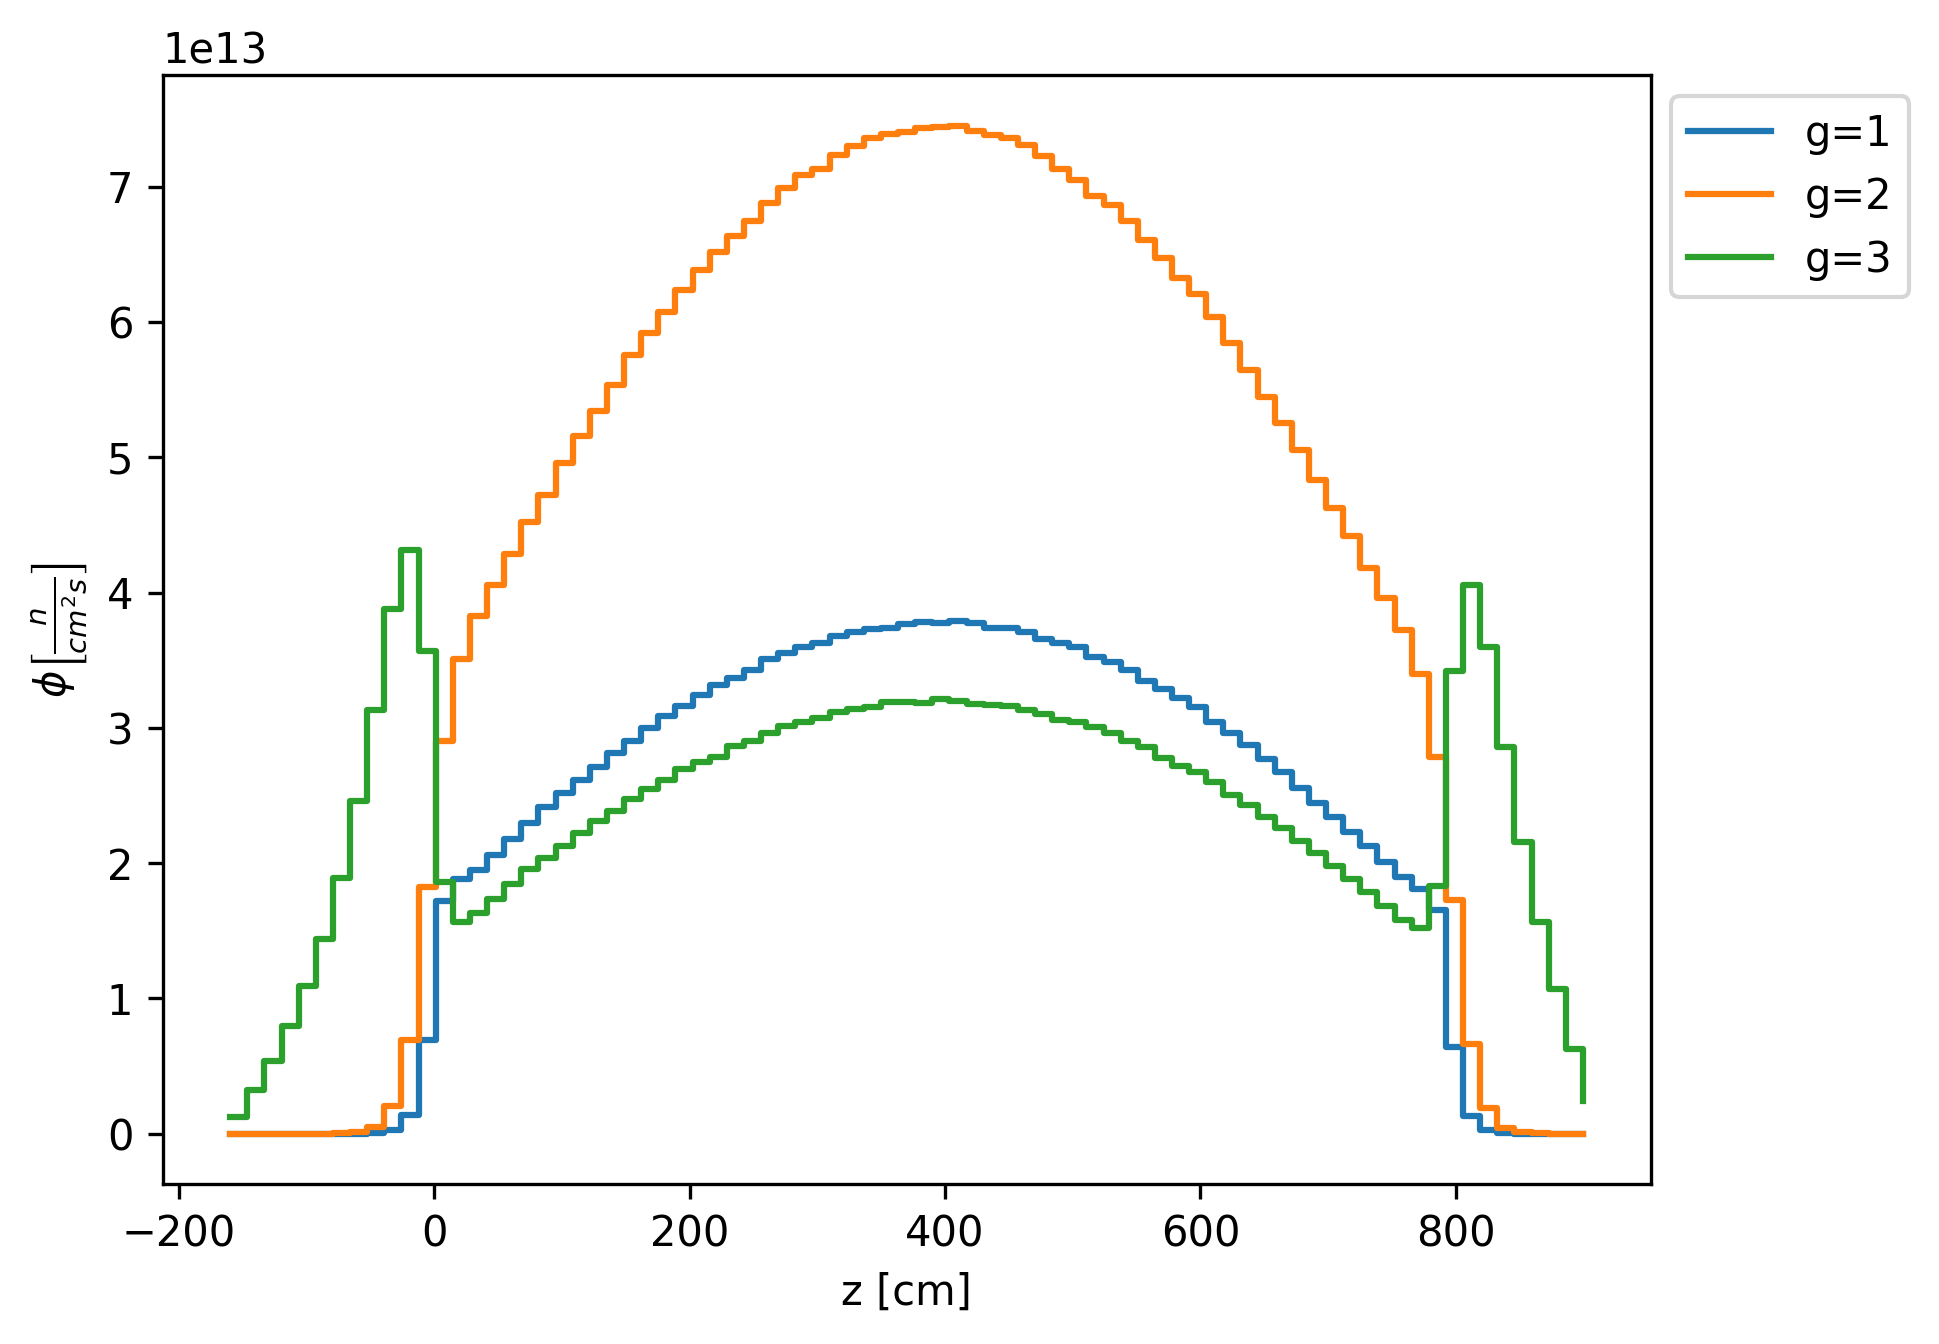
\includegraphics[width=0.45\textwidth]{figures-fullcore/serpent26G-600-collapse-Axial1}
    }
	\hfill
	\caption{Axial flux at 600 K.}
	\label{fig:fullcore-600-axial1}
\end{figure}

%Radial flux at 600 K
\begin{figure}[htbp!]
	\centering
    \subfloat[Moltres.]{
        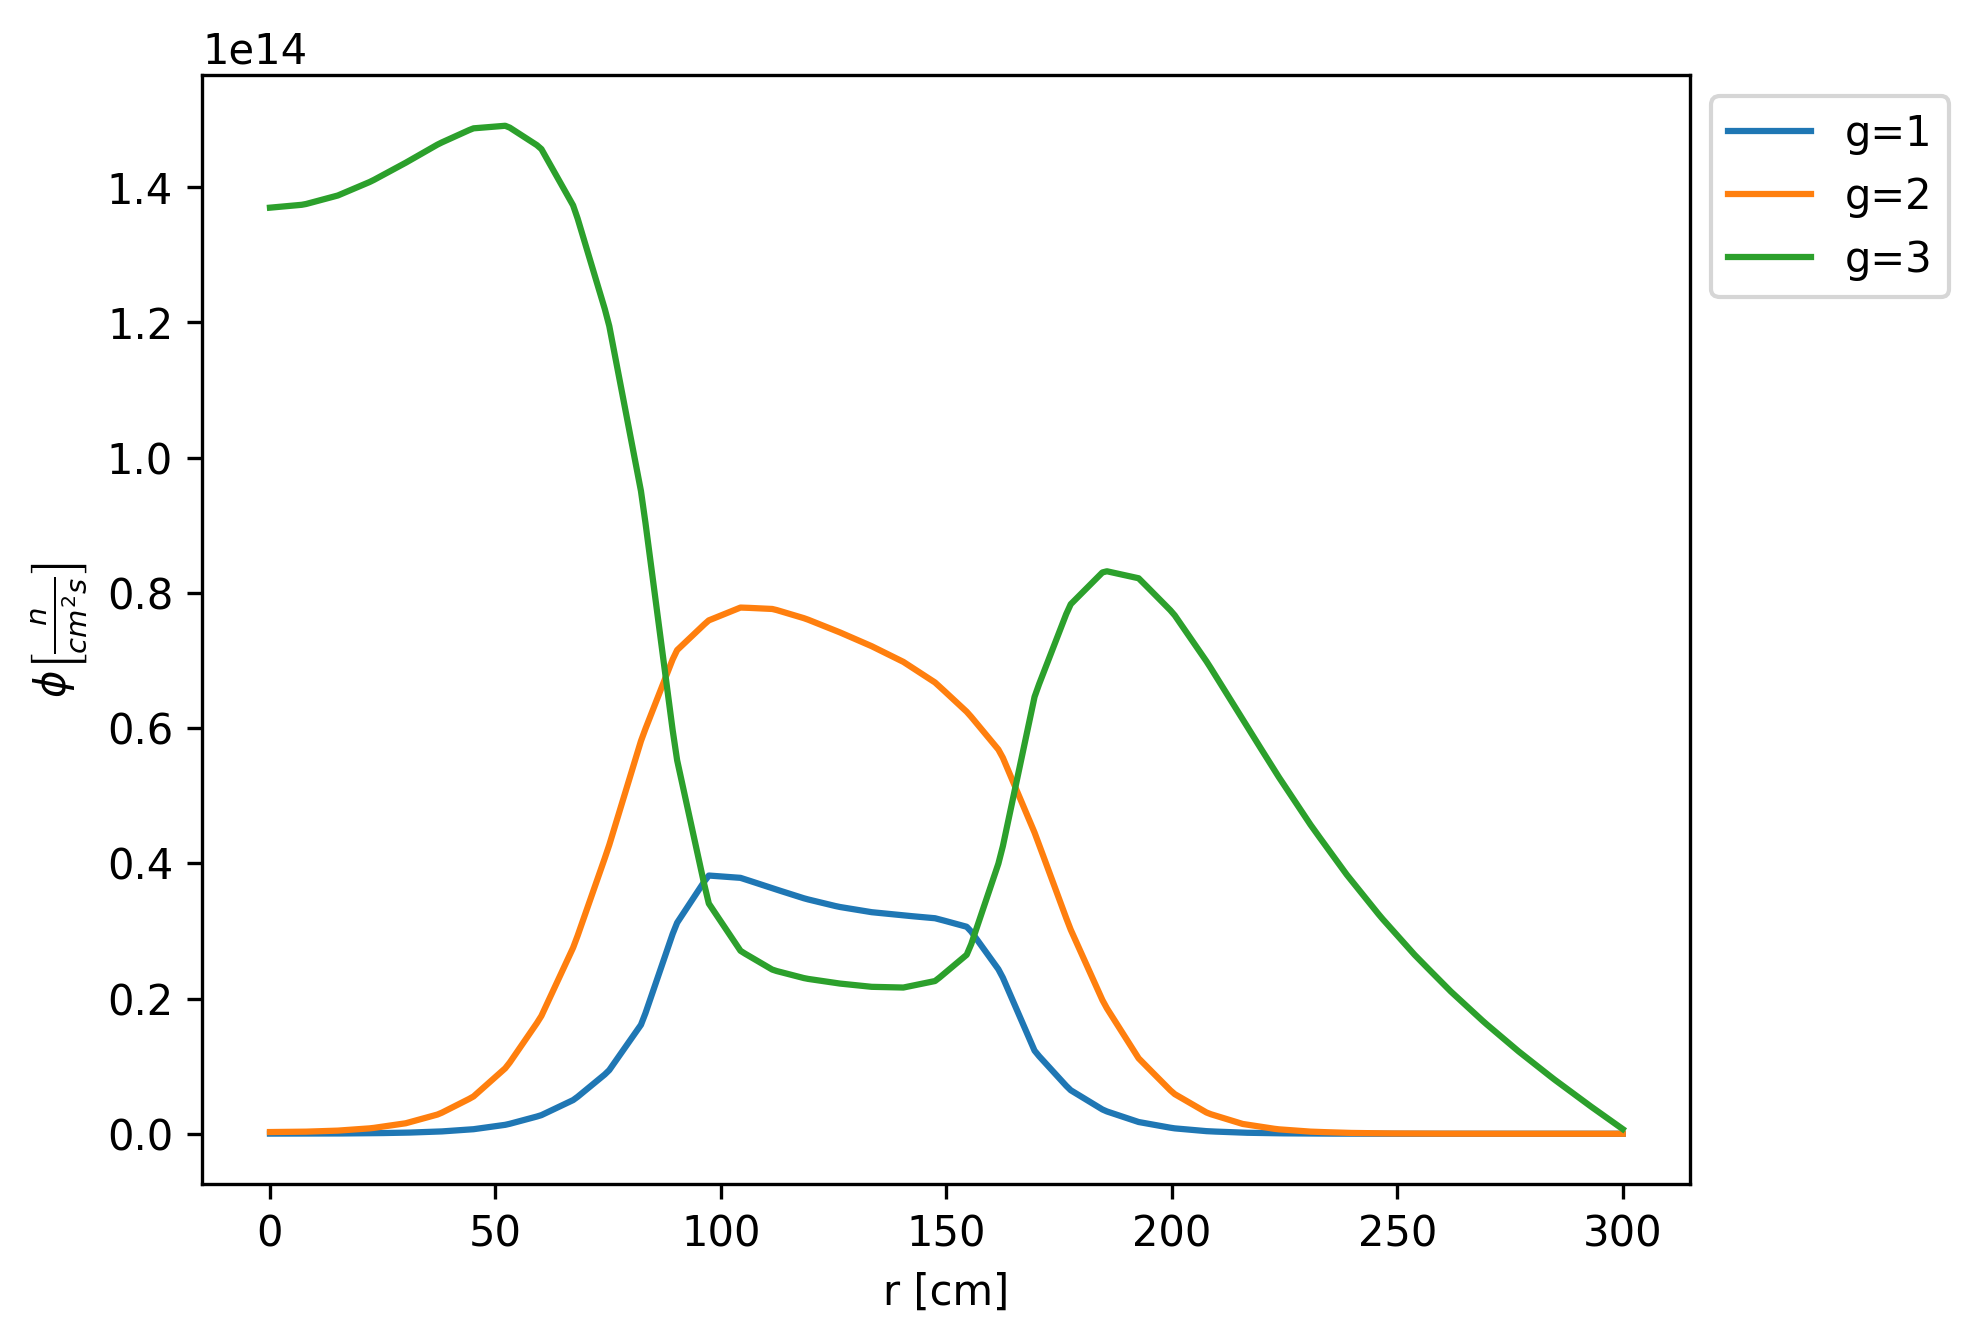
\includegraphics[width=0.45\textwidth]{figures-fullcore/3D-fullcore-600-15Gd-radial1}
    }
    \subfloat[Serpent.]{
        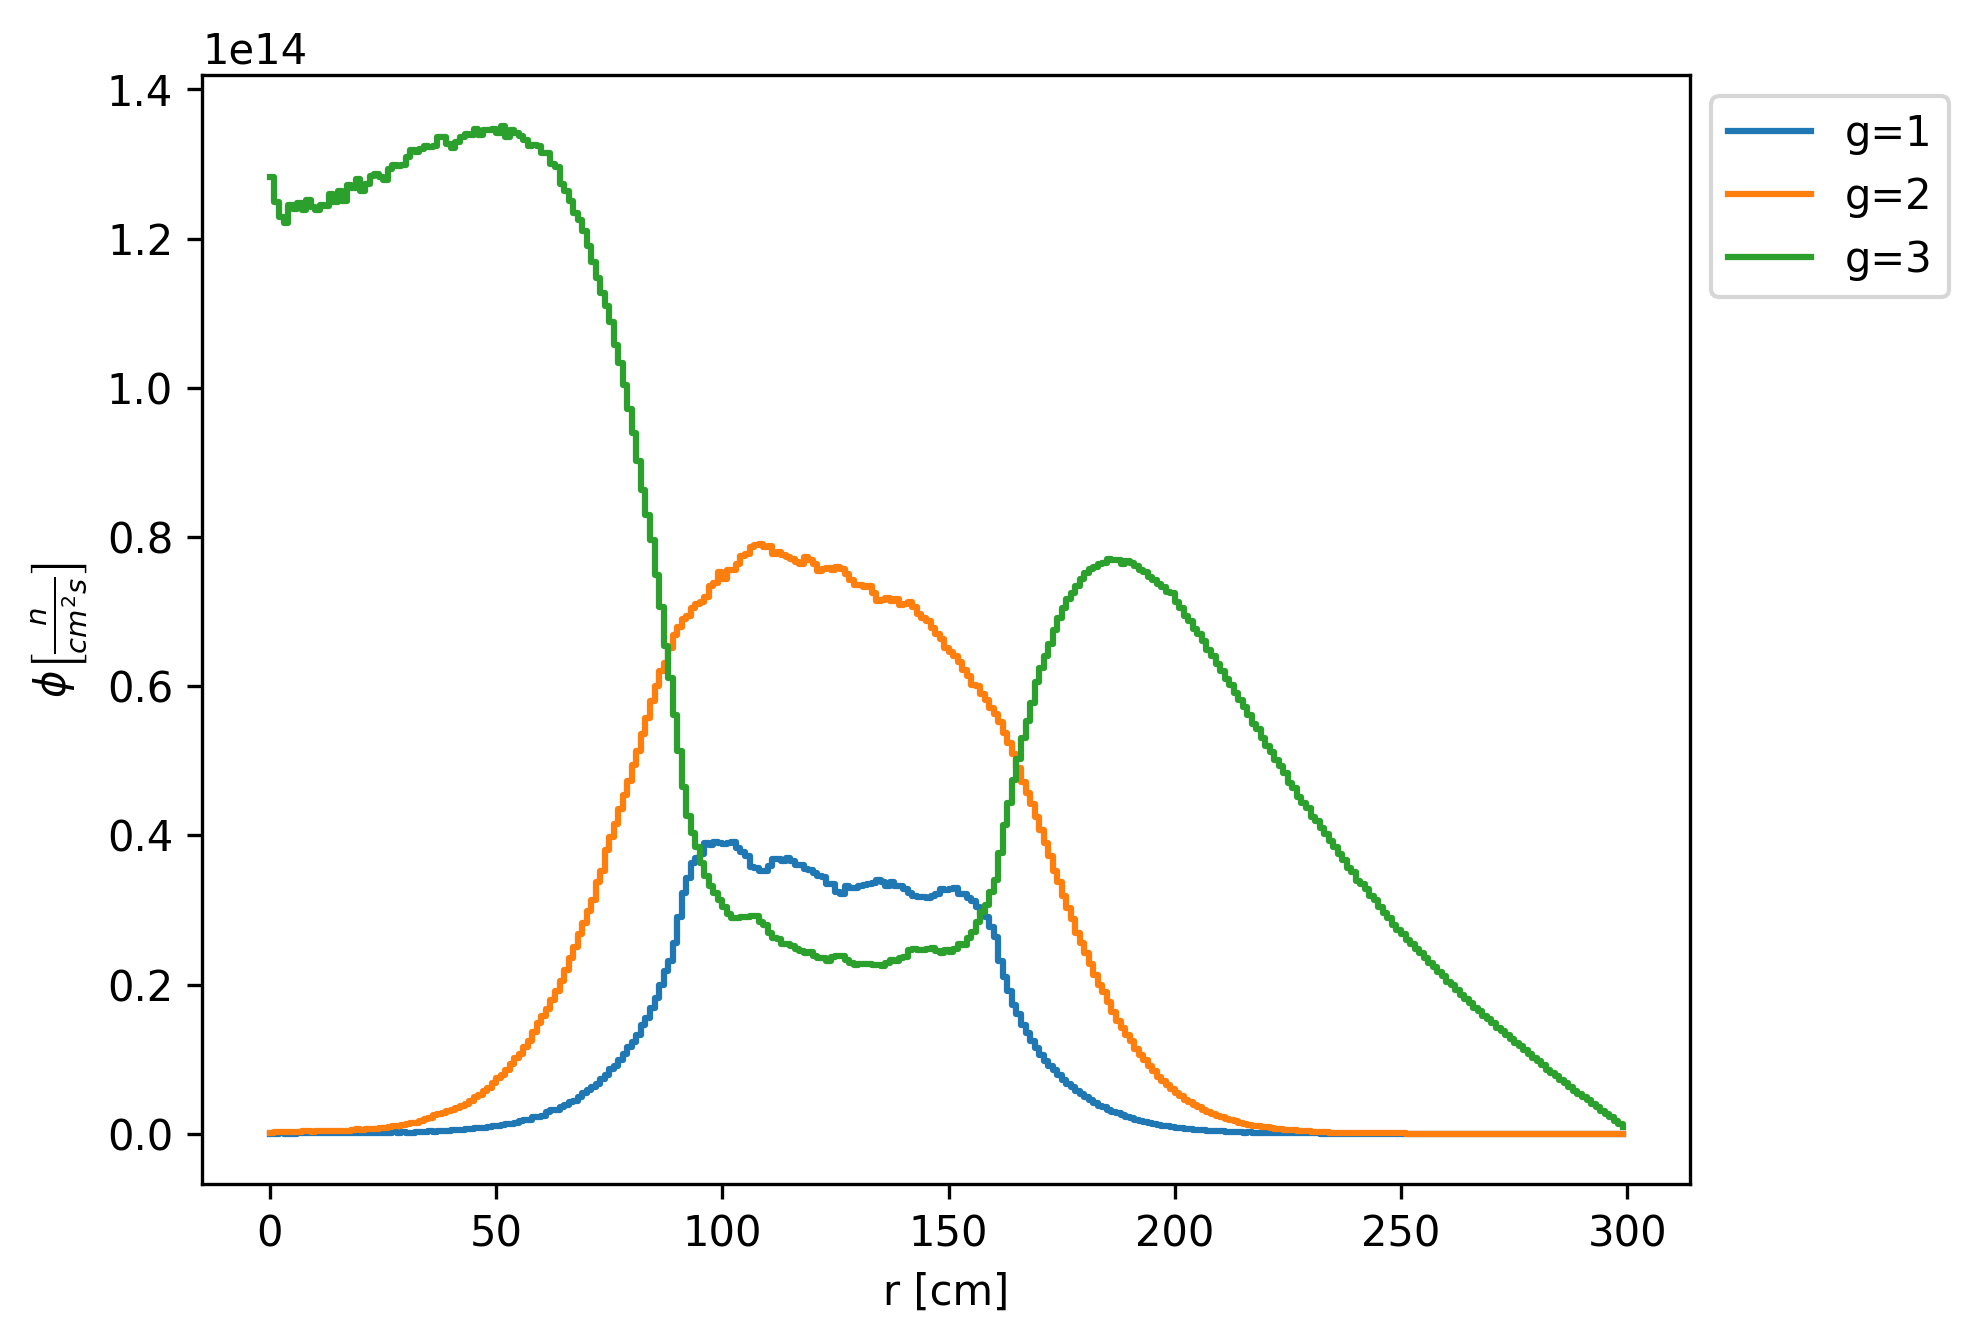
\includegraphics[width=0.45\textwidth]{figures-fullcore/serpent26G-600-collapse-Radial}
    }
	\hfill
	\caption{Radial flux at 600 K.}
	\label{fig:fullcore-600-radial1}
\end{figure}

% Axial flux1 at 1200K
\begin{figure}[htbp!]
	\centering
    \subfloat[]{
        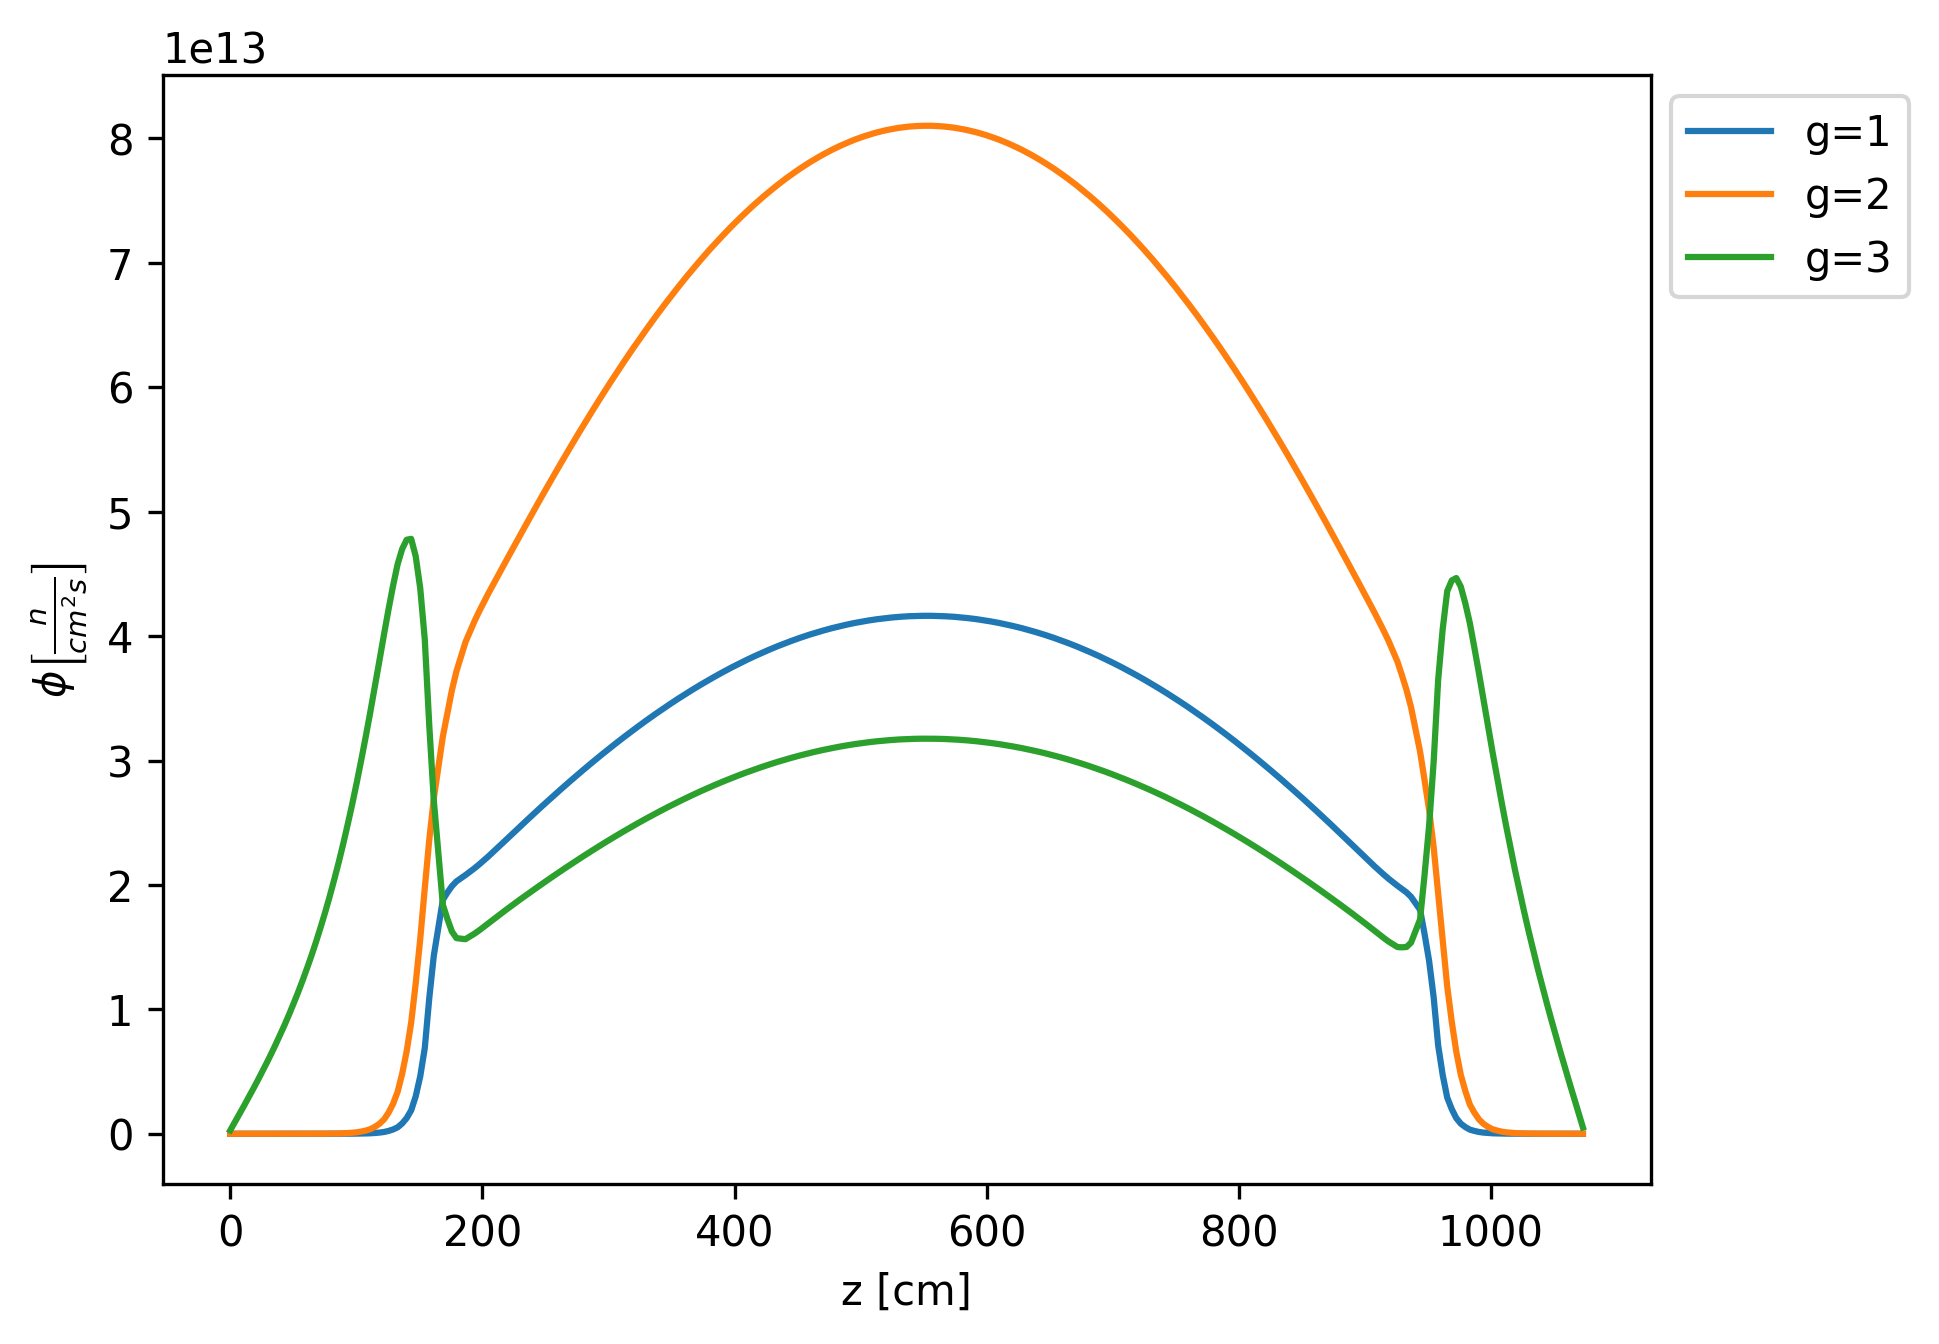
\includegraphics[width=0.45\textwidth]{figures-fullcore/3D-fullcore-1200-15Gc-axial1}
    }
    \subfloat[Serpent model geometry.]{
        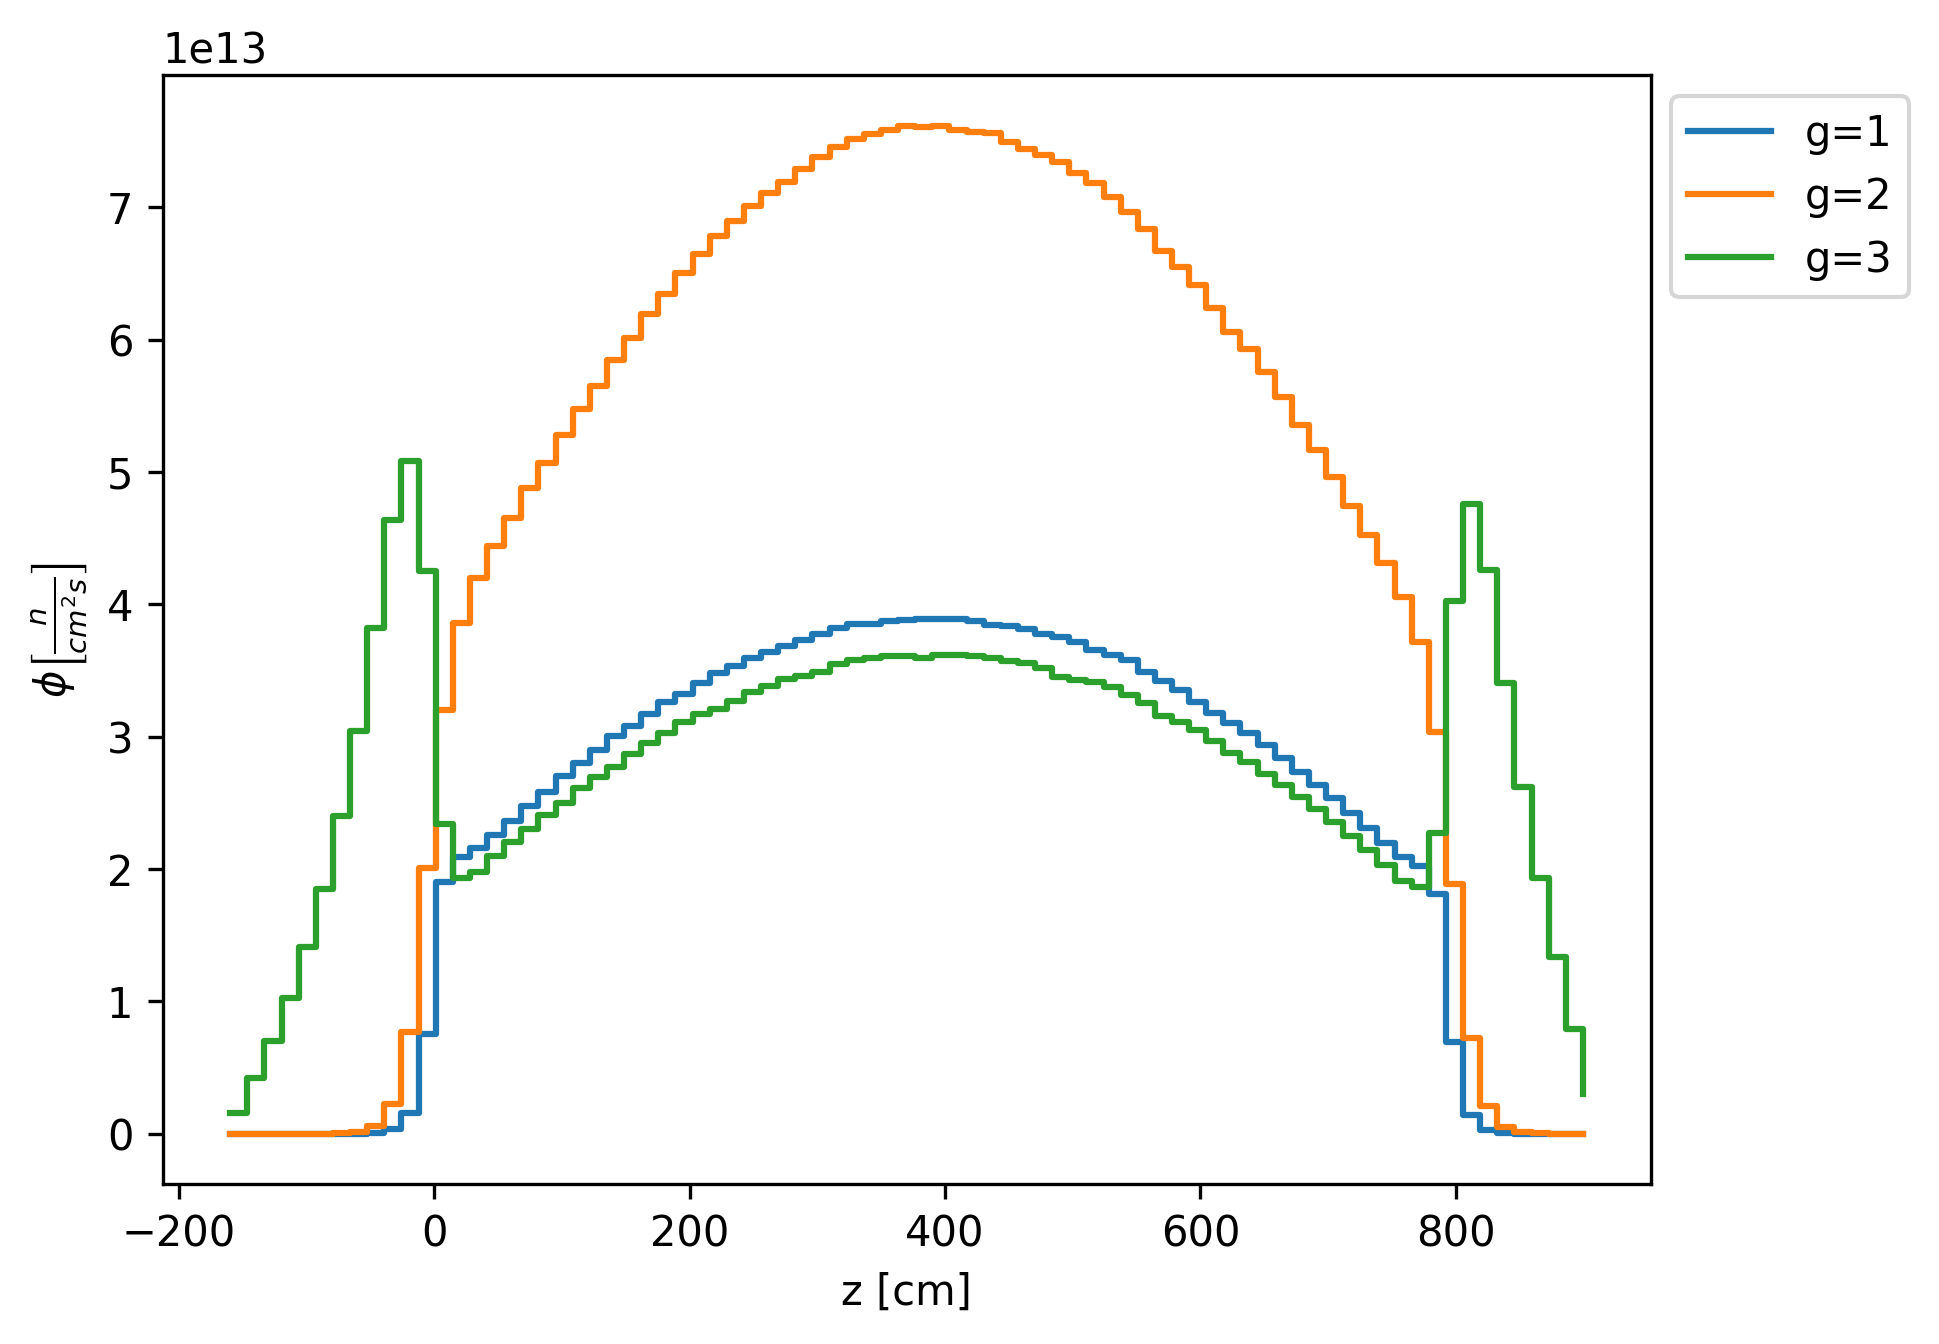
\includegraphics[width=0.45\textwidth]{figures-fullcore/serpent26G-1200-collapse-Axial1}
    }
	\hfill
	\caption{Axial flux at 1200 K.}
	\label{fig:fullcore-1200-axial1}
\end{figure}

%Radial flux at 1200 K
\begin{figure}[htbp!]
	\centering
    \subfloat[Moltres.]{
        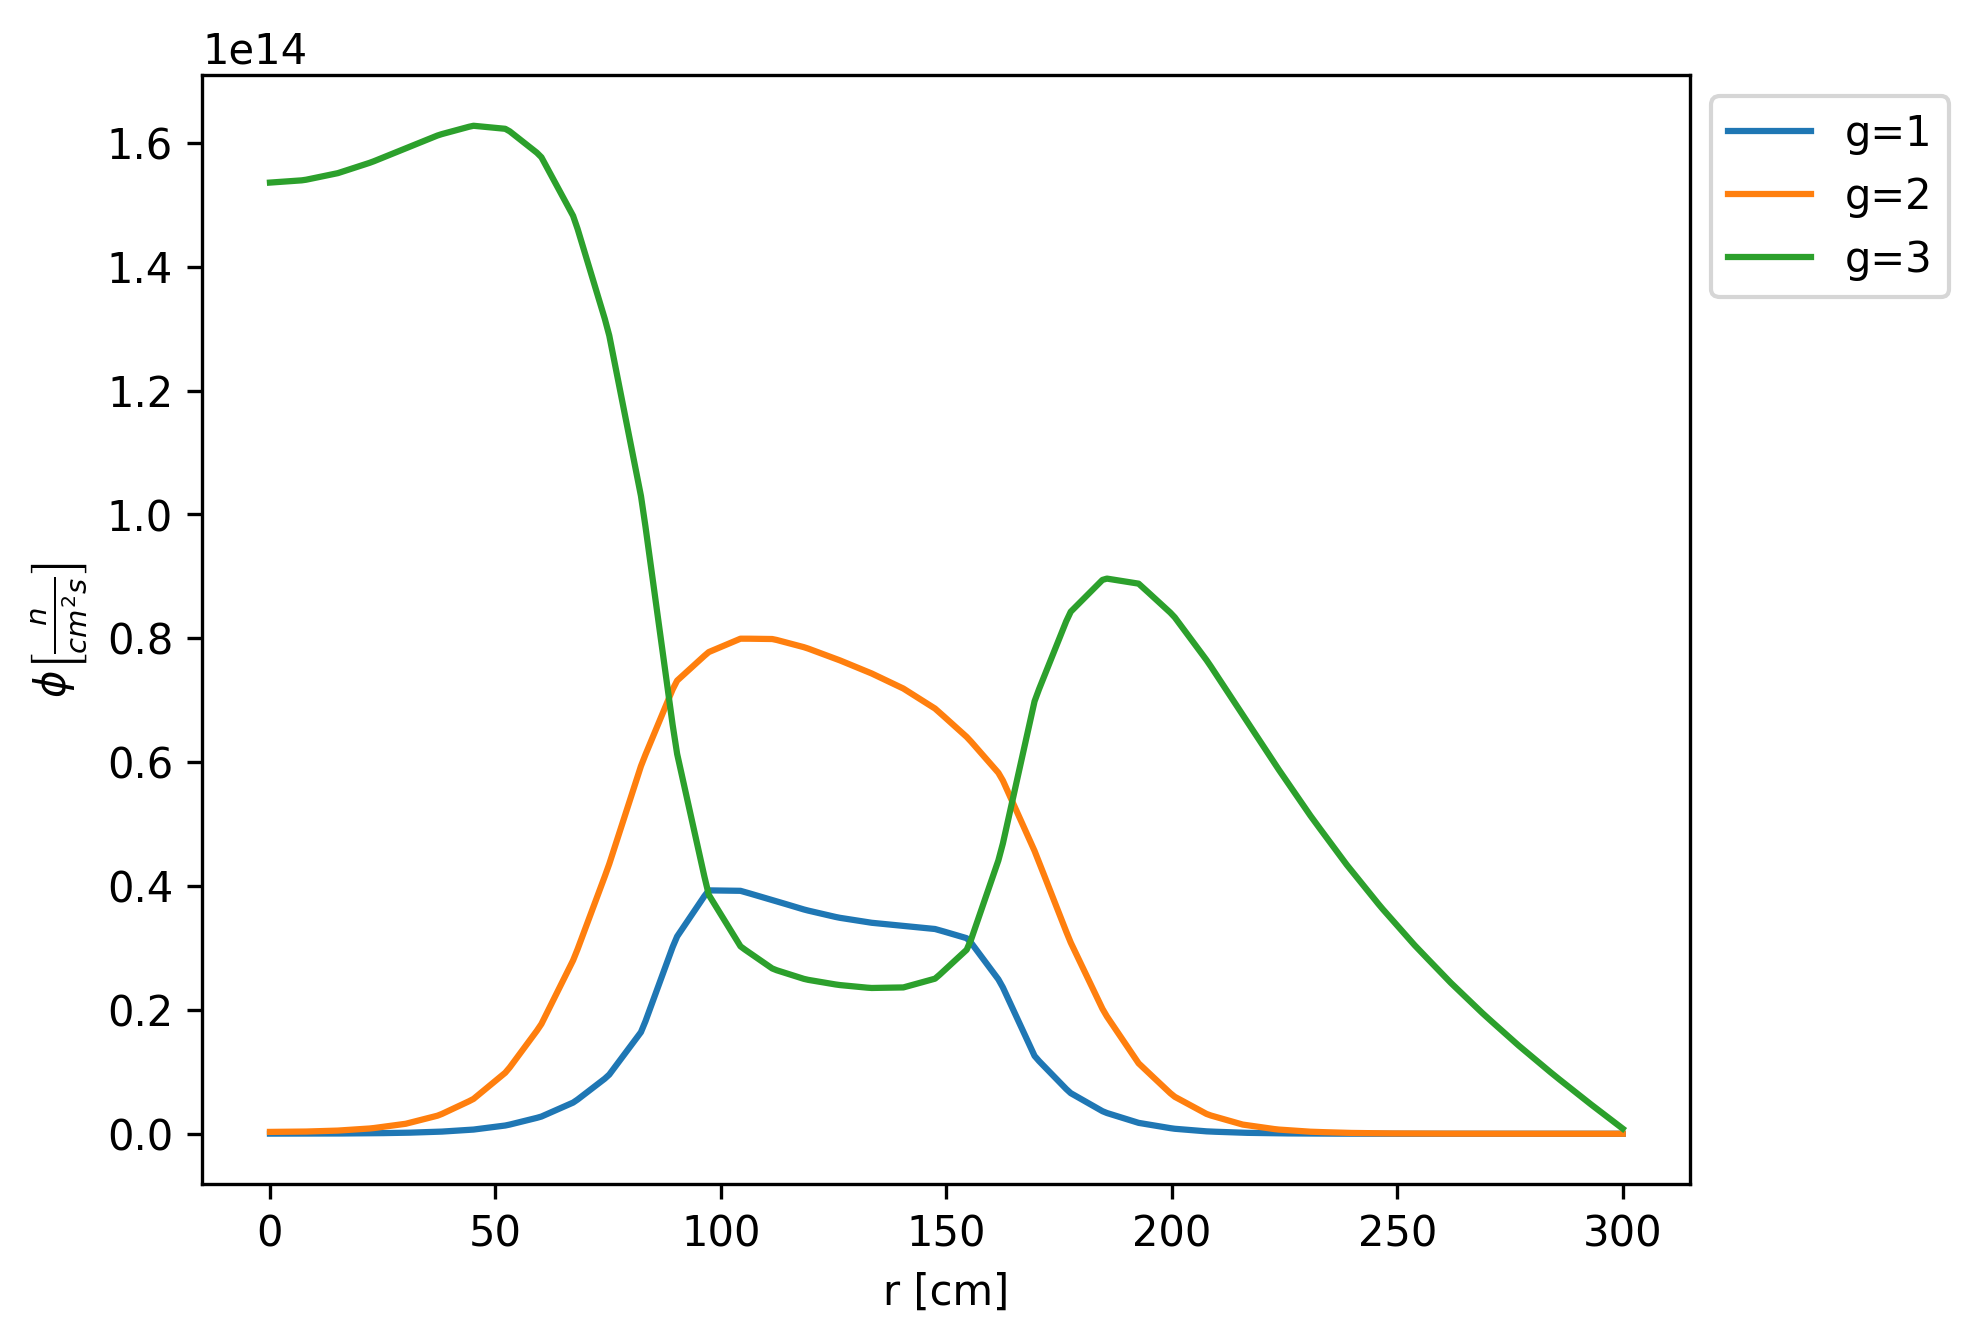
\includegraphics[width=0.45\textwidth]{figures-fullcore/3D-fullcore-1200-15Gc-radial1}
    }
    \subfloat[Serpent.]{
        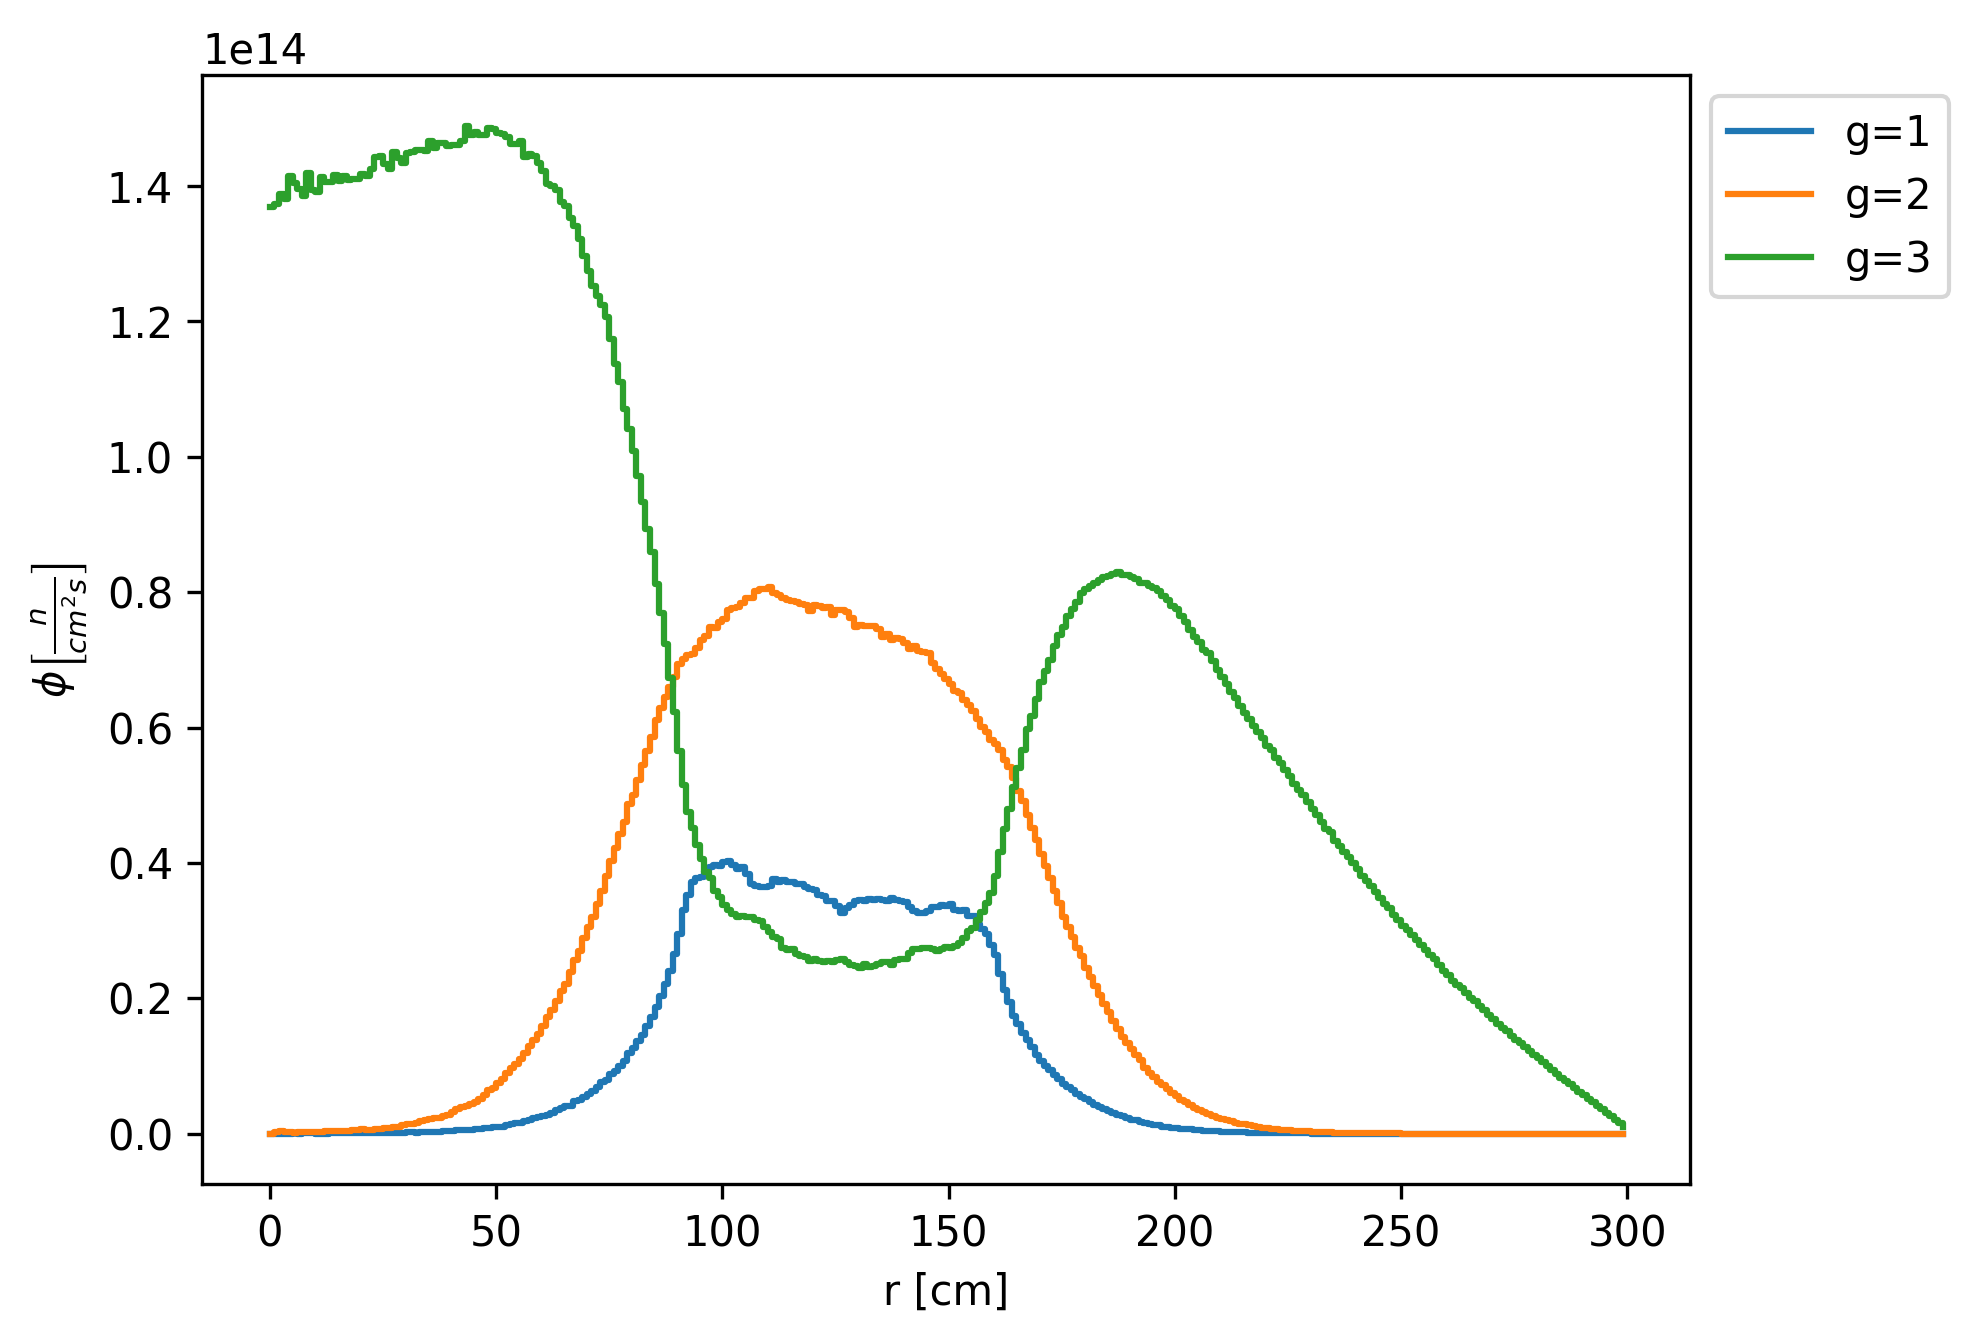
\includegraphics[width=0.45\textwidth]{figures-fullcore/serpent26G-1200-collapse-Radial}
    }
	\hfill
	\caption{Radial flux at 1200 K.}
	\label{fig:fullcore-1200-radial1}
\end{figure}


\section{OECD/NEA MHTGR-350 MW Benchmark: Phase I Exercise 1}

% Exercise description
This section conducted Phase I Exercise 1 of the benchmark with Moltres and compared the results with the already published results \cite{oecd_nea_coupled_2020}.
The benchmark specifies the cross-sections required to conduct the exercise.
This ensures a common dataset among various benchmark participants.
The files \textit{OECD-MHTGR350\_Simplified.xs} and \textit{xsmap.pdf} specify the group constants and the  constants numbering map.
The benchmark definition used DRAGON-4 \cite{marleau_user_2016} from a full block configuration.
The dataset contains 26 energy groups.
% What should be reported \cite{oecd_nea_benchmark_2017}
The exercise requests the reporting of the global parameters: $K_{eff}$, \gls{CR} worth ($\Delta \rho_{CR}$), and axial offset ($AO$).
% It also requires the reporting of a power distribution and a neutron-flux map \cite{oecd_nea_benchmark_2017}.
It also requires the reporting of a power distribution map \cite{oecd_nea_benchmark_2017}.
Equations \ref{eq:controlrod} and \ref{eq:ao} define $\Delta \rho_{CR}$ and $AO$.
\begin{align}
    \Delta \rho_{CR} &= \frac{k_{out}-k_{in}}{k_{out}k_{in}}
		\label{eq:controlrod}
    \intertext{where}
    k_{out} &= \mbox{eigenvalue with \gls{CR} at position 1184.8 cm} \\
    k_{in} &= \mbox{eigenvalue with \gls{CR} at position 391.81 cm}
		\intertext{and}
    AO &= (TP_{top}-TP_{bottom})/(TP_{top}+TP_{bottom})
		\label{eq:ao}
    \intertext{where}
    TP_{top} &= \mbox{total power produced in the top half core} \\
    TP_{bottom} &= \mbox{total power produced in the bottom half core.}
\end{align}

Figure \ref{fig:mesh} displays the geometry of the MHTGR-350.
The model included a one-third of the reactor.
The model considered the bottom and top reflectors.
The fuel consisted of 220 assemblies.
The simulations required two meshes. 
One for the control rod out (equation \ref{eq:controlrod}) and one for the control rod in.
The simulation with the control rod out had 268393 \glspl{DoF}/energy-group, and a total of 6978218 DoFs.
The simulation with the control rod in had 227592 \glspl{DoF}/energy-group, and a total of 5917392 DoFs.
The Moltres input files set an eigenvalue convergence tolerance of 1$\times$10$^{-8}$.

The benchmark exercise sets periodic boundary conditions on the the sides of the geometry.
However, a memory issue did not allow for the implementation of those boundary conditions in our 26-group Moltres input file.
We approximated the periodic boundary condition with the reflective boundary condition.
Section \ref{sec:bench-bcs} discusses further on the use of periodic and reflective boundary conditions.

% 4.33 h and 4.11 h
On average, the simulations took 4.22 hours using 1024 cores.
Table \ref{tab:globalparam} shows the main results.
Moltres predicted a \gls{Keff} larger than the reference result.
The reactivity difference is of 99 pcm.
Moltres yields a smaller control rod worth.
The difference is of 312 pcm.
The axial offset for the Moltres simulation is a 4$\%$ higher than the reference result.
We attribute the discrepancies to the use of the reflective boundary conditions instead of the periodic boundary conditions.
Once again, section \ref{sec:bench-bcs} discuss further on the use of periodic and reflective boundary conditions.

Figure \ref{fig:axialpower} shows the radially averaged axial power distribution.
Moltres results look close in shape and magnitude to the reference results.
Figure \ref{fig:radialpower} shows the axially averaged radial power distribution.
Moltres results are close to the reference results.
Moltres power distribution in the inner ring is larger.
The differences are within 0.25 W/cm$^3$.

\begin{figure}[htbp!]
	\centering
	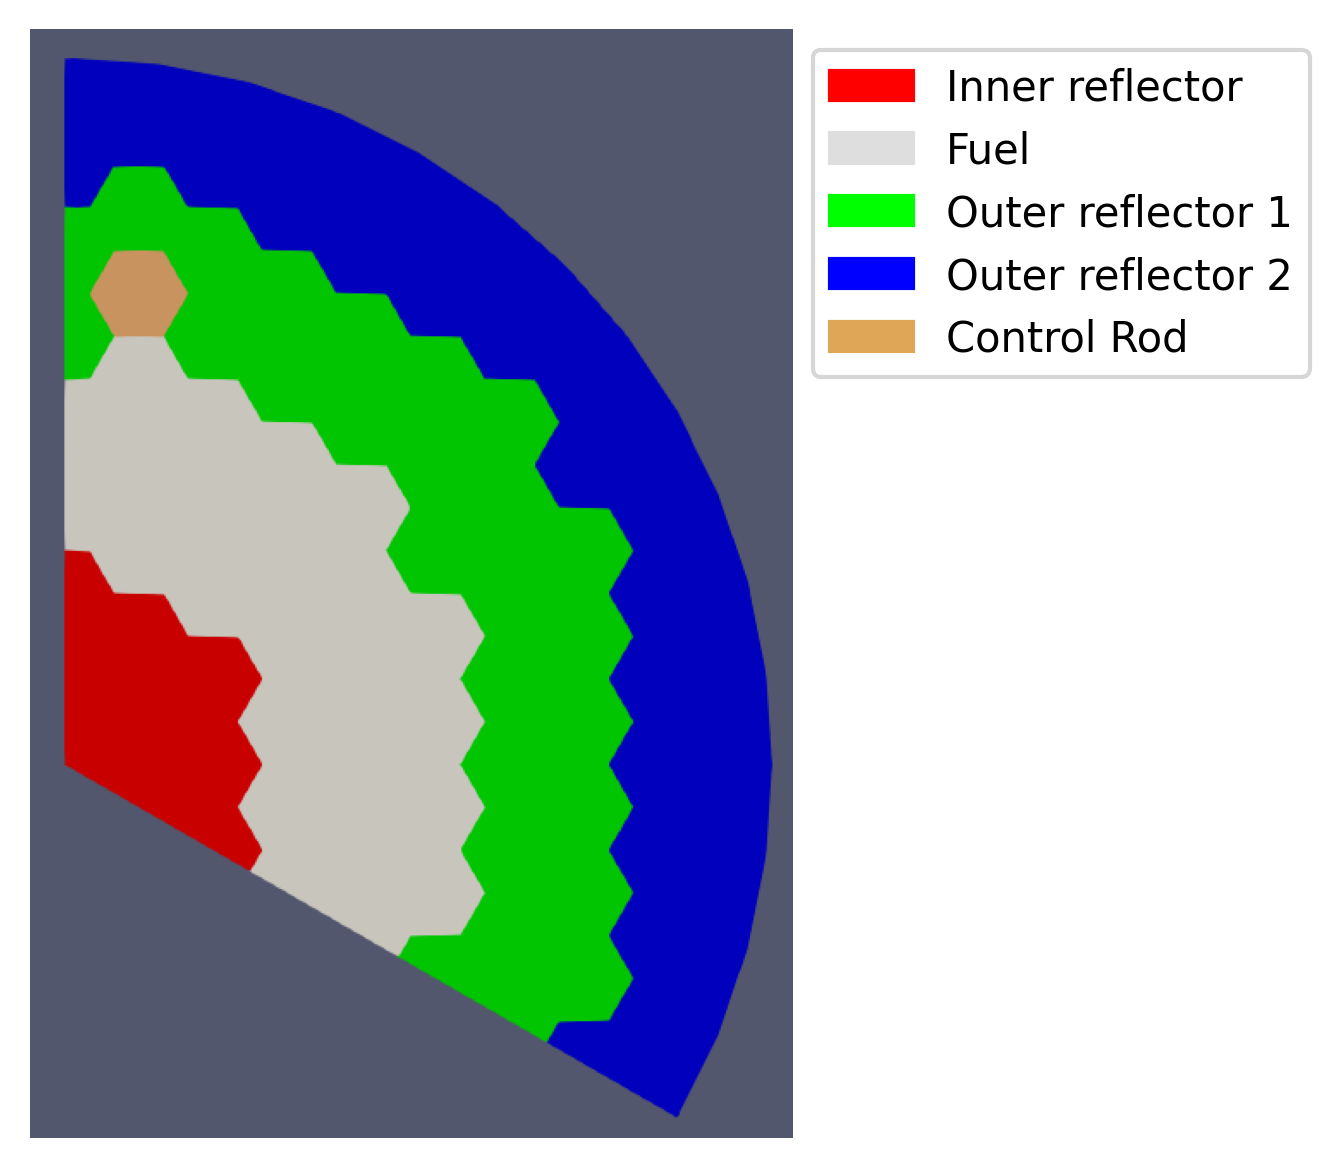
\includegraphics[width=0.55\linewidth]{figures-benchmark/oecd-fullcore-legend}
	\hfill
	\caption{1/3$^{rd}$ of the MHTGR-350 geometry.}
	\label{fig:mesh}
\end{figure}

\begin{table}[htbp!]
  \centering
  \caption{Global parameters.}
  \begin{tabular}{l|l|l}
  \toprule
  Parameter 	&  Benchmark  &  Moltres    \\
  \midrule
  K$_{eff}$ 	&  1.06691    &  1.06804    \\
  $\Delta \rho_{CR}$ [pcm]  & 822.1 	& 509.8 \\
  AO        	&  0.168      &  0.1753     \\
  \bottomrule
  \end{tabular}
  \label{tab:globalparam}
\end{table}

\begin{figure}[htbp!]
	\centering
    \subfloat[Moltres result.]{
        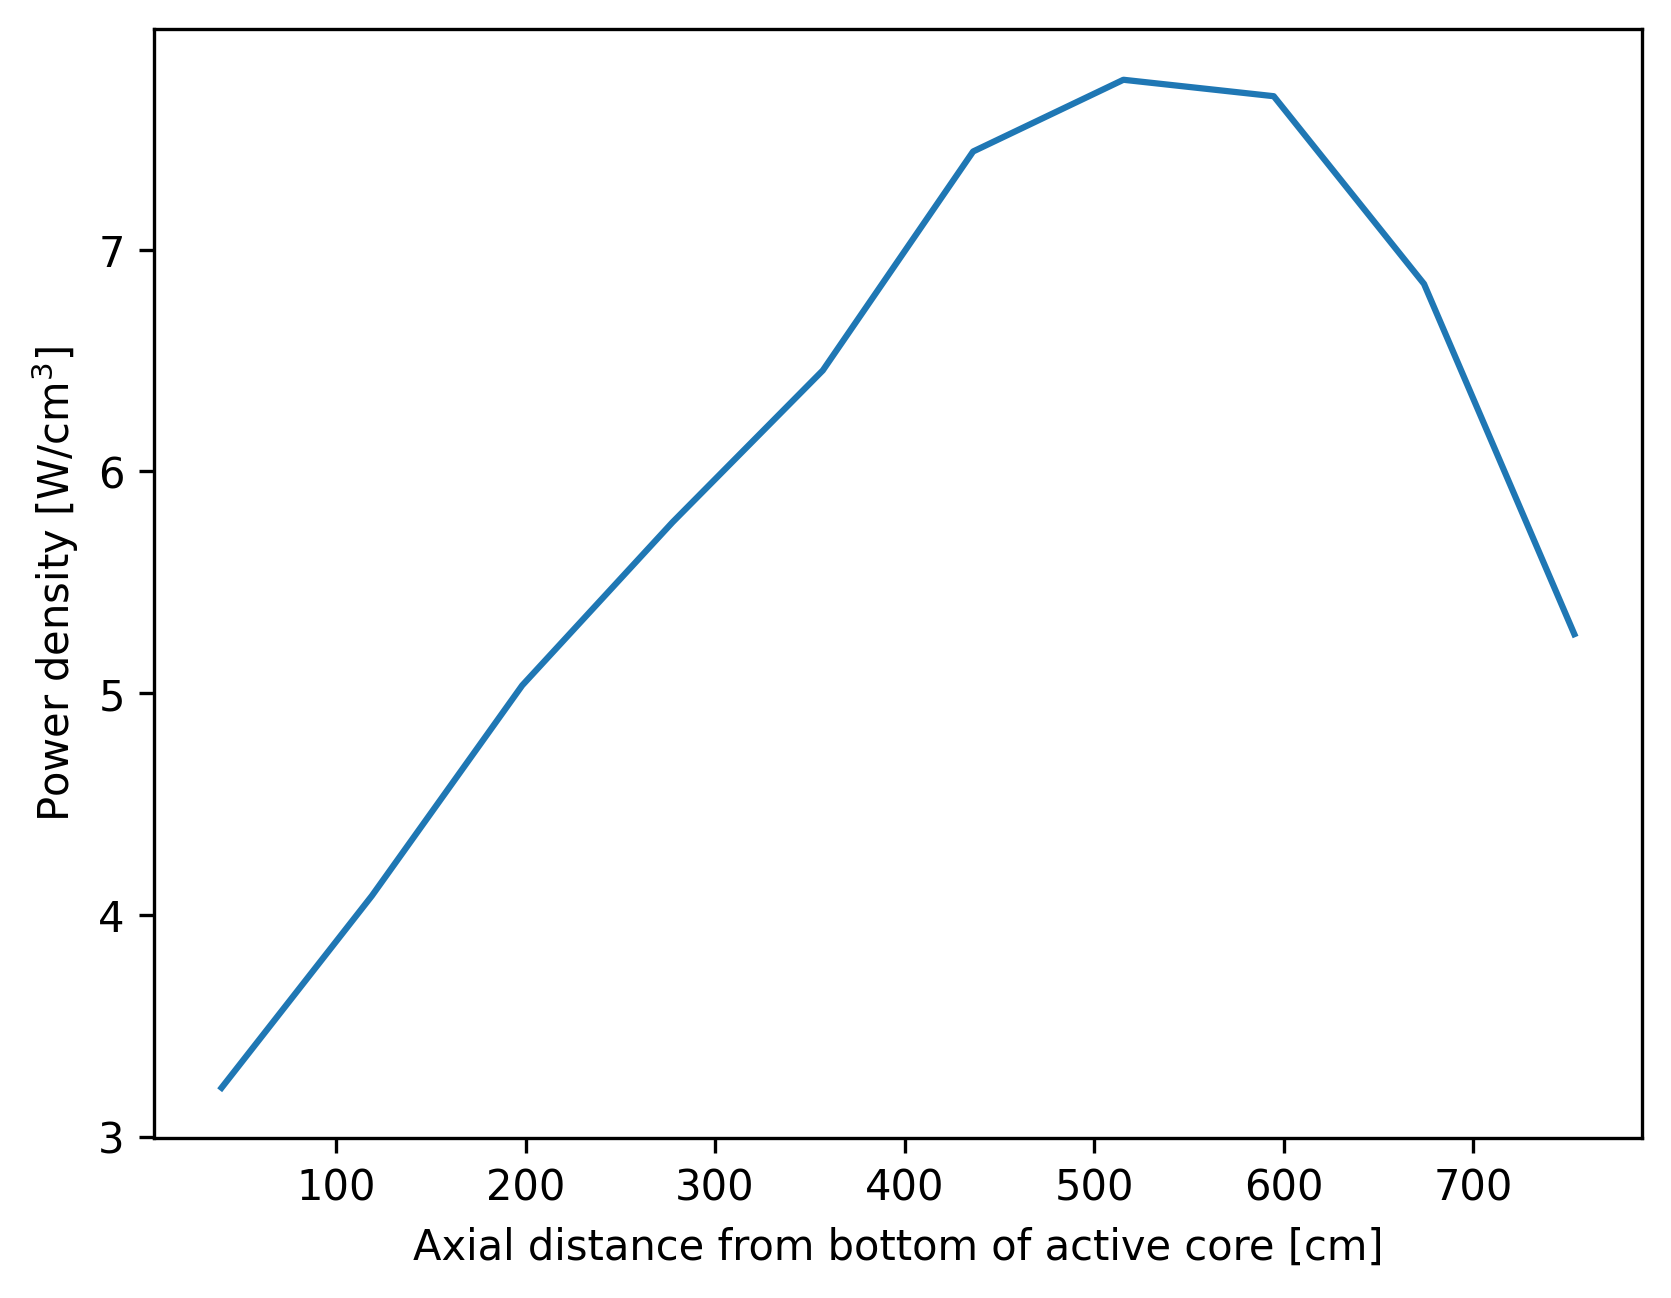
\includegraphics[width=0.42\textwidth]{figures-benchmark/3D-fullcore26G-axialpower}
    }
    \subfloat[Benchmark result. Image reproduced from \cite{oecd_nea_coupled_2020}.]{
        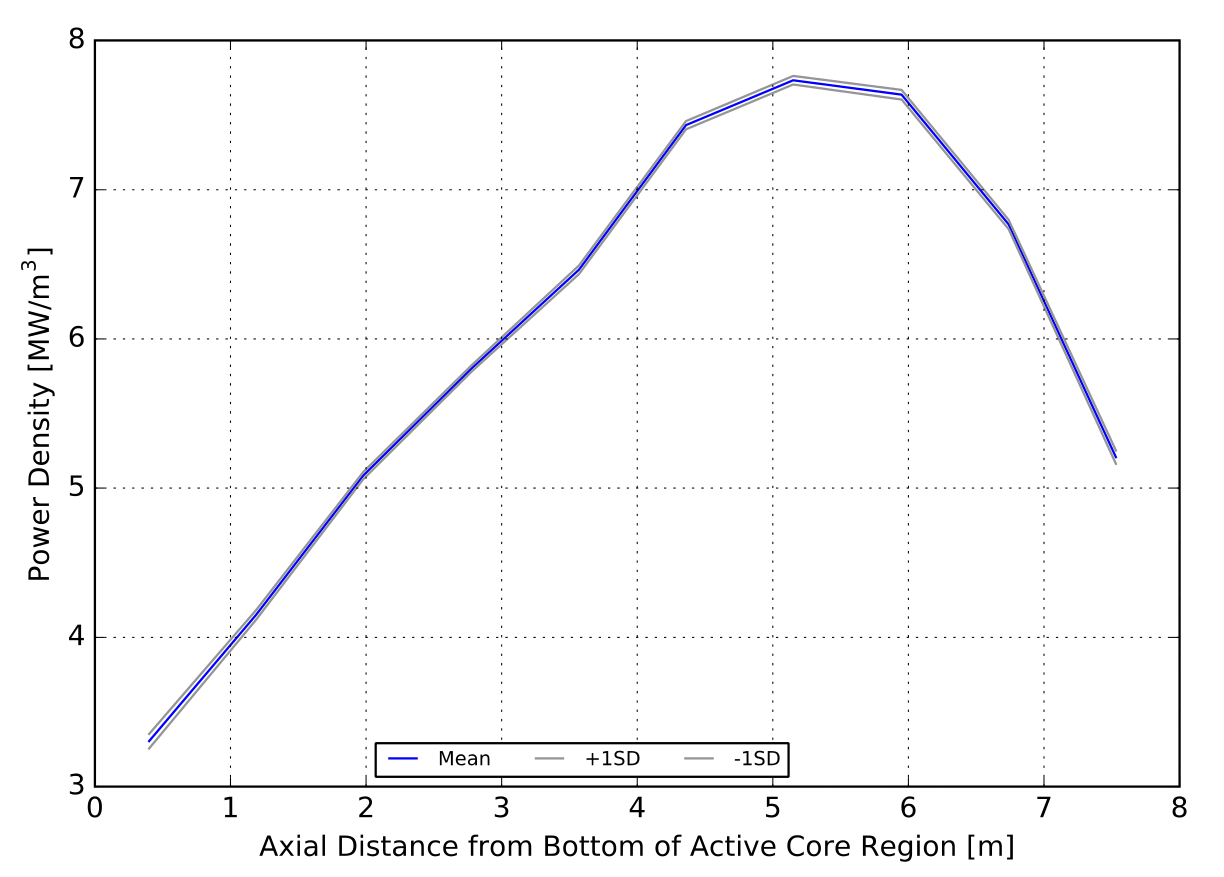
\includegraphics[width=0.47\textwidth]{figures-benchmark/benchmark-axialpower}
    }
	\hfill
	\caption{Radially averaged axial power distribution.}
	\label{fig:axialpower}
\end{figure}

\begin{figure}[htbp!]
	\centering
    \subfloat[Moltres result.]{
        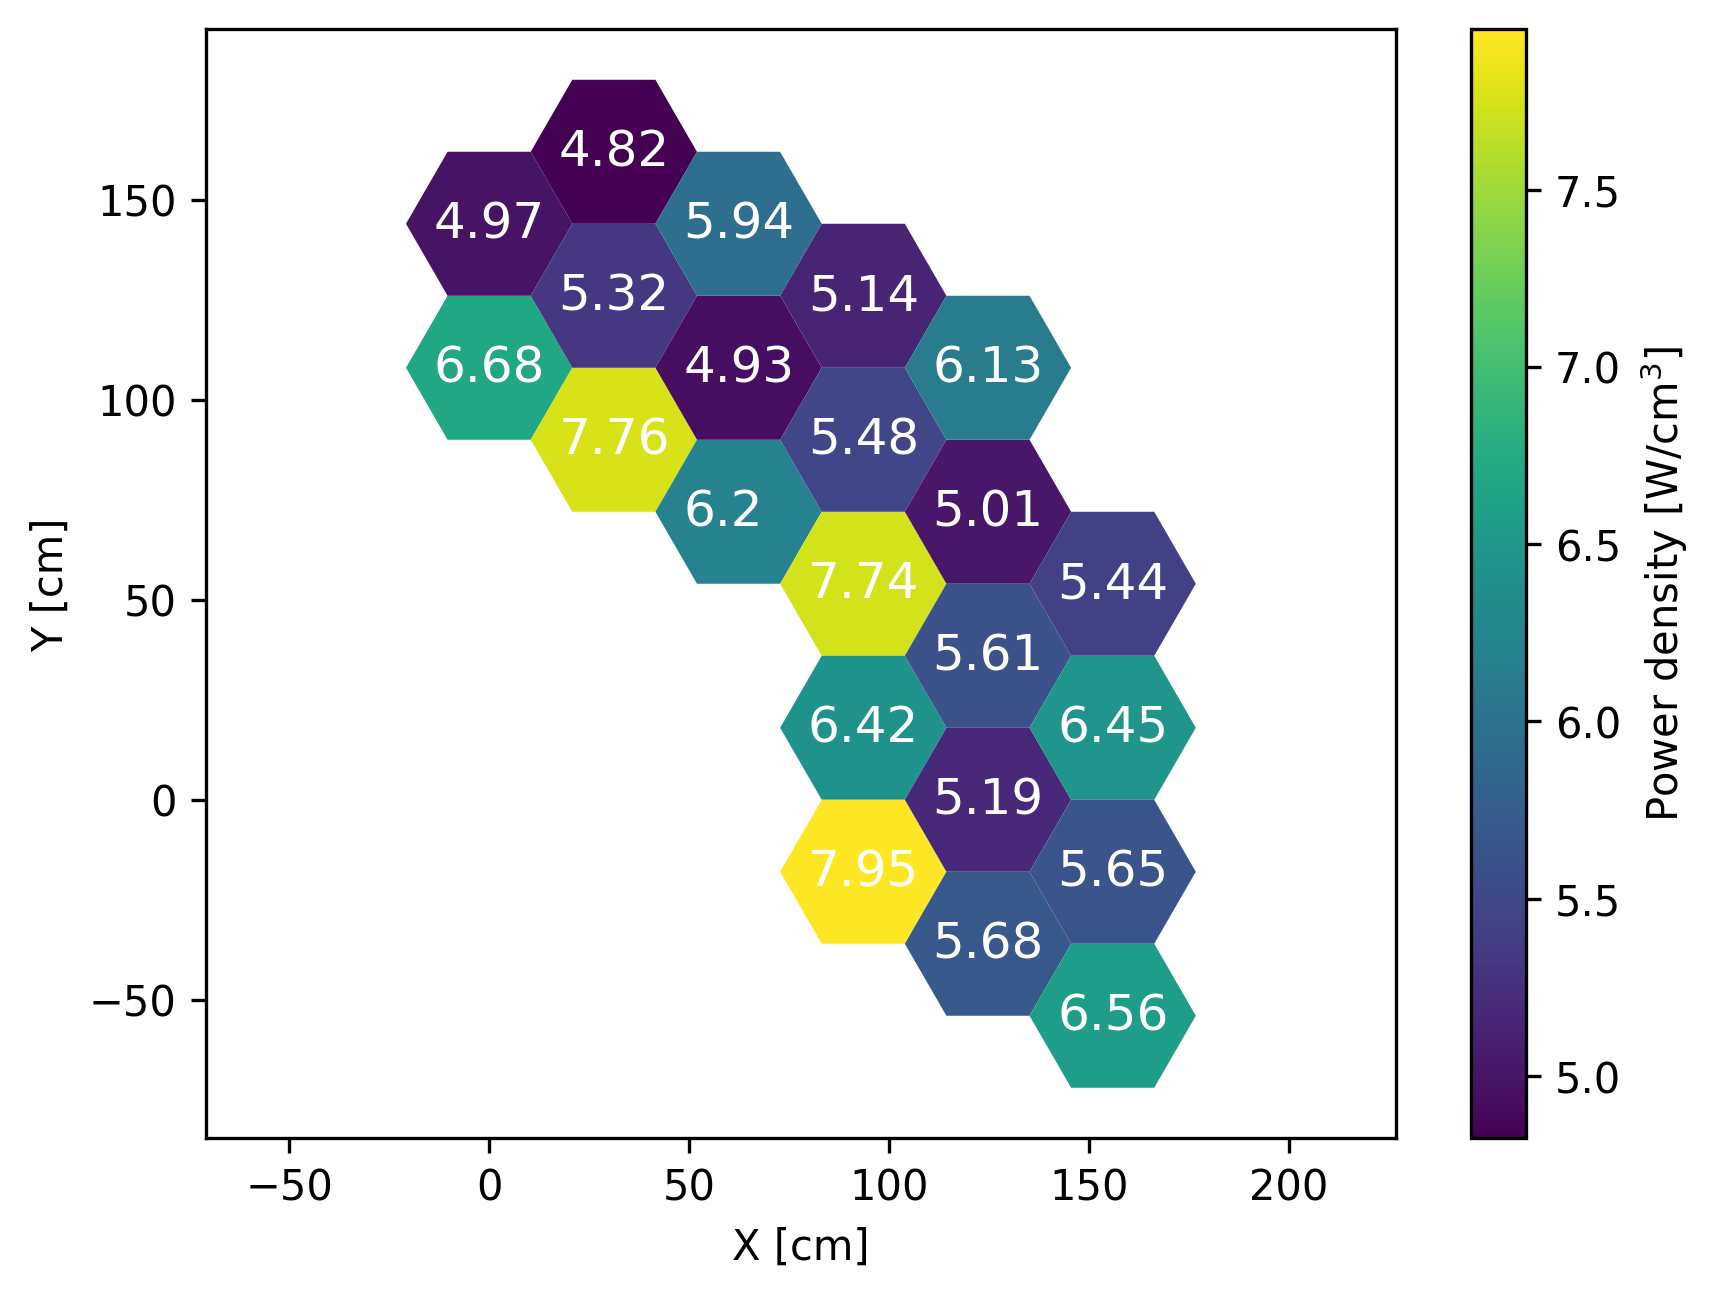
\includegraphics[width=0.41\textwidth]{figures-benchmark/3D-fullcore26G-radialpower}
    }
    \subfloat[Benchmark result. Image reproduced from \cite{oecd_nea_coupled_2020}.]{
        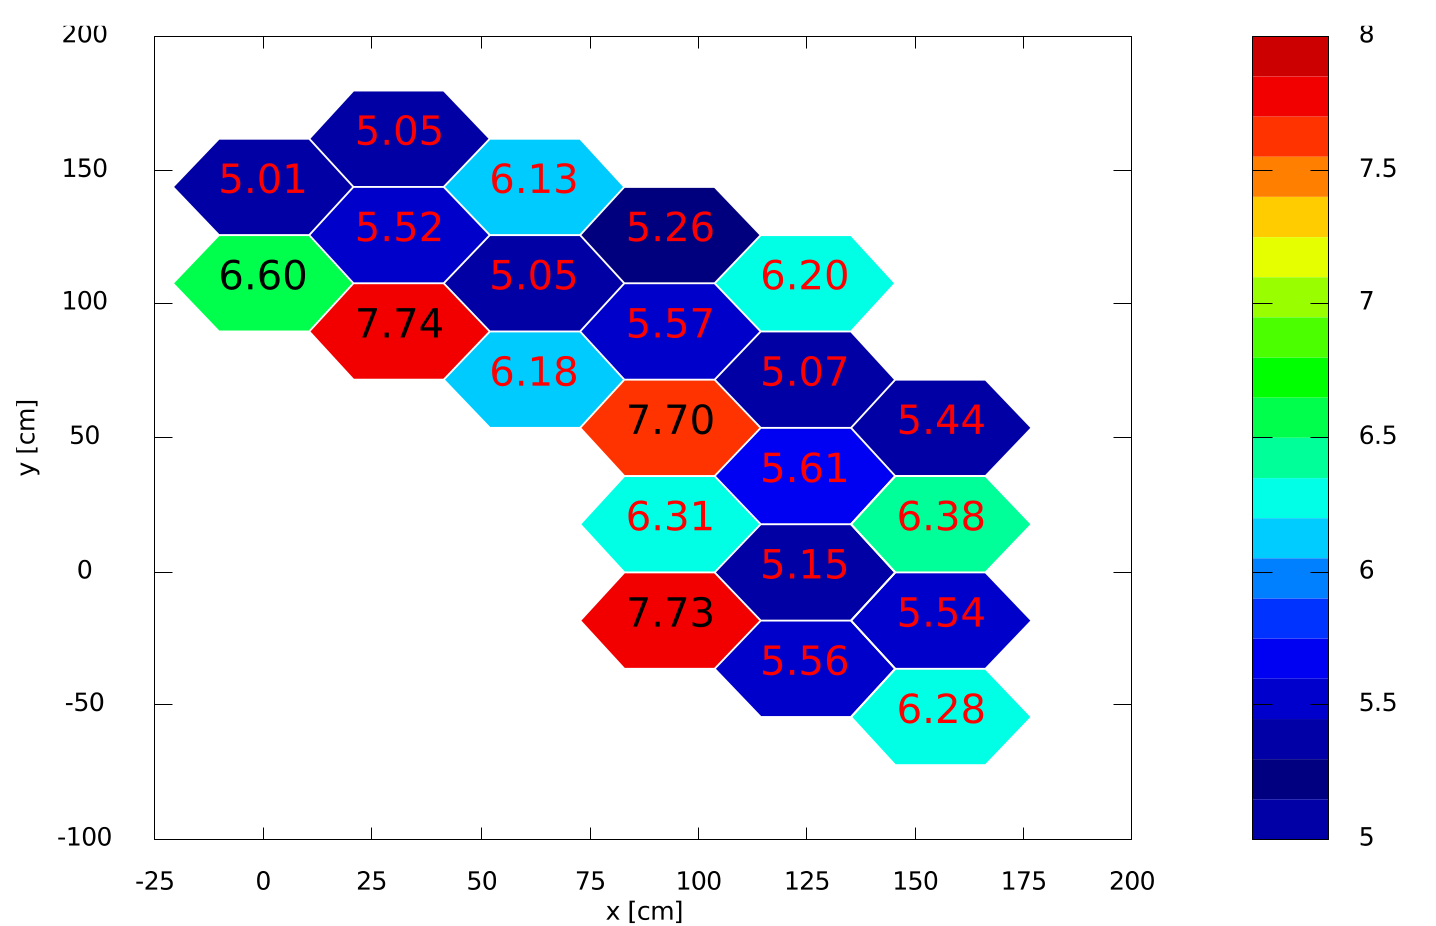
\includegraphics[width=0.49\textwidth]{figures-benchmark/benchmark-radialpower}
    }
	\hfill
  \caption{Axially averaged radial power distribution.}
  \label{fig:radialpower}
\end{figure}

\subsection{Periodic vs Neumann BCs}
\label{sec:bench-bcs}

In the last section, we observed deviations in Moltres results.
In this section, we analyzed the discrepancies that the reflective boundary condition approximation may introduce.
As the last section mentioned, the memory requirements of the simulation limit the use of the periodic boundary conditions.
To reduce the memory requirements, we collapsed the group constants to a smaller number of energy groups.
We simulated two cases: one that uses a 3-group structure and one that uses a 6-group structure.
The simulations required two meshes each.

The 3-group simulation had 62118 DoFs/energy-group (total of 186354 DoFs) and 61596 DoFs/energy-group (total of 184788 DoFs) for the control rod out and control rod in cases, respectively.
The 6-group simulation had 16898 DoFs/energy-group (total of 101388 DoFs) and 19116 DoFs/energy-group (total of 114696 DoFs) for the control rod out and control rod in cases, respectively.
We highlight that the 6-group simulation had to use a coarser mesh, otherwise it would not run.
This confirms the suspicion that the simulation's memory requirements prevents it from running.

For both cases, we ran simulations with periodic and neumann boundary conditions and we compared their results.
Table \ref{tab:benchmark-bc} presents the results.
The neumann boundary condition increases the $K_{eff}$.
For the control rod out case, the increase is small.
However, for the control rod in case, the increase is considerable.
The combined effect of both increases leads to a decrease in the control rod worth.
The axial offset results almost unaffected by the boundary condition approximation.

\begin{table}[htbp!]
  \centering
  \caption{Global parameters comparison for different types of BCs.}
  \begin{tabular}{l|l|l|l|l|l}
  \toprule
  Energy groups       & Type of BCs & K$_{eff, out}$ & K$_{eff, in}$ & $\Delta \rho_{CR}$ [pcm] & AO \\
  \midrule
  \multirow{2}{*}{3}  & Periodic    & 1.07571		& 1.06776		& 692.6		& 0.237		\\
                      & Neumann     & 1.07586	  & 1.07021   & 490.5		& 0.237	  \\ \hline
  \multirow{2}{*}{6}  & Periodic    & 1.07182		& 1.06356		& 724.3	  & 0.185  	\\
                      & Neumann     & 1.07197   & 1.06610 	& 513.3		& 0.186		\\  
  \bottomrule
  \end{tabular}
  \label{tab:benchmark-bc}
\end{table}

\section{Conclusions}

% Preliminary studies: homogeneous vs heterogeneous isotopic distribution
The preliminary studies focused on several aspects of the simulations.
The first aspect was the effect of distributing homogeneously the fuel compact isotopes in the Serpent model.
The heterogeneous calculation took 28$\%$ more time.
The results showed that the multiplication factor decreases considerably.
Additionally, the homogenization of the fuel compact appears not to have a strong impact over the group constants.
However, the considerable difference in the multiplication factor suggests that the combined effect of small variations in the group constants is significant.
Although the particles’ explicit modeling is time-consuming, it results necessary.

% Preliminary studies: homogeneous vs heterogeneous diffusion simulation

% Serpent-Moltres: Fuel column
Focusing on a fuel column of the MHTGR-350, we investigated the effects of the energy group structure on the diffusion calculations.
We considered four different operational cases: a fuel column without LBPs and a fuel column with LBPs, both cases at 600K and 1200K.
Serpent obtained the homogenized group constants of the fuel column.
Moltres took such constants as input with a Gmsh mesh.
The first study compared the Moltres axial flux to Serpent axial flux.
Moltres used a 26 energy group structure to run the simulations.
Overall, the axial fluxes were close in shape and magnitude.
A different study focused on the effects of the energy group structure on the \gls{Keff}.
We note that the number of energy groups does not affect the accuracy of the eigenvalue calculations in Moltres.
We also compared the $L_2$-norm relative error of the axial flux in the active core using different energy group structures.
For the four operational cases, the accuracy improves increasing the number of energy groups.
Additionally, we presented the simulation computational expense for the different number of energy groups.
The simulation time and memory requirement rises increasing the number of energy groups.
We notice as well that the computational time increases for the fuel column with LBPs.
Finally, we analyzed the impact of using different 15-group structures on the $L_2$-norm relative error of the axial flux.
We chose the $15d$ structure as the best performing.

% Serpent-Moltres: Full-core
Based on the results from the fuel column analysis, we compared Moltres full-core results to Serpent reference results.
We considered two operational cases: 600K and 1200K.
Serpent obtained the homogenized group constants of the different regions of the reactor.
Moltres took such constants as input with a Gmsh mesh.
The first analysis compared the Serpent and Moltres eigenvalues.
Moltres results were bigger.
The overall difference was less than 300 pcm.
The second analysis compared the radial power distributions from both codes.
These results showcase the symmetry of the problem.
To reduce the computational expense other simulations could reduce the problem size by a half.
Overall, Moltres radial power distribution shows close proximity to the Serpent's result.
We also compared the flux shape and magnitude.
The axial fluxes show small discrepancies, mostly in their magnitude.
The radial fluxes are close in shape and magnitude.
However, the radial flux in the diffusion calculation fails to capture the steep flux close to the LBPs.
Overall, the fluxes are similar.

% OECD-Benchmark
The simulation capabilities for HTGRs has not reached the state of the art of LWRs.
This delay in the development of such capabilities has motivated OECD/NEA to define a benchmark to carry out code-to-code comparisons.
The benchmark uses the MHTGR-350 as the reference design.
We conducted Phase I Exercise 1 with Moltres.
The benchmark defines the group constants for the exercise.
The group constants have a 26-energy group structure.
The benchmark exercise sets periodic boundary conditions on the the sides of the geometry.
Such implementation in Moltres has been challenged by the simulation high memory requirements.
To go around such barrier, we approximated the periodic boundary condition with a reflective boundary condition.
Two out of three global parameters exhibit good agreement with the reference results.
However, the control rod worth presents a large discrepancy.
Such a discrepancy rises from the approximation in the boundary conditions.
The use of a reflective boundary condition for the control rod out case does not have a strong impact over the \gls{Keff}.
On the other hand, the choice of boundary condition for the control rod in case has a substantial effect.
The combined effect of the approximation leads to large error in the control rod worth.
The approximation has a small influence on the axial offset.

\pagebreak
\bibliographystyle{plain}
\bibliography{bibliography}

\end{document}
